\documentclass	[11pt, a4paper, openany]{book}
\usepackage[utf8]{inputenc}
\usepackage[francais]{babel}
\usepackage[T1]{fontenc}
\usepackage{amsmath}
\usepackage{amsfonts}
\usepackage{amssymb}
\usepackage{lmodern}
\usepackage{amsthm}

\usepackage{graphicx} % ajout image
\usepackage[tt]{titlepic}%Centre le titre

\usepackage{shorttoc} %Permet d'avoir de petites tables des matières


\usepackage{shapepar} %texte en keur
\usepackage{siunitx} %S.I.

\usepackage{graphicx}
\usepackage{caption} %Permet d'ajouter des légendes en images sans les mettre en float + ds la marge
\usepackage{delarray} % Belles matrices

\usepackage{fancyhdr} %Permet de modifier l'entête & footer
\usepackage{bbding} % Note marge
\usepackage{todonotes}
\usepackage{wrapfig}

\pagestyle{headings} % Titre du ch et numéro page dans l'entete
\usepackage{fullpage} %Utilise toute la page


\usepackage{verbatim} %Commentaire multi-lignes

\newcommand{\cst}{\text{cst}}
\newcommand{\E}{\vec E}
\newcommand{\F}{\vec F}

\newcommand{\questpm}[3]{#1. \textbf{#3} (p.#2)}
\newcommand{\exerc}[2]{\textbf{\Large Exercice #1\normalsize \\#2}}
\newcommand{\dif}{\mathrm{d}}
%\newcommand{\comment}[1]{}
\newcommand{\rot}{\text{rot}\,}
\newcommand{\divv}{\text{div}\,}
\newcommand{\phas}[1]{\underline{#1}}
\newcommand{\RE}{\text{Re}}
\DeclareMathOperator{\arccot}{arccot}
\newcommand{\com}[1]{}

%\newcommand{\oiint}{\int\!\!\!\!\!\:\!\!\!\;\!\!\subset\!\!\supset\!\!\!\:\!\!\!\!\!\int}
\newcommand{\oiint}{\int\!\!\!\!\!\!\! \:\!\subset\!\!\supset\!\!\!\!\!\!\!\int}



\begin{document}
\renewcommand{\proofname}{Démonstration}
\frontmatter
\begin{titlepage}
\begin{center}	
	
	\newcommand{\HRule}{\rule{\linewidth}{0.5mm}}   			%Titre en gros
	
\includegraphics[scale=0.11]{logo.jpg}~\\[1cm]				%Logo

	\textsc{\LARGE Université Libre de Bruxelles}\\[1.5cm]
	\textsc{\Large Synthèse}\\[0.5cm]

	\HRule \\[0.4cm]
	{ \huge \bfseries Physique générale \\[0.4cm] }


	\HRule \\[1.5cm]
		\begin{minipage}{0.4\textwidth}
		\begin{flushleft} \large
		
		\emph{Auteur:}\\
			Nicolas \textsc{Englebert}\\
			\end{flushleft}
			\end{minipage}
			\begin{minipage}{0.4\textwidth}
			\begin{flushright} \large
			\emph{} \\		
			\textsc{}
			\end{flushright}
		\end{minipage}

	\vfill

% Bottom of the page
{\large \today}

\end{center}
\end{titlepage}





\part{Introduction}
\chapter{A propos du document}
Les notes en flèche = information supplémentaires sur un point précis (flèche pour cibler le mot)
Les cadre sans flèche = Information générale
Sans cadre = réflexion générale (pas encore utilisé)
Les cadres dans texte = formule finale
Notes en bas de page = petite info




\mainmatter
\part{Synthèse du cours}
\chapter{Thermodynamique}
\section{Introduction}
Une brève introduction aux degrés de libertés. Une lecture attentive suffira.

\section{La pression}

\begin{wrapfigure}[10]{l}{4cm}
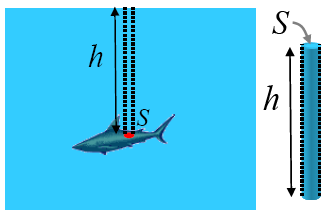
\includegraphics[width=4cm]{th/image1.png}
\captionof{figure}{Pression hydrostatique}
\end{wrapfigure}

Dans notre cas, le poids est la force engendrée par la colonne d'eau. Comme celle-ci est liquide, sont poids vaut $\underbrace{\rho V}_m  g$.\\
Par définition, de la pression : $P \equiv \frac{Poids}{Surface}$ on peut trouver la pression hydrostatique \footnote{Que pour des liquides incompressibles} :
\begin{equation}
P_{hydrostatique} = \rho g h
\end{equation}
Les unités de la pression sont les Pascals $\left(Pa = \dfrac{N}{m^2}\right)$. Notons également que 1 bar = $10^5\ Pa$ et que $1\ atm = 1,013\ bar$.

\subsection{Le baromètre}
\begin{wrapfigure}[10]{r}{3cm}
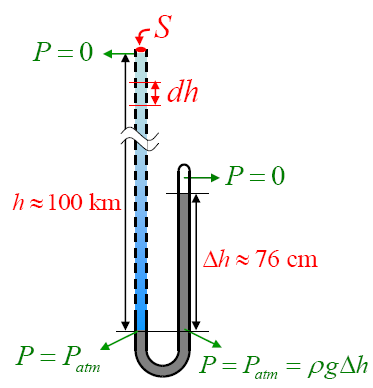
\includegraphics[scale=0.3]{th/image2.png}
\captionof{figure}{Baromètre}
\end{wrapfigure}
Son but est de mesurer la pression atmosphérique. La colonne d'air au dessus de nous à une hauteur de 100km. Si l'air était du mercure, cette colonne ferait 76mm de hauteur. \\

Ici l'air n'est pas un liquide incompressible, il faut donc passer par le formalisme intégral : 
\begin{equation}
Poids\ =\ \rho_{air}.g.s.dh
\end{equation}
Connaissant la définition de la pression, on peut calculer celle-ci
\begin{equation}
\int_0^h \frac{\rho_{air}g.S.dh}{S} = \rho_air.g.\Delta h
\end{equation}

\section{La température}
\subsection{Dilatation thermique}
Utilisation de la dilatation dans les thermomètres (Même si aujourd'hui on utilise de l'alcool, initialement c'était avec un gaz).

\subsection{Température absolue}
A l'aide d'un thermomètre à gaz à volume constant, \textit{Amontons} a mis en évidence une relation linéaire entre la pression et la température.
\begin{center}
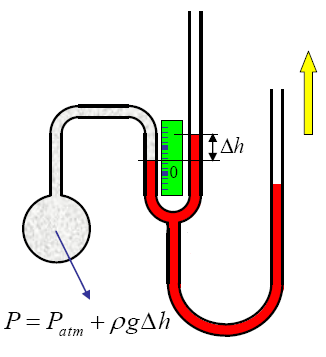
\includegraphics[scale=0.15]{th/image3.png}
\captionof{figure}{Thermomètre à gaz à volume constant}
\end{center}
\begin{equation}
P = \alpha T + P_0
\end{equation}
où $P_0$ est la température à $0 deg. C$.\\
En extrapolant les résultats par une série de mesure répétitive, \textit{Amontons} a pu mettre en évidence l'existence du zéro absolu (-273,15 deg. C)
\begin{center}
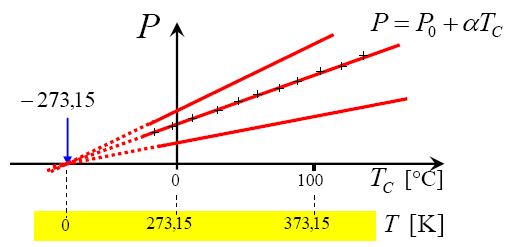
\includegraphics[scale=0.3]{th/image4.png}
\captionof{figure}{Extrapolation du zéro absolu}
\end{center}

\section{Comportement des gaz}
\subsection{Loi de Gay-Lussac (Amontons)}
Cette loi est la même que celle découverte par \textit{Amontons}. Elle dit que la pression est proportionnelle à la température à volume constant.
\begin{equation}
P \propto T|_{V = cste}
\end{equation}

\subsection{Loi de Charles}
\begin{wrapfigure}[7]{l}{3cm}
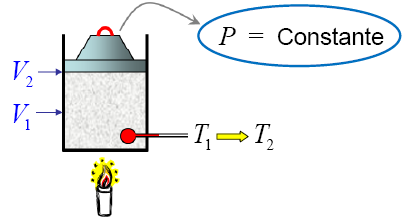
\includegraphics[scale=0.23]{th/image5.png}
\captionof{figure}{Loi de Charles}
\end{wrapfigure}
Par le placement d'un poids libre de se mouvoir, la pression est maintenue constante. Ceci permis l'étude de l'élévation du piston à pression constante et de dériver la Loi de Charles :
\begin{equation}
V \propto T|_{P = cste}
\end{equation}

\subsection{Loi de Boyle et Mariotte}
Ces deux scientifiques ont mis en évidence une relation entre le volume et la pression à température constante :
\begin{equation}
PV = cste|_{T = cste}
\end{equation}

\subsection{Loi des gaz parfaites}
En rassemblant les trois lois obtenues ci-dessus, on obtient : 
\begin{equation}
PV = \alpha T
\end{equation}
Si l'on devait doubler le nombre de particules de gaz, la constante $\alpha$ serait proportionnelle au nombre de particules multiplié par une constante ($\alpha \propto N.cste$).\\
Pour des raisons détaillée ci-dessous, $\alpha = N.k_B$ de la sorte que
\begin{equation}
PV = N.k_BT
\end{equation}

\subsection{Loi d'Avogadro}
Le but est de déterminer la valeur de la \textit{constante de Boltzman}, $k_B$ grâce à la loi d'Avogadro : Si la pression et la température sont constantes, la volume $V$ occupé par $N$ particules est le même.\\ Ce n'est donc pas le nombre d'atomes qui détermine le volume. En isolant $V$ :
\begin{equation}
V = k_B . \frac{NT}{P}
\end{equation}
Or, $\frac{NT}{P}$ donnant une valeur unique pour un gaz, $k_B$ est une constante universelle. \\En posant $P=1atm, T = 237,15K, V = 22,4 L$ on trouve :
\begin{equation}
k_B = 1,38.10^{-23}\ \frac{Pa.m^3}{K}\ \ \  \left(= \frac{N.m^3}{m^2.K} = \frac{J}{K}\right)
\end{equation}

\subsection{Constante universelle des gaz parfaits}
Le nombre de moles étant donné par $n = N/N_A$, on déduit que $N = n.N_A$. En substituant dans la loi des gaz parfaits\footnote{Valabie si $P$ pas trop grande et $T$ pas trop petite} :
\begin{eqnarray}
PV &=& n.\underbrace{N_A.k_B}_R T\\
PV &=& nRT
\end{eqnarray}
où $R\ =\ 8,314\ J/K$.

\section{Théorie cinétique des gaz parfaits}
Un gaz est un ensemble de particules en mouvement incessant (dit parfait s'il $\nexists$ d'interactions entres particules). Chaque particule cause un impact générant une pression.
\begin{equation}
Force\ d'impact\ : f = m\frac{dv}{dt}
\end{equation}

\subsection{Incidence normale}
Lors d'un impact, la particule s'écrase et regagne une accélération.
\begin{center}
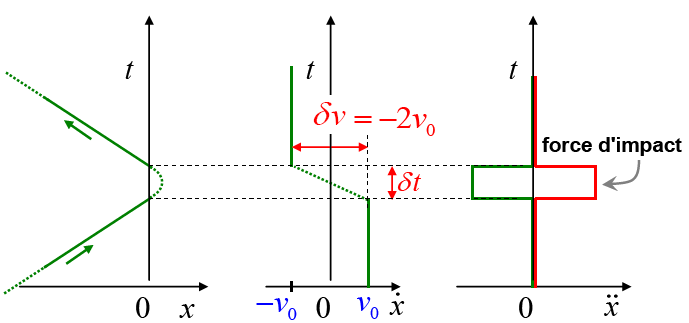
\includegraphics[scale=0.4]{th/image6.png}
\captionof{figure}{Incidence normale : Position - Vitesse - Accélération}
\end{center}
En prenant l'hypothèse que l'accélération est constante $\ddot{x} = a = cste$ on peut trouver la vitesse par intégration  : $\dot{x} = at + C$.\\
Grâce à $f = ma$, on peut calculer la force d'impact (on suppose $dv/dt = \partial v / \partial t$ (hypoth. de modél.comme $V = cste$)) sachant que la vitesse vaut = $v = -v_0 - v_0 = -2v_0$ (voir schéma ci-dessus)
\begin{equation}
f = m\ddot{x} = m\frac{dv}{dt} = m\frac{\partial v}{\partial t} = -m\frac{2v_0}{\partial t}
\end{equation}
Comme $\overline{f_i} = -f$, la force d'impact moyenne vaut :
\begin{equation}
\overline{f_i} = m \frac{2v_0}{\partial t}\vec{1_x}
\end{equation}
Le signe est positif car la force se dirige vers les $x > 0$  (Action/réaction)

\subsection{Incidence oblique}

















\chapter{Électrostatique}

Lorem ipsum dolor sit amet, consectetur adipiscing elit. Sed non risus. Suspendisse lectus tortor, dignissim sit amet, adipiscing nec, ultricies sed, dolor. Cras elementum ultrices diam. Maecenas ligula massa, varius a, semper congue, euismod non, mi. Proin porttitor, orci nec nonummy molestie, enim est eleifend mi, non fermentum diam nisl sit amet erat. Duis semper. Duis arcu massa, scelerisque vitae, consequat in, pretium a, enim. Pellentesque congue. Ut in risus volutpat libero pharetra tempor. Cras vestibulum bibendum augue. Praesent egestas leo in pede. Praesent blandit odio eu enim. Pellentesque sed dui ut augue blandit sodales. Vestibulum ante ipsum primis in faucibus orci luctus et ultrices posuere cubilia Curae; Aliquam nibh. Mauris ac mauris sed pede pellentesque fermentum. Maecenas adipiscing ante non diam sodales hendrerit.























\chapter{Magnétostatique}
\section{Introduction}
Rien de bien important, une bonne lecture et ça ira!

\section{Courants électriques et champ magnétique}
Oersted a mis en avant que le courant électrique génère un champ magnétique perpendiculaire au sens du courant, grâce à l'expérience de la boussole.\\

\begin{wrapfigure}[7]{l}{4cm}
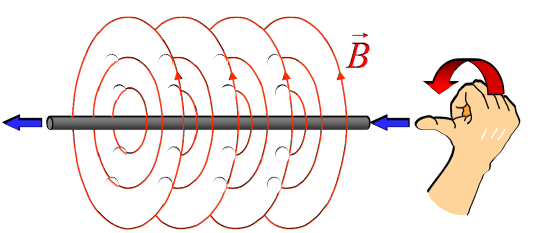
\includegraphics[width=4cm]{magneto/image0.png}
\captionof{figure}{Règle de la main droite}
\end{wrapfigure}

Le fait que la boussole tourne d'un sens et pas dans l'autre met en avant un \textit{problème de brisure de symétrie} qui à beaucoup préoccupé à l'époque. C'est en cherchant à résoudre ce problème qu'Ampère définissa la \textit{règle de la main droite} pour anticiper le sens du courant.

\subsection{Formule de Biot et Savart}
Ceux-ci découvrirent le lien de proportionnalité (expérimentalement, par la prise de mesures systématiques) entre le champ $B$ et $\frac{I}{r}$ grâce aux moments de forces.

\subsection{Interactions entre courants}
Si un courant provoque une force sur un aimant alors forcément l'aimant provoque une force sur le courant (conservation de l'énergie\footnote{Les courants inter-réagissent entre eux.}).\\\\
On peut en déduire que les courants interagissent entre eux et donc :
\begin{enumerate}
\item Si \textit{I} va dans le même sens, il y aura attraction entre ces fils
\item Si \textit{I} va dans le sens opposé, il y aura répulsion entre ces fils
\end{enumerate}
\ 


Pour en arriver à ces conclusions, Ampère a regarder la force magnétique d'un fil $B$ provoquée par un courant dans le fil $A$. (Notons que la force magnétique n'a pas la même direction que le champ qui la génère, elle lui est orthogonale)
\\
On a donc :
\begin{equation}
\Vert \vec{F_M} \Vert\ \propto\ l \frac{I_1 I_2}{d}
\end{equation}
\begin{comment}
\subsection{Courant dans un champ uniforme}
Considérons un fil passant entre l'entrefer d'un aimant afin de le placer dans un champ magnétique uniforme. En mesurant le module du champ, on remarque que $\vec{F_M}\ \perp\ \vec{1_x}\ \Rightarrow\ \vec{F_M}\ \propto\ I.l.B$.\\
De cette proportionnalité, par convention, on définit l'égalité suivante : $ \vec{F_M}\ \equiv Ilb$ où $[B] = \frac{N}{A.m} = T$\\

\textit{NB :} C'est cette convention qui fixe la définition du Tesla donnée ci-dessus.
\begin{center}
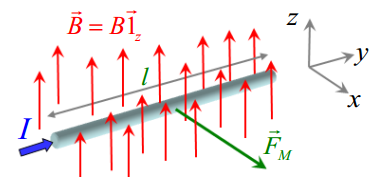
\includegraphics[scale=0.55]{magneto/image1.png}
\captionof{figure}{Fil électrique dans un champ magnétique}
\end{center}
Si le fil possède une inclinaison $\theta$ ($\neq \frac{\pi}{2}$), on remarque expérimentalement que la direction de la force magnétique reste \textbf{inchangée} mais que son module est proportionnel au sinus de l'angle : $\vec{F_M} = I.l.B.\sin(\theta)$.
\\

Introduisons un produit vectoriel pour rendre ceci compact. Sachant que $I = S.||\vec{J}||$ où $S$ est la section du fil (on fait apparaître un vecteur). \\
En introduisant le produit vectoriel (équivalent à la norme des deux vecteurs que multiplie le sinus de l'angle entre les deux), on peut écrire : 
\begin{equation}
\fbox{$\vec{F_M} = l.S.\vec{J} \times \vec{B} $}
\end{equation}

Ce qui respecte bien sur la règle de la main droite.

\subsection{Force de Lorentz}
Histoire que l'électrostatique nous serve à quelque chose, on l'introduit ici :
$\vec{F_M} =  l.S.\vec{J} \times \vec{B}$ et $\vec{J} =  \eta q \vec{v}$ (\textit{Rappel  : $I = \frac{\Delta q}{\Delta t}$ et $\delta q = \eta_c q_e v \delta t S$}.) 
\begin{center}
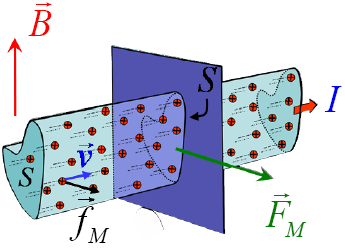
\includegraphics[scale=0.55]{magneto/image4.png}
\captionof{figure}{Électrostatique - Définition du courant}
\end{center}
En remplaçant l'un dans l'autre :
\begin{equation}
\vec{F_M} = \underbrace{lS\eta_c}_{N_e} q_e \vec{v} \times \vec{B} = N_eq \vec{v} \times \vec{B}
\end{equation}

Le $N_e$ (nombre de particules chargées) dans la dernière égalité nous montre que $F_M$ est la \textbf{somme} des forces magnétiques \textbf{individuelles} exercée sur chacune des particules ayant une vitesse $\vec{v}$. On appellera ainsi la \textit{force de Lorentz} la force magnétique \textbf{individuelle} :
\begin{equation}
\fbox{$f_M = q \vec{v} \times \vec{B} $}
\end{equation}

On peut conclure que le champ magnétique est responsable d'une force sur les charges en mouvement (si les charges n'étaient pas liées au fil, elles s'en iraient!).\\


\textit{NB : } Si un champ électrique $\vec{E}$ est présent en même temps, la force totale est simplement la somme de la force électrique et magnétique.

\textit{NB2 :} Cette force ne dépend pas du signe de la charge, le déplacements des électrons étant inverse au sens du courant. ($\vec{f_M} = (-q_e)(-\vec{v})\times \vec{B} = q_e \vec{v} \times \vec{B}$) \\

\subsection{Particule libre dans un champ uniforme}
Etudions le cas ou la particule n'est plus liée à un matériel conducteur (une charge dans un champ B par exemple).
\begin{center}
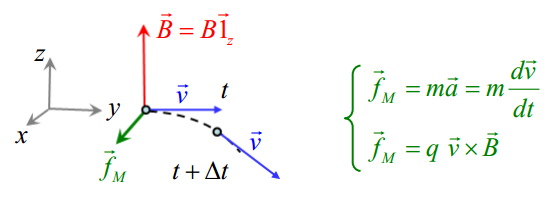
\includegraphics[scale=0.75]{magneto/image2.png}
\captionof{figure}{Rayon de courbure (1)}
\end{center}
\begin{wrapfigure}[15]{l}{4cm}
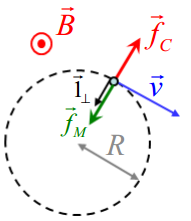
\includegraphics[width=4cm]{magneto/image3.png}
\captionof{figure}{Rayon de courbure (2)}
\end{wrapfigure}
L'égalité des deux expressions ci-dessus, multipliée de part et d'autre par $\vec{v}$ vaut zéro. Ceci est du que le produit vectoriel de $\vec{v}$ donne un vecteur perpendiculaire à lui-même (et donc le produit scalaire de ce nouveau vecteur sera nul). Ceci implique que \textit{la vitesse est constante}.

C'est du au fait que la force de Lorentz est à tout moment perpendiculaire à la vitesse de la particule, et donc à la trajectoire de celle-ci (le vecteur vitesse étant partout tangent à la trajectoire ($\vec{dl} = \vec{v}dl$) et donc cette force ne peut effectuer de travail (seulement possible si $\exists$ composante non nulle dans la direction du déplacement) $\Rightarrow$ pas de $W$, pas de $\Delta E_c$, pas de variation du module de la vitesse.\\


Comme la vitesse est constante, le déplacement décrit une trajectoire circulaire (si la vitesse ne varie pas, le module de $\vec{F}_m$ non plus $\Rightarrow$ force appliquée à la particule toujours perpendiculaire à la vitesse de celle-ci $\Rightarrow$ impose une courbure à la trajectoire). Comme la force centrifuge vaut $\frac{-mv^2}{R}\vec{1_\perp}$ et que nous savons que $\vec{f_m} + \vec{F_c} = 0$, on peut trouver le \textit{rayon de courbure :}
\begin{equation}
\fbox{$R = \frac{mV}{qB}$} 
\end{equation}


\subsection{Relation entre champ et courant : La perméabilité}
\textit{But :} Quantifier le champ magnétique par un courant donné.\\
Comme on sait que $\Vert \vec{B} \Vert \propto \frac{I}{r}$, on introduit un vecteur de proportionnalité $\frac{\mu_0}{2\pi}$ où $\mu_0$ est la \textit{perméabilité du vide}, une constante fondamentale de la nature reliant le courant électrique au champ magnétique qu'il produit.\\

Ampère, par mesures successives étudia la force subie par un fil $B$ du au champ magnétique généré par un fil $A$. Les deux fils étant parallèles, on peut utiliser la formule du champ uniforme : $||\vec{F_M}|| = I l ||\vec{B}||$. En remplaçant dans cette expression la \textit{formule} de Biot et Savart :
\begin{equation}
||\vec{F_M}|| = I_Bl\frac{\mu_0}{2\pi}\frac{I_A}{r}
\end{equation}




Par convention, la force entre les deux fils, avec $I_A = I_B = 1\ A, l = r = 1\ m$ vaut $10^{-7}\ N$. On dès lors trouve la constante recherchée :
\begin{equation}
[\mu_0] = \frac{T.m}{A} = 4\pi . 10^{-7}
\end{equation}

Le $4\pi$ est du au choix de l'unité de courant, l'ampère.\footnote{Le $C$ >> $T$, parce que les effet magnétiques sont très faibles par rapport aux effets électriques.}

\section{Loi d'Ampère}
Comme Gauss pour l'électrostatique, Ampère formula une loi équivalente pour la magnéto-statique.
\subsection{Circulation de champ magnétique}
Calculons l'intégrale de circulation du champ magnétique sur une trajectoire circulaire centrée sur le courant qui génère le champ. Le schéma ci-dessus montre  que le champ est orienté en $\vec{1_\theta}$ (vecteur unitaire polaire), nous permettant d'écrire : $\vec{B} = \frac{\mu_0 I}{2\pi r}\vec{1_\theta}$
\begin{center}
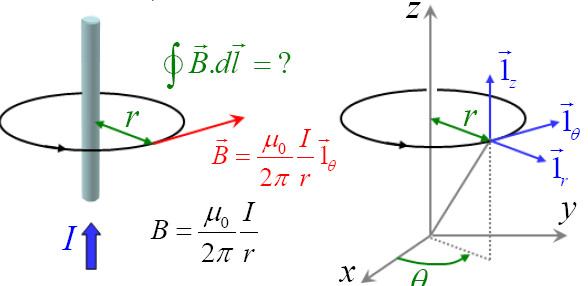
\includegraphics[scale=0.65]{magneto/image5.png}
\captionof{figure}{Circulation du champ magnétique}
\end{center}

C'est simple à calculer, la trajectoire étant une ligne de champ. \textit{Confond} nous apprend qu'il faut effectuer le produit $\vec{B}.\vec{dl}$. Cet accroissement $\vec{dl}$ vaut ici $rd\theta\vec{1_\theta}$. Le produit scalaire couplé à la formule de Biot et Savart nous donne :
\begin{equation}
\vec{B}.\vec{dl} = (B.\vec{1_\theta}).(rd\theta\vec{1_\theta}) = Brd\theta = \frac{\mu_0 I}{2\pi} d\theta
\end{equation}

En intégrant sur tout le contour, soit un angle de $2\pi$, il nous reste simplement $\mu_0 I$.
\begin{equation}
\oint \vec{B}.\vec{dl} = \int_0^{2\pi} \frac{\mu_0 I}{2\pi} d\theta = \mu_0 I
\end{equation}


\subsubsection*{Trajectoire fermée quelconque}
La trajectoire n'étant pas circulaire, il faut tenir compte de l'angle entre $\vec{B}$ et $\vec{dl}$. Nous sommes ici contraint à utiliser un vecteur déplacement généraliser : $\vec{dl} = dr \vec{1_r} + rd\theta \vec{1_\theta} + dz \vec{1_z}$. \\

Mais pas de panique, le champ étant orienté en $\vec{1_\theta}$ seule la composante polaire sera prise en compte ce qui nous ramène au cas étudié ci-dessus. 
La loi d'Ampère généralisée s'exprime ainsi :
\begin{equation}
\fbox{$\oint \vec{B}.\vec{dl} = \mu_0 I$}
\end{equation}


\subsection{Trajectoire ouverte}
Le raisonnement est identique à celui suivi précédemment si ce n'est que de passer de $0$ à $2\pi$ on intègrera de $\theta_i$ à $\theta_f$ :
\begin{equation}
\int_{i\rightarrow f} \vec{B}.\vec{dl} = \frac{\mu_0}{2\pi}I\Delta\theta
\end{equation}


\subsubsection{Courant extérieur}
On va dans un sens, puis dans l'autre ! Le résultat est logique :
\begin{equation}
\oint \vec{B}.\vec{dl} = 0
\end{equation}

Il faut donc que ce que l'on appellera plus tard le \textit{chemin ampérien} entoure la source de courant.

\subsubsection{Principe de superposition}
Également d'application en magnéto, il permet de généraliser la Loi d'Ampère à plusieurs courant.
\begin{equation}
\oint \vec{B}.\vec{dl} = \mu_0 \sum_{n=1}^N I_n
\end{equation}

Il faut tenir compte du sens du courant : si le sens de circulation correspond au sens opposé à celui de la main droite, alors il doit être considéré comme négatif.

\section{Loi de Biot \& Savart}
Ampère ne nous permet en réalité que de calculer l'expression du champ magnétique dans des configurations de courant particulières. La \textbf{Loi} deBiot \& Savart a été obtenue expérimentalement et permet de calculer le champ magnétique \textit{en un point} dans des configurations \textit{non symétrique}. Biot et Savart ont calculé le champ magnétique en une multitude de points sans trouver de relation. 

\begin{wrapfigure}[15]{r}{4cm}
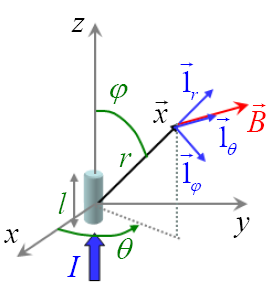
\includegraphics[scale=0.55]{magneto/image6.png}
\captionof{figure}{Système de coordonnée sphérique}
\end{wrapfigure}

C'est Pierre-Simon Laplace qui a réussi à en trouver une en se basant sur un système de coordonnées sphériques. En gros, il a 'vu' cette  horreur : $ ||\vec{B}|| \propto Il sin\phi / r^2$. Il remarqua aussi la présence d'un coefficient de proportionnalité valant $\frac{\mu_0}{4\pi}$.
%\begin{center}
%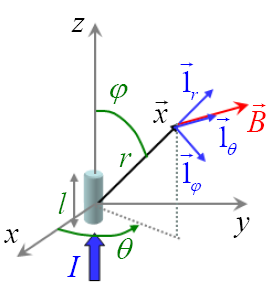
\includegraphics[scale=0.55]{magneto/image6.png}
%\end{center}



Pour introduire une notation compacte, sachant que le champ est dirigé en $\vec{1_\theta}$ et vu la présence d'un sinus, on peut réécrire $sin\phi \vec{1_\theta}$ en $\vec{1_z} \times \vec{1_r}$. En introduisant le fait que le fil de courant est orienté en $\vec{1_z}$ on peut formuler la \textbf{Loi de Biot et Savart} sous sa forme intégrale :
\begin{equation}
d\vec{B} = \frac{\mu_0}{4\pi r^2}I\vec{dl} \times \vec{1_r}
\end{equation}

ou encore sous sa forme intégrale :
\begin{equation}
\fbox{$\vec{B} = \frac{\mu_0 I}{4\pi} \int \frac{1}{r^2}\vec{dl} \times \vec{1_r}$}
\end{equation}


\section{Calculs de champs magnétiques}
\subsection{Application de la loi d'Ampère}
\subsubsection{Le fil rectiligne}
Tentons de retrouver la formule de B\&S en partant de notre brave relation fraichement découverte.\\

Choisissons un contour Ampérien circulaire centré sur le fil. Ce dernier ayant une symétrie de révolution, il ne peut être \textbf{fonction} de la coordonnée polaire, ni même de la coordonnée en $z$, le fil étant supposé infini.


Il faut trouver maintenant la \textbf{direction} du champ (que nous avons justement oubliée). Si l'on procède à l'intégrale de circulation $\int_C \vec{B}.\vec{dl}$\footnote{$\vec{dl} = dr.\vec{1_r}$}, l'ouverture $\Delta\theta$ sera nul $\Rightarrow$ le champ sera nul $\Rightarrow$ $\vec{B}.\vec{1_r} 0 = \Rightarrow \vec{B} \perp \vec{1_r}$.\\


Un raisonnement similaire peut être tenu avec l'axe $z$ impliquant $\vec{B}.\vec{1_z} = 0$. Par élimination, le champ ne peut qu'être orienté selon le vecteur unitaire polaire : $\vec{B} = B(r).\vec{1_\theta}$. Comme $\vec{dl} = rd\theta\vec{1_\theta}$ le résultat est immédiat :
\begin{equation}
\oint_C Brd\theta = \mu_0 I \Leftrightarrow rB2\pi = \mu_0 I \Rightarrow B = \frac{\mu_0}{2\pi}\frac{I}{r}
\end{equation}



\subsubsection{La "paroi de courant"}
Une paroi de courant est une rangée plane de fils conducteurs transportant tous le même courant $I_0$. Ampère nous permet de calculer fil par fil pour ensuite utiliser le principe de superposition et calculer toute la plaque.

\begin{center}
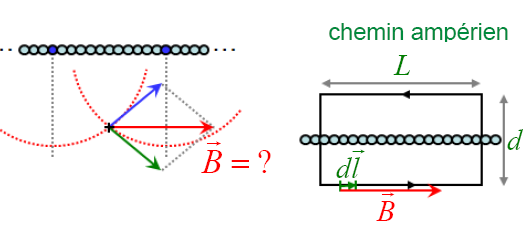
\includegraphics[scale=0.55]{magneto/image7.png}
\captionof{figure}{Chemin ampérien}
\end{center}


Par symétrie, il apparaît évident que le champ est en tout point parallèle à la plaque. On choisira dès lors un contour ampérien qui est soit parallèle ($\vec{B}.\vec{dl} = Bdl$) au champ, soit perpendiculaire à celui-ci ($\vec{B}.\vec{dl} = 0$). \\
La longueur d'un côté parallèle au champ vaut L, le produit scalaire vaudra $BL$. Comme une plaque possède deux côtés (Sisi !), on a $2BL$ et ensuite, ce n'est plus que formalité ! 
\begin{equation}
\oint_C \vec{B}.\vec{dl} = \mu_0I \Leftrightarrow 2BL = \mu_0N I_0
\end{equation}

En faisant apparaître la notion de \textit{densité surfacique de courant}, c'est à dire le courant par unité de longueur transversant la paroi, soit $J_S = \frac{NI_0}{L}$ on trouve le module du champ généré par la paroi.
\begin{equation}
\fbox{$B = \frac{1}{2}\mu_0J_S$}
\end{equation}

\textit{NB :} Ce n'est le champ que d'un côté de la plaque !

\subsection{Application de la Loi de Biot et Savart}
Quand la configuration est trop complexe pour être traitée par la loi d'ampère, on utilisera B\&S.

\subsubsection{Champ au centre d'une spire}
(Notons avant tout que les calculs se font dans le cas ou $z$ est l'axe perpendiculaire au plan de la spire)
La difficulté de cette loi est de rendre son intégrale calculable. Pour le vecteur $\vec{dl}$, considérons la spire comme  un cercle. Ce vecteur vaudra ainsi $Rd\theta\vec{1_\theta}$. 

\begin{wrapfigure}[12]{r}{4cm}
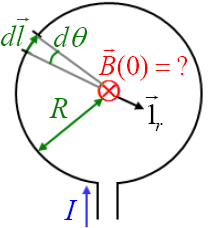
\includegraphics[scale=0.55]{magneto/image8.png}
\captionof{figure}{Champ au centre d'une spire}
\end{wrapfigure}


Ces deux vecteurs étant perpendiculaire, leur produit vectoriel se calcule simplement : $\vec{dl} \times \vec{1_r} = Rd\theta\vec{1_z}$. Il reste donc à intégrer le résultat qui suit :
\begin{equation}
d\vec{B}(0) = \frac{\mu_0}{4\pi R^2}IRd\theta\vec{1_z}
\end{equation}

Comme tout est constant à l'exception de $d\theta$, tout peut sortir de l'intégrale et le résultat de l'intégrale vaut $2\pi$. Le champ au centre d'une spire peut ainsi être calculé.
\begin{equation}
\vec{B}(0) = \frac{\mu_0 I}{2R}\vec{1_z}
\end{equation}

\textit{NB :} On peut voir le vecteur $\vec{1_r}$ comme le vecteur \textit{pointant vers  notre œil}. En gros, il pointe vers le point ou on veut calculer le champ.

\subsubsection{Champ sur l'axe d'une spire}
Tout comme précédemment, $\vec{dl} \perp \vec{1_r}$, le produit vectoriel se calcul aisément ; $||d\vec{B}|| = \frac{\mu_0 I}{4\pi r^2}dl$.\\
La spire étant centrée, on peut toujours s'arranger pour obtenir un champ orienté le long de l'axe $z$ comme suggérer sur le schéma ci-dessous.

\begin{center}
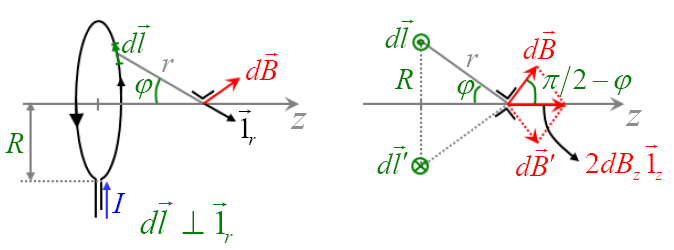
\includegraphics[scale=0.70]{magneto/image9.png}
\captionof{figure}{Champ sur l'axe d'une spire}
\end{center}



Comme une paire d'éléments de longueur diamétralement opposée génère un champ de $2dB_z\vec{1_z}$, le champ magnétique total sera également en $\vec{1_z}$. Comme le montre le schéma, ce petit champ infinitésimal $d\vec{B}$ fait un angle de $\frac{\pi}{2} - \phi$ entre le vecteur unitaire radial $\vec{1_r}$ et l'axe $z$.\\

Cet angle représente une sorte d'\textit{ouverture angulaire} dont il faut tenir compte en multipliant le résultat obtenu ci-dessus par le cosinus de cet angle.
\begin{equation}
dB_z = \frac{\mu_0}{2\pi r^2}Idl\sin (\phi)
\end{equation}

Comme $dl = Rd\theta$ et que $\theta$ varie de $0 \rightarrow 2\pi$, on peut calculer le champ générer par une spire sur l'axe $z$.
\begin{equation}
B = \frac{\mu_0}{2 r^2} IR \sin (\phi)
\end{equation}

Il ne nous reste qu'à nous débarrasser de $r$ (à ne \textbf{pas} confondre avec R!) en nous servant de notre trigonométrie de base : $r.\sin (\phi) = R$.
\begin{equation}
\vec{B} = \frac{\mu_0}{2R}I \sin^3(\phi)\vec{1_z}
\end{equation}


Comme on pouvait s'en douter, le champ est maximal au centre de la spire, lorsque l'ouverture vaut 90 degrés. Quand on s'éloigne, le champ suit malheureusement pour lui une décroissance en $\sin^3\phi$.\\

\begin{wrapfigure}[9]{l}{4cm}
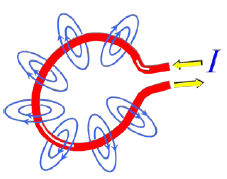
\includegraphics[scale=0.50]{magneto/image10.png}
\captionof{figure}{Représentation intuitive}
\end{wrapfigure}

Calculer le champ d'une spire en tout point de l'espace est trop complexe, on peut néanmoins se faire une idée intuitive en se basant sur le schéma ci-contre.


\subsubsection{Le solénoïde}
Il s'agit "simplement" d'un ensemble de spire parallèles parcourues par le même courant. Pour calculer le champ, utilisons le champ généré par une spire (trouvé un peu plus haut) et utiliser le principe de superposition.\\

Plaçons la spire en $z = z'$. Si le point de calcul est repérée par l'ordonnée $z$, on peut en déduire une relation remarquable liant $z'$ à $\phi$ : $R = (z - z')tan(\phi)$.

\begin{center}
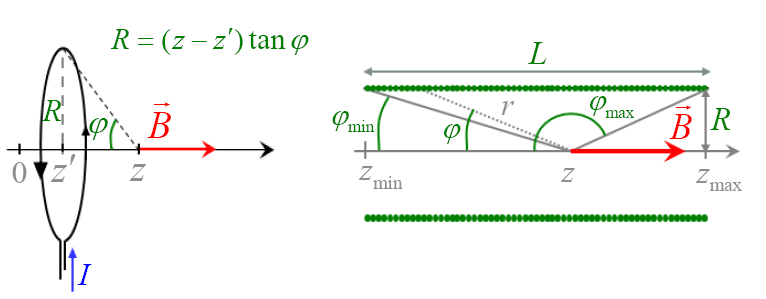
\includegraphics[scale=0.70]{magneto/image11.png}
\captionof{figure}{Calcul du champ du solénoïde}
\end{center}

Pour calculer le champ, on va considérer que le solénoïde contient un grand nombre de spires très serrées caractérisée par une densité linéique de spires notée $e$. Ainsi, un élément de longueur $dz'$ contient $ndz'$ spires.\\

Le champ total est alors donné par la sommes sur $z'$ du début du solénoïde ($z' = z_{min}$) jusqu'à la fin ($z' = z_{max}$).
\begin{equation}
B(z) = \frac{\mu_0 nI}{2R}\int \sin^3\phi dz'
\end{equation}

Cette intégrale n'est pas calculable. Il faut procéder à un changement de variable pour ré-exprimer $dz'$ en fonction de $\phi$. Nous effectuons les opérations suivantes :
\begin{itemize}
\item $z - z' = \frac{R}{tg(\phi)} = Rcotg(\phi)$
\item $-dz' = R\frac{d}{d\phi}[cotg(\phi)]d\phi$
\item $dz' = \frac{R}{sin^2(\phi)}d\phi$
\end{itemize}
Ce qui nous donne :
\begin{equation}
B(z) = \frac{\mu_0 nI}{2}\int_{\phi_{min}}^{\phi^{max}} \sin\phi d\phi
\end{equation}

Pas besoin d'aide pour calculer l'intégrale, celle ci vaut (où $cos(\phi_{max}) = cos(\pi - \phi_{max})$) : 
\begin{equation}
B(z) = \frac{\mu_0 nI}{2}[cos(\phi_{min}) - cos(\pi - \phi_{max})]
\end{equation}

L'interprétation physique est immédiate  : quand on se situe à un point \textit{éloigné} $\rightarrow \phi_{max} = \pi$ et donc le champ est nul. Alors que si on se trouve au centre, $\rightarrow \phi_{min} = \frac{\pi}{2}$\\ \\
\emph{Milieu du solénoïde}\\\\
Le point centre du solénoïde se caractérise par l'égalité $\phi_{min} = \pi - \phi_{max}$ de sorte qu'on puisse exprimer le champ tel que : $B = \mu_0nIcos(\phi_{min})$\\

On remarque à partir de cette relation que plus $L >> R$, plus l'angle va tendre vers zéro, et donc, le champ tendra à devenir maximal. Lorsque la condition $L >> R$, on se trouve dans un \textit{solénoïde idéal} (c'est à dire arbitrairement long par rapport à son rayon de sorte que l'on puisse condidérer que $\phi_{min} = 0$ et $\pi - \phi_{max} = 0$ pour tous ses points intérieurs, sauf tout près de ses extrémités) dont le champ interne vaut  :
\begin{equation}
B_{int} = \mu_0nI\footnote{Le $n$ est bien la densité linéique de spire !}
\end{equation}

\emph{Extrémité du solénoïde}\\\\
A l'extrémité gauche, au niveau de la spire d'entrée du solénoïde idéal, $\phi_{min} = \frac{\pi}{2} \Rightarrow B = \frac{1}{2}\mu_0nIcos(\pi - \phi_{max})$. Le soso étant considérer idéal ; $\pi - \phi_{max} = 0$. On appellera $B_{ext}$ le champ aux extrémités pour rappeler ce fait.
\begin{equation}
\fbox{$B_{ext} = \frac{1}{2}\mu_0nI$}
\end{equation}


\begin{center}
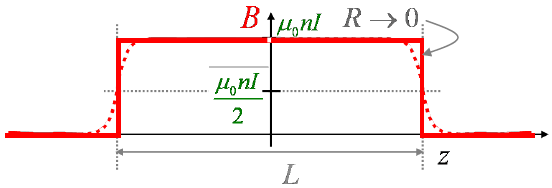
\includegraphics[scale=0.60]{magneto/image12.png}
\captionof{figure}{Extrémité du solénoïde}
\end{center}

Introduisons la notion de \textit{densité de courant de surface}. Sachant que le nombre $N$ de fils est donné par $\frac{\Delta z}{d}$ où $d$ est le diamètre du fil. Le courant total correspond à cette expression multipliée par $I$. En divisant par la longueur qu'il occupe, soit $\Delta z$, on obtiens la densité de courant de surface du solénoïde : $J_S = \frac{NI}{\Delta z} = nI$.

\begin{equation}
\fbox{$B_{int} = \mu_0J_S$}
\end{equation}

\subsubsection{Interprétation des propriétés magnétiques de la matière}
Une lecture attentive des pages $53 - 56$ devrait suffire !

\section{Couple de force sur une spire de courant}
Un aimant plongé dans un champ subit un moment de force qui tend à l'aligner avec de champ. C'est le moment de le calculer ! \\
Le schéma ci-dessous représente une spire de courant plongée dans un champ magnétique uniforme avec un angle non nul et ses côtés verticaux perpendiculaire au champ.
\begin{center}
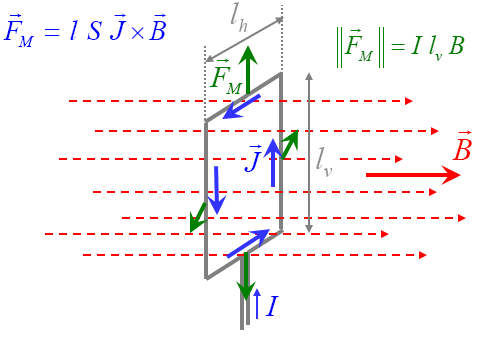
\includegraphics[scale=0.50]{magneto/image13.png}
\captionof{figure}{Couple de force sur une spire de courant}
\end{center}

Les forces magnétiques (en vert) des côtés horizontaux s'annulent, mais ce n'est pas le cas des deux autres (elles n'ont en effet pas le même support).\\

\begin{wrapfigure}[13]{l}{4cm}
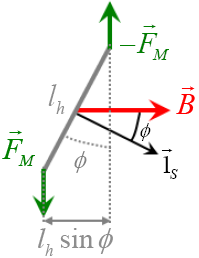
\includegraphics[scale=0.50]{magneto/image14.png}
\captionof{figure}{Calcul du moment de force}
\end{wrapfigure}

\textit{Confond} nous apprend que le moment se calcule en multipliant la force par le bras de levier. Dans notre cas, il faut tenir compte de l'angle $\phi$ présent entre $\vec{B}$ et $\vec{1_S}$.\\



Le moment calculé vaut donc : $\tau = ||\vec{F_M}||l_h sin\phi$ ou en remplaçant la force magnétique par sa valeur on trouve : $\tau = I l_v B l_h sin\phi$.\\
En introduisant la surface de la spire $ S = l_v l_h$ on a :
\begin{equation}
\fbox{$\tau = ISBsin\phi$}
\end{equation}

Cette formule est valable pour une surface quelconque. Il suffit d'imaginer pleins de spires rectangulaires élémentaires. Les côtés tangents aux spires verront leurs courants devenir nul et ne restera que les courants de surfaces.
\subsection{Moment magnétique dipolaire}
Le moment est une grandeur vectorielle, généralisons l'expression en une expression vectorielle en faisant disparaître le sinus grâce à un... produit vectoriel !
\begin{equation}
\fbox{$\tau = IS\vec{1_S} \times \vec{B}$}
\end{equation}
On appellera le facteur $IS\vec{1_S}$ le moment magnétique noté $\vec{m_M}$ de la sorte que l'on puisse écrire $\tau = \vec{m_M} \times \vec{B}$.

\subsection{Champ magnétique dans la matière}
\subsubsection{Paramagnétisme}
Les électrons s'associent par paires opposées causant l'annulation du moment magnétique. Mais parfois, leur nombre est impair et il se crée alors un moment magnétique. Si l'on plonge un tel matériau dans un champ magnétiques, les atomes vont s'aligner au champ et subir une \textit{magnétisation}.\\
\\
En gros : \textit{"Les matériaux paramagnétiques sont les matériaux dans lesquels le phénomène d'alignement induit par un champ magnétique extérieur se produit en compétition avec l'agitation thermique".} En effet, l'agitation thermique peut empêcher l'alignement des atomes et donc leur magnétisation.\\

Le matériel aimanté peut être vu comme un aimant (un ensemble de spires générant des courants de surfaces) générant un \textit{champ magnétique induit} $\vec{B_i}$ qui va s'ajouter au champ initial $B_0$ pour former le champ total (on somme les deux). Pour exprimer ceci, on utilise généralement la perméabilité relative $\mu_r = \frac{\mu}{\mu_0}$. Logiquement, celle-ci est toujours supérieur à l'unité pour les matériaux paramagnétiques.\\

\textit{NB :} Ici, contrairement à l'électrostatique, les deux champs vont dans le même sens expliquant la présence de $\mu_0$ au numérateur.

\subsubsection{Ferromagnétisme}
Certains atomes ayant un nombre impair d'électrons ont des propriétés $\neq$ du aux interactions entre les moments magnétiques des atomes voisins.  Cela conduit à un alignement spontané des moments magnétiques ou certains "domaines" du matériau "reçoivent" une aimantation permanente.\\

\textit{Un matériau est ferromagnétique si certaines parties deviennent des aimants même après avoir retiré $\vec{B}$.} Ici, l'agitation thermique ne suffit plus pour désorienter les moments magnétiques.

\subsubsection{Le moteur à courant continu}
Encore une fois, une bonne lecture suffit ! (\textit{Cf. page 69 - 71})

\section{Forme locale de la loi d'Ampère}
La difficulté des lois d'Ampères et de B\&S vient du fait qu'elles sont non-locales : le champ est calculé à une certaine distance des courants. Existe-t-il une loi locale liant $\vec{B}$ et $I$ \textbf{au même} point ?

\subsection{Distribution de courant continue}
\begin{wrapfigure}[7]{l}{4cm}
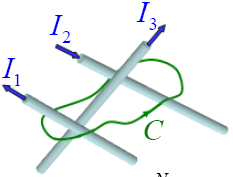
\includegraphics[scale=0.50]{magneto/image15.png}
\captionof{figure}{Densité de courant}
\end{wrapfigure}

La loi d'Ampère développée quelques pages avant ne s'applique qu'aux courants dans les fils. Pour la généraliser, on va préférer la notation de densité de courant $\vec{J}$.\\





On définit une \textit{surface sous-tendue par le contour} C avec laquelle on va calculer le flux.
\begin{equation}
\oint \vec{B}.\vec{dl} = \mu_0 \int_{S_C} \vec{J}.\vec{dS}
\end{equation}


\subsection{Contour élémentaire}
Considérons une distribution de courant continue ou $\vec{J}(\vec{x})$ est la valeur de la distribution au point $\vec{x}$. On va appliquer Ampère à un contour élémentaire autour de $\vec{x}$. Prenons-en un dans le plan $y-z \rightarrow \perp \vec{1_x}$ (d'ou le contour $C_x$ (\textit{cf. ci-dessous}).
\begin{center}
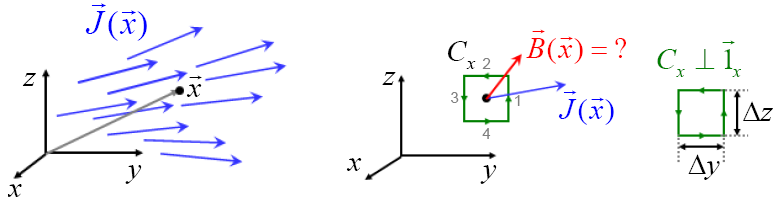
\includegraphics[scale=0.60]{magneto/image16.png}
\captionof{figure}{Choix d'un contour élémentaire}
\end{center}
La loi d'Ampère pour ce contour vaut : 
\begin{equation}
\oint_{C_x} \vec{B}.\vec{dl} = \mu_0\int_{\Delta S} \vec{J}d\vec{S}
\end{equation}

Calculons le membre de droite. Comme $C_x \rightarrow 0 \Rightarrow \vec{J}(x) = cste$ ; on peut le sortir de l'intégrale. Cette dernière ne contient que $\vec{dS}$ ce qui nous donne $\Delta \vec{S} = \Delta y\Delta z \vec{1_x}$.
\begin{equation}
\oint_{C_x} \vec{B}.\vec{dl} = \mu_0J_x \Delta y\Delta z
\end{equation}

Calculons maintenant le champ grâce au contour ampérien :
\begin{equation}
\oint \vec{B}.\vec{dl} = \int \vec{B}.\vec{dl}_1 + \int \vec{B}.\vec{dl}_2 + \int \vec{B}.\vec{dl}_3 + \int \vec{B}.\vec{dl}_4 = \mu_0J_x \Delta y\Delta z
\end{equation}

Commençons par les côtés 1 et 3.\\
Comme $\vec{dl}_1 \parallel \vec{1_z}$, le produit scalaire $\vec{B}.\vec{dl}_1$ fait apparaître la composante en $z$ du champ magnétique :
\begin{equation}
\vec{B}.\vec{dl}_1 = B_z(x, y + \frac{\Delta y}{2}, z')dz'
\end{equation}

\begin{center}
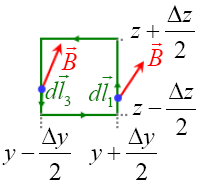
\includegraphics[scale=0.60]{magneto/image17.png}\\
\captionof{figure}{Circulation le long d'un contour élémentaire}
\end{center}
En suivant le même raisonnement avec le côté 3
\begin{equation}
\vec{B}.\vec{dl}_3 = -B_z(x, y - \frac{\Delta y}{2}, z')dz'
\end{equation}

Plutôt que de garder z', considérons la largeur $\Delta z$ ; C'est identique comme nous somme dans le cas d'un accroissement infinitésimal. Le schéma suivant l'explicite bien :
\begin{center}
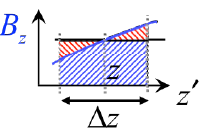
\includegraphics[scale=0.60]{magneto/image18.png}\\
\captionof{figure}{Approximation de la surface}
\end{center}

\textbf{Attention :} le passage de $z' \rightarrow z$ ne signifie pas que $z$ ne varie pas !\\

En sommant les deux expressions et en multipliant par $\frac{\Delta y}{\Delta y}$ :
\begin{equation}
\int \vec{B}.\vec{dl}_1 + \int \vec{B}.\vec{dl}_3 = [\frac{B_z(x, y + \frac{\Delta y}{2}, z)  - B_z(x, y - \frac{\Delta y}{2}, z)]}{\Delta y}\Delta z\Delta y
\end{equation}

Ce qui correspond à la dérivée partielle de $B_Z$ par rapport à $y$. Autrement dit :
\begin{equation}
\int \vec{B}.\vec{dl}_1 + \int \vec{B}.\vec{dl}_3 = \frac{\partial B_z}{\partial y}\Delta y\Delta z
\end{equation}


En suivant un raisonnement similaire pour le côté 2 et 4 :
\begin{equation}
\int \vec{B}.\vec{dl}_2 + \int \vec{B}.\vec{dl}_4 = -\frac{\partial B_y}{\partial z}\Delta y\Delta z
\end{equation}


En sommant le tout :
\begin{equation}
\oint_{C_x} \vec{B}.\vec{dl} = [\frac{\partial B_z}{\partial y} - \frac{\partial B_y}{\partial z}]\Delta y\Delta z = \mu_0J_x\Delta y\Delta z
\end{equation}


Ce qui donne après simplification :
\begin{equation}
\frac{\partial B_z}{\partial y} - \frac{\partial B_y}{\partial z}= \mu_0J_x
\end{equation}


\subsection{Loi d'Ampère locale}
On peut faire les mêmes raisonnements pour $C_y$ et $C_z$ :
\begin{center}
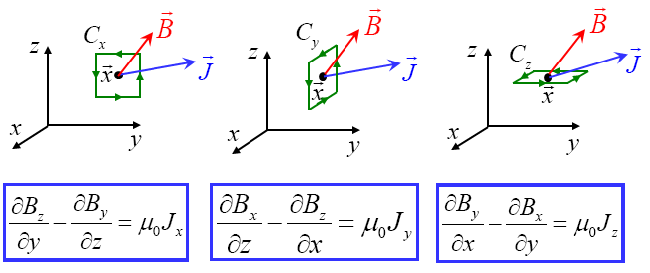
\includegraphics[scale=0.70]{magneto/image19.png}\\
\captionof{figure}{Loi d'Ampère locale}
\end{center}
En regardant la symétrie, on remarque que celle-ci est identique à celle du produit $\vec{A} \times \vec{B}$ où $\vec{A} = \vec{\nabla}$ (le fameux opérateur nabla)\\
\begin{equation}
\fbox{$Loi\ d'Ampère\ locale\ \ \ \ \ :\ \ \ \vec{\nabla} \times \vec{B} = \mu_0\vec{J}$}
\end{equation}


\subsection{Le rotationnel}
$\vec{\nabla} \times$ est un opérateur vectoriel nommé \textit{rotationnel} $\Rightarrow rot\ \vec{B} = \mu_0\vec{J}$.\\
Le terme \textit{rot} rappelle que les composantes du rotationnel d'un champ vectoriel sont obtenues par le calcul de la circulation de ce camp sur les contours fermés infinitésimaux.

\subsection{Interprétation du rotationnel}
En nous basant sur $C_x$ :
\begin{equation}
\oint_{C_x} \vec{B}.\vec{dl} = rot\ \vec{B}\vec{1_x}\Delta S_x \Rightarrow rot\ \vec{B}\vec{1_x} = \frac{\oint_{C_x} \vec{B}.\vec{dl}}{\Delta S_x}
\end{equation}

La composante en $x$ du rot est donc l'intégrale de circulation d'un contour élémentaire perpendiculaire à l'axe $x$ divise par la surface sous-tendue à ce contour.\\
\textit{Circulation normalisée par la surface sous-tendue le contour $C_x$}.

\subsection{Généralisation }
Facilement généralisable en changeant de repère et en repérant l'orientation de la surface élémentaire par le vecteur $\vec{1_{C_x}}$.\\

En faisant tendre $\Delta S_{C_x} \rightarrow 0$, cela revient à prendre la norme du rot multiplié par le cosinus de l'angle entre ce dernier et $\vec{1_{C_x}}$. (On voit que si l'angle est nul, on est au maximum. Tout le reste est toujours inférieur)\\

En conclusion, le rot en $\vec{x}$ est la circulation normalisée \textbf{la plus grande} que l'on puisse avoir au point $\vec{x}$ pour toute les orientations possibles. De plus, le rot pointe dans la direction de la circulation la plus grande. 

\section{Théorèmes d'analyse vectorielle}
\subsection{Théorème de Stokes}
Considérons la loi d'Ampères : $\oint_C \vec{B}.\vec{dl} = \mu_0 \int_{S_c} \vec{J}.\vec{dS}$ et l'expression du rotationnel : $rot\ \vec{B} = \mu_0\vec{J}$. En isolant $\vec{J}$ dans la seconde expression et en l'injectant dans la première :
\begin{equation}
\oint_C \vec{B}.\vec{dl} = \int_{S_C} rot\ \vec{B}.\vec{dS}
\end{equation}

\textit{Le flux du rot $\vec{B}$ au travers de la surface $S_C$ sous tendue par le contour $C$ est égale à l'intégrale de circulation de $\vec{B}$ sur ce contour.}\\
La généralisation (Pour une fonction vectorielle $\vec{F}$ est le \textbf{Théorème de Stokes :}
\begin{equation}
\oint_C \vec{F}.\vec{dl} = \int_{S_C} rot\ \vec{F}.\vec{dS}
\end{equation}


\subsection{Théorème d'Ostrogradski}
Théorème se rapportant à la divergence d'un champ vectoriel. Connaissant l'expression de la loi de Gauss : $\oint_S \vec{E}.d\vec{S} = \frac{1}{\epsilon_0} \int \rho(\vec{x})dV$ et son expression locale : $div.\vec{E} = \frac{1}{\epsilon_0}\rho(\vec{x})$. En remplaçant l'une dans l'autre : 
\begin{equation}
\oint_S \vec{E}.d\vec{S} = \int_{V_S} div.\vec{E}\ dV
\end{equation}

\textit{Le flux du champ électrique à travers d'une surface $S$ vaut l'intégrale de volume de sa divergence sur tout le volume $V_S$ enfermé par la surface $S$ est égale à l'intégrale de circulation de $\vec{B}$ sur ce contour.}\\

La généralisation (Pour une fonction vectorielle $\vec{F}$ est le \textbf{Théorème d'Ostrogradski :}
\begin{equation}
\oint_S \vec{F}.d\vec{S} = \int_{V_S} div.\vec{F}\ dV
\end{equation}

\subsection{Illustrations}
\subsubsection{Rotationnel du champ électrostatique}
Soit $\vec{E}$ et son potentiel $V \rightarrow \Delta V = - \int_i^f \vec{E}.\vec{dl}$. Or, sur un contour fermé, le potentiel est nul $\Rightarrow \oint \vec{E}.\vec{dl} \equiv 0$.\\

Or selon le Th. de Stokes : $\oint_C \vec{F}.\vec{dl} = \int_{S_C} rot\ \vec{F}.\vec{dS} \Rightarrow rot\ \vec{E} = \vec{0}$, c'est à dire que le champ est conservatif (\textit{Cf. méca}).

\subsubsection{Rotationnel d'un gradient}
Comme rot $\vec{E} = \vec{0}$ et $E = - grad\ V \Rightarrow rot\ \vec{E} = -rot[grad\ V] = \vec{0}$.\\
Ainsi, pour toute fonction vectorielle $\vec{F} : rot(grad(\vec{F})) = \vec{0}$

\subsubsection{Divergence du rotationnel}
Appliquons le Th. de Stokes à un contour ferme $C$ dont la longueur tend vers zéro.\\
$\lim\limits_{\substack{C \to 0}} \oint_C \vec{F}.\vec{dl} = \int_{S_C} rot\ \vec{F} d\vec{S} = 0 \Rightarrow$ Le Th. de Stokes nous indique que le flux du rot de $\vec{F}$ au travers de tout surface fermée $S$ est nul.\\
Appliquons le Th. d'Ostrogradski à $\vec{G}$ où $\vec{G} = rot\ \vec{F}$ :
\begin{equation}
\oint_S rot\ \vec{F}d\vec{S} = \int_{V_S} div(rot\ \vec{F})dV = 0\ \ \ (\forall\ \ V_S)\ \ \ \Rightarrow div[rot\ \vec{F}(\vec{x})] \equiv 0
\end{equation}


\section{Divergence du champ magnétique}
Considérons un élément de courant élémentaire véhiculant un courant $I$. La loi de Bios \& Savart nous informe que $\vec{B} = \frac{\mu_0}{4\pi r^2}I\Delta l\ \vec{1_l} \times \vec{1_r}$. Considérons une surface $S$ délimitant un \textit{tube de flux} représenté ci-dessus vu d'ensemble et vu du  haut.
\begin{center}
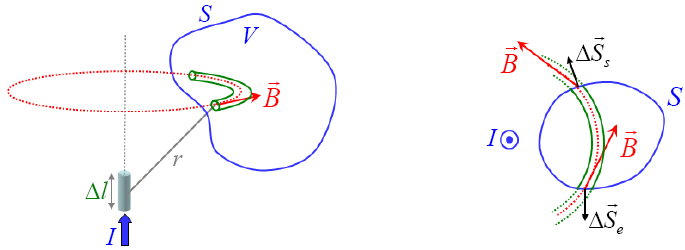
\includegraphics[scale=0.60]{magneto/image20.png}\\
\captionof{figure}{Divergence du champ magnétique - Courant extérieur}
\end{center}
Le flux d'entrée et de sortie sont égaux en valeur absolue. On peut exprimer l'équilibre de la façon suivante : $\vec{B}.\Delta\vec{S}_e + \vec{B}.\Delta\vec{S}_s = 0$.\\

Imaginons que l'espace soit découpé d'un ensemble de $N$ tubes: $\sum_{n=1}^N [\vec{B}.\Delta\vec{S}_e + \vec{B}.\Delta\vec{S}_s] = 0$. En passant à la limite infinitésimale, j'ai bien : $\oint_S \vec{B}.\vec{dS} = 0$. On en conclus qu'un \textbf{flux de champ magnétique sur une surface fermée extérieure est toujours nulle}.\\

Si on considère un élément de courant intérieur, certaines lignes de champ n'interceptent pas la surface et ne participent donc pas au flux. D'autres l'interceptent en sortant mais quand elles l'intercepte à nouveau pour rentrer, le flux s'annule.
\begin{center}
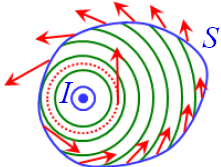
\includegraphics[scale=0.60]{magneto/image21.png}\\
\captionof{figure}{Divergence du champ magnétique - Courant intérieur}
\end{center}
$\Rightarrow \oint_C \vec{B}.\vec{dS} = 0$. Appliquons le Th. d'Ostrogradski :
\begin{equation}
\oint_S \vec{B}.d\vec{S} = \int_{V_S} div.\vec{B}\ dV = 0
\end{equation}

En faisant tendre $V_S \rightarrow 0$, la divergence peut être considérer comme constante et sortir de l'intégrale. Il ne reste plus que l'intégrale de $dV$ qui tend vers 0. (Considérons pour la ligne ci-dessus que $V_S \rightarrow 0$)
\begin{equation}
\int_{V_S} div\ \vec{B}dV = div\ \vec{B}\int_{V_S} dV = div\ \vec{B} V_S = 0
\end{equation}
\begin{equation}
\fbox{$div\ \vec{B} = 0 $}
\end{equation}
\\

Ce résultat est généralisable en sommant les $\vec{B}$ élémentaires.
















































\chapter{Électromagnétisme}
\section{Introduction}
Discipline scientifique décrivant les systèmes de charges électriques dans les situations les plus générales de charges et de courants variables.

\subsection{La dynamo}
Soit un courant en déplacement dans un champ magnétique uniforme $\vec{B}$ (par exemple, un fil effectuant une translation de vitesse $\vec{v}$. Les charges (considérons les positives) vont ainsi subir une force de Lorentz ($q\vec{v} \times \vec{B}$)orientée dans l'axe du fil causant la migration des charges libres transversalement.
\begin{center}
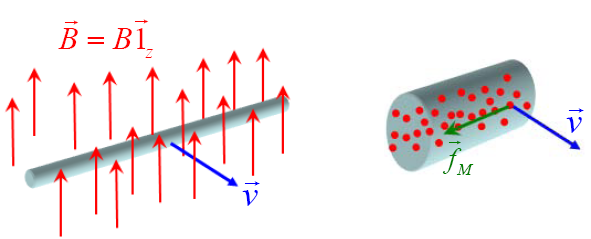
\includegraphics[scale=0.35]{em/image0.png}\\
\captionof{figure}{Fil plongé dans un champ magnétique uniforme}
\end{center}
La migrations des charges provoque une accumulation de charges positives dans le bas de la tiges mais aussi un défaut de charge positives sur la partie supérieure qui se charge négativement $\Rightarrow$ génération d'un champ électrostatique $\vec{E}_S$ dirigé vers le haut, s'opposant à la migration des charges (de par la force de Lorentz) créant un potentiel entre les extrémités. (\textbf{Attention !} Remarque \textit{page 3})
\begin{center}
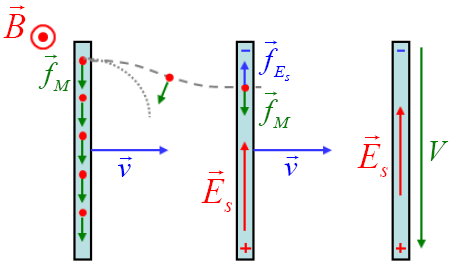
\includegraphics[scale=0.55]{em/image1.png}\\
\captionof{figure}{Apparition de la force de Lorentz}
\end{center}
Ceci a été découvert expérimentalement par Faraday, qui inventa d'ailleurs la dynamo.\\

Le principe est de mettre un disque en rotation dans l'entrefer d'un aimant $\Rightarrow$ Forces de Lorentz $\Rightarrow$ Migration des charges $\Rightarrow$ Différence de potentiel établie $\Rightarrow$ Crée une source de tension.

\subsection{Force électromotrice}
Calculer le champ électrostatique $\vec{E}_S$ est simple : Sachant que $\vec{f_{E_S}} + \vec{F_M} = 0$ ($q\vec{E}_S + q\vec{v}\times \vec{B}$), on trouve $\vec{E}_S = -\vec{v} \times \vec{B}$.\\
Or, de par la géométrie du problème $\vec{v} \perp \vec{B} \Rightarrow ||\vec{v} \times \vec{B}|| = vB$. Si le fil est de longueur $l$, $V$ se trouve facilement.
\begin{equation}
\fbox{$Force\ électromotrice\ \equiv V = lvB $}
\end{equation}

\textit{NB :} Cette force n'est \textbf{pas} en Newton ! \textit{Electromotrice} traduit le fait que l'on est dans un mécanisme de séparation de charges.

\section{L'induction électromagnétique}
\subsection{Relativité galiléenne et force de Lorentz}
La relativité Galiléenne stipule que tout référentiel inertiel sont équivalents, ce qui n'est pas vérifié ici (particule au repos ou le champ magnétique se déplace à vitesse $-\vec{v}$)(En effet, il n'y a pas de raison de dire que c'est la tige qui bouge et non l'aimant.)\\
Dans une telle configuration, la vitesse de la particule est nulle, la force de Lorentz doit l'être aussi ($\vec{f}_m = q\vec{v}\times\vec{B}\ où\ \vec{v} = \vec{0}$) $\Rightarrow$ contradiction avec ce qui est dit ci-dessus.\\

Pour régler le problème, on introduit une nouvelle force, identique à celle de Lorentz mais non magnétique ($\vec{v} = \vec{0}$). $\vec{B}$ étant en mouvement, cette force serait du au mouvement, au "balayement" des lignes de champ "créant" cette nouvelle force. Faraday propose l'apparition d'un champ électrique induit.
\begin{center}
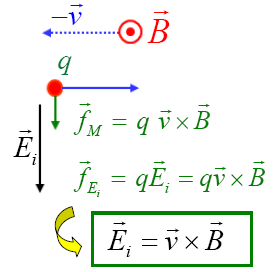
\includegraphics[scale=0.55]{em/image2.png}\\
\captionof{figure}{Calcul du champ induit}
\end{center}
Une charge électrique au repos dans une zone ou $\vec{B}$ est en mouvement suivra une force électrique remplaçant la force de Lorentz (son expression rappelle d'ailleurs cette dernière)
\begin{equation}
\fbox{$ Champ\ électrique\ induit\ \equiv \vec{E_i} = \vec{v} \times \vec{B}$}
\end{equation}

Le phénomène de balayage des lignes de champ est appelé \textit{induction électromagnétique}.\\
\textbf{Attention !} Le champ électrique induit n'est pas généré par des
charges électriques en tant que telles mais bien par un mouvement de champ
magnétique.

\subsection{Induction et force électromotrice}
Considérons une tige fixe véhiculant du courant et un aimant bougeant à la vitesse $^-\vec{v}$. Ci dessous, l'image de cette tige balayée par les lignes de champ magnétiques ; \textit{La ou je 'balaye', j'ai ce champ électrique induit qui apparait.}
\begin{center}
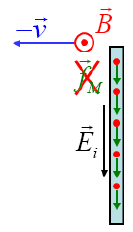
\includegraphics[scale=0.35]{em/image3.png}\\
\end{center}
La tige étant au repos, la vitesse des particules $\vec{v_c}$ l'est aussi ; la force de Lorentz également. \\

Pour résoudre ce 'souci Galiléen', Faraday proposa sous forme de conjecture qu'un balayement des lignes champ créait un champ induit provoquant une force électrique induite $\vec{f}_{E_i}$ remplaçant $\vec{f}_M$ (dirigée dans le sens de $\vec{E}_i$, ici vers le bas).
\begin{center}
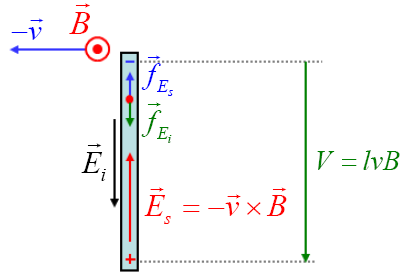
\includegraphics[scale=0.45]{em/image4.png}\\
\captionof{figure}{Potentiel non-nul}
\end{center}

\subsection{Comparaison avec l'influence électrostatique}
Il est important de ne \textbf{pas} confondre champ induit et champ électrostatique.
\subsubsection*{Influence électrostatique}
Dans cette situation, $\vec{E_i}$ est du à la présence de charges de part et d'autre de la tige (séparation du au champ extérieur $\vec{E}_s$), provoquant une migration des charges libres jusqu'à ce que le champ électrique total soit nul (champ toujours dans un conducteur (apparition d'un champ opposé induit, ...).
\begin{center}
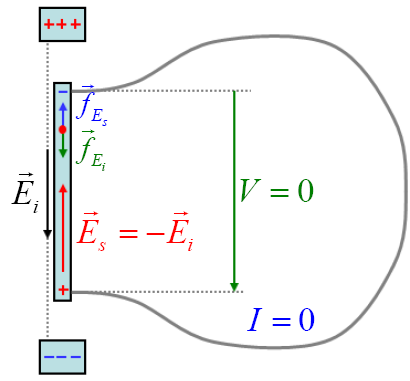
\includegraphics[scale=0.45]{em/image5.png}\\
\captionof{figure}{Influence électrostatique}
\end{center}
Comme on se trouve à l'équilibre $\Delta V = 0$. Rappelons aussi que $\vec{E} = \vec{E_i} + \vec{E_s} = \vec{0}$ (sinon on aurait violation de la conservation de l'énergie).\\
Ces deux champs étant tous deux \textit{électrique}, ça explique la d.d.p. nulle.

\subsubsection*{Induction électromagnétique}
Ici le champ électrostatique est en opposition au champ induit est responsable d'un potentiel valant $lvB$. 
\begin{center}
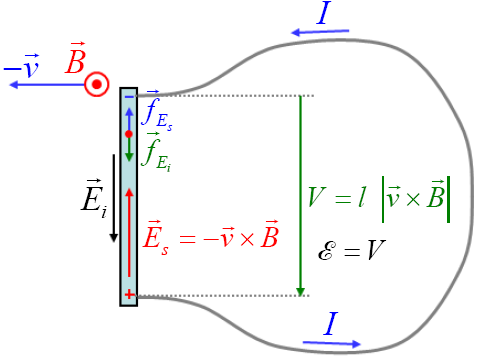
\includegraphics[scale=0.45]{em/image6.png}\\
\captionof{figure}{Induction électromagnétique}
\end{center}
Si ici $"\Delta V" \neq 0$ c'est parce qu'on ne prend en compte \textbf{que les champs électriques ce qui n'est pas le cas de $\vec{E}_i$}.\\
Quand on se trouve en situation de courant variable, la notion de potentiel électrique n'a qu'un sens très limité, juste à la composante électrostatique.\\
Pour re-donner un sens à tout cela, on va définir comme la \textbf{force électromotrice} le potentiel $V$ correspondant à $\vec{E_S}$ seul. Ce dernier valant $-\vec{E_i}$ dans un conducteur à l'équilibre nous donne l'expression de la force électromotrice :
\begin{equation}
\fbox{$ \xi \equiv \int_i^f \vec{E}_i.\vec{dl}$}
\end{equation}

Physiquement, cela illustre que c'est à cause de $\vec{E}_i$ que les charges se déplaceront.

\subsection{Variations temporelles du champ magnétique}
L'augmentation du courant rend le champ magnétique plus important : l'environnement devient plus dense en ligne de champ. On dira que ces "nouvelles" lignes de champ se déplace, comme ci-dessus, à vitesse $-\vec{v}$ provoquant un champ électrique induit $\vec{E}_i = \vec{v} \times \vec{B}$.
\begin{center}
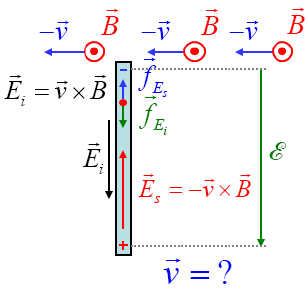
\includegraphics[scale=0.45]{em/image7.png}\\
\captionof{figure}{Déplacement du champ magnétique $\vec B$}
\end{center}
Le schéma ci-dessus représente la situation vue localement. Une autre expression pour $\xi$ peut ainsi être :
\begin{equation}
\xi \equiv \int_i^f \vec{v} \times \vec{B}.\vec{dl}
\end{equation}


\textit{NB :} j'insiste encore une fois sur le fait que $\vec{E}_i = \vec{v} \times \vec{B}$ mais que le champ nous intéressant dans la force électromotrice, $\xi$ vaut $-\vec{v} \times \vec{B}$.


\section{Spires et induction}
Connaître la vitesse des lignes de champ n'est pas réalisable, il va falloir ruser.

\subsection{Champ homogène}
Imaginons une spire carrée se déplaçant dans un champ à la vitesse $\vec{v}$, causant un déplacement des lignes de champ en $-\vec{v}$. 
\begin{center}
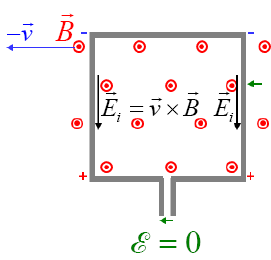
\includegraphics[scale=0.45]{em/image8.png}\\
\captionof{figure}{Spire carrée se déplaçant dans un champ homogène}
\end{center}
Sur les côtés horizontaux, $\vec{f_m}$ est dirigée vers le bas mais les charges ne se déplacement pas le long du conducteur, donc pas de force électromotrice.\\

La force de Lorentz étant parallèle aux côtés verticaux, on aura une force électromotrice non-nulle mais celle-ci étant équivalente des deux côtés, $xi = 0$.
\begin{center}
\textit{Pas de force électromotrice accumulée sur un tour complet de la spire, quelque soit le point d'où on part pour faire ce tour.}
\end{center}
\begin{equation}
\xi \equiv \oint_C \vec{E}_i.\vec{dl} = \oint_C \vec{v} \times \vec{B}.\vec{dl} = 0
\end{equation}


\subsection{Champ inhomogène}
Même situation que la sous-section précédente sauf que le champ n'étant pas homogène, la densité de ligne de champ diffère d'un endroit à l'autre, causant une $\xi$ plus grande.
\begin{center}
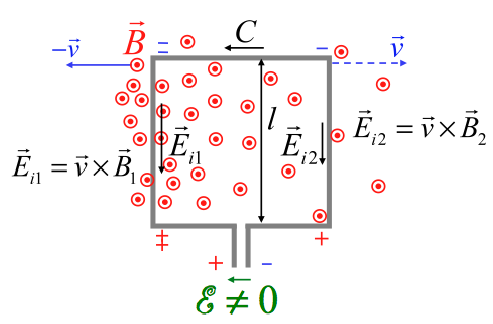
\includegraphics[scale=0.45]{em/image9.png}\\
\captionof{figure}{Spire carrée se déplaçant dans un champ non-homogène}
\end{center}
La force électromotrice totale sera $\neq 0$ et se calcule simplement : $\xi = l(||\vec{E}_{i1}|| - ||\vec{E}_{i2}|| = lv(B_1 - B_2)$.\\

\subsection{Variations du flux magnétique : loi d'induction de Faraday}
On peut exprimer $\xi$ en fonction du flux de champ magnétique. Prenons encore une fois la situation précédente (vitesse spire $\vec{v}$, lignes de champ $-\vec{v}$, ...).\\
L'astuce de Faraday est d'exprimer sa loi en terme du \textit{flux de champ magnétique} sous-tendu à la surface $S_C$
\begin{equation}
\Phi_M = \int_{S_C} \vec{B}.d\vec{S}
\end{equation}

L'induction n'a lieu que si le champ varie : logique de considérer les variation du flux. Pour se faire, considérons un petit temps $dt$ durant laquelle la spire s'est déplacée de $vdt$.

\begin{center}
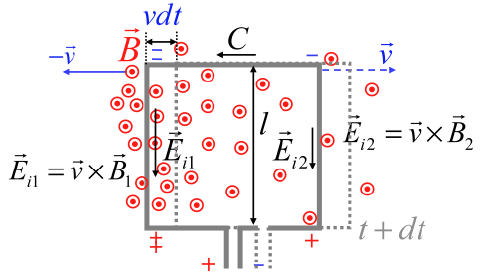
\includegraphics[scale=0.45]{em/image10.png}\\
\captionof{figure}{Évolution temporelle du flux}
\end{center}
Si \textbf{seul le côté gauche} était en mouvement (spire déformable), la surface diminuerait et forcément $\Phi_M$ aussi : diminution de $-lvdt$ sur le temps $dt$ ($l$ = largeur de la spire). Ensuite les lignes de champ "arrivent" aux deuxième côté qui lui engendrerait une augmentation (on imagine maintenant que seul ce côté bouge). \\
En sommant les deux variations : 
\begin{equation}
d\Phi_M = -lvdtB_1 + lvdtB_2
\end{equation}

En divisant les deux membres par $dt$, on obtient l'opposée de $\xi$ calculée plus haut (\textit{section 3.2})
\begin{equation}
\frac{d\Phi_M}{dt} = -lvB_1 + lvB_2 = - \xi
\end{equation}

Ce qui nous donne la loi de Faraday pour une spire carrée en  mouvement...
\begin{equation}
\xi = \oint_C \vec{E}_i.\vec{dl} = - \frac{d\Phi_M}{dt}
\end{equation}

\textit{NB :} Le mouvement de la tige vers la gauche crée une force magnétique vers le bas, poussant les charges + vers le bas ce qui signifie que le gradient du potentiel électrique induit est dirigé dans le sens opposé au sens de parcours de la spire. Le potentiel croît en descendant la tige mobile. Cette signification physique justifie le signe négatif. 
\begin{center}
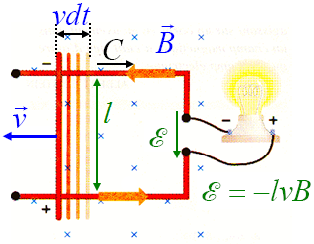
\includegraphics[scale=0.45]{em/image11.png}\\
\captionof{figure}{Exemple concret}
\end{center}
\textit{Une variation positive de flux magnétique engendre un champ électrique induit dirigé dans le sens opposé au sens de parcours conventionnel (donné par la règle de la main avec le pouce dans le sens du champ magnétique).}

\subsection{Généralisation : contour quelconque}
Considérons une situation encore une fois similaire au précédente, mais cette fois-ci avec une spire de forme quelconque.
\begin{center}
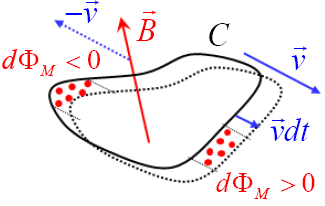
\includegraphics[scale=0.45]{em/image12.png}\\
\captionof{figure}{Spire au contour quelconque}
\end{center}
Le flux au temps $t$ :
\begin{equation}
\Phi_M(t)= \int_{S_C(t)} \vec{B}.d\vec{S}
\end{equation}

\textit{Wiki : Il s'agit du flux de $\vec{B}$ à travers d'une surface orientée sous tendue à un contour $C$}.
Au temps $t+dt$ :
\begin{equation}
\Phi_M(t+dt)= \int_{S_C(t+dt)} \vec{B}.d\vec{S}
\end{equation}

On peut voit le flux au temps $t+dt$ comme le flux au temps $t$ additionné d'un petit flux infinitésimal : $\Phi_M(t+dt) : \Phi_M(t) + d\Phi_M(t)$.\\

A certains endroits, le balayage des lignes de champ provoque une augmentation du flux alors qu'à travers d'autre, c'est une diminution du flux. 
\begin{equation}
\Phi_M(t+dt) = \int_{S_C(t)} \vec{B}.d\vec{S} + \int_{dS_C} \vec{B}.d\vec{S}
\end{equation}

\begin{center}
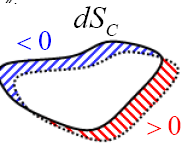
\includegraphics[scale=0.45]{em/image29.png}\\
\captionof{figure}{Variation du flux de la spire}
\end{center}
Mais encore : 
\begin{equation}
\Phi_M(t+dt) = \Phi_M + \int_{dS_C} \vec{B}.d\vec{S}
\end{equation}


Ce qui nous permet de faire apparaître la \textit{surface différence} $dS_C$, c'est à dire la variation de surface entre $t$ et $t+dt$.

A la limite infinitésimale, une portion du contour va devenir un élément $\vec{dl}$. La somme de ceux-ci définissent le coutour $C$ et donc cette surface différence.

\begin{equation}
d\Phi_M = \Phi_M(t+dt) - \Phi_M(t) = \int_{dS_C} \vec{B}.d\vec{S}
\end{equation}

Il faut maintenant faire en sorte qu'un agrandissement de la surface engendre un flux > 0 en choisissant un vecteur surface adapté.\\

La surface à considérer est celle engendrée par le déplacement de la spire. La surface balayée par un élément $\vec{dl}$ est donnée par l'aire du parallélogramme construit sur les vecteurs $\vec{v}dt$ et $\vec{dl}$ ce qui peux s'exprimer comme $\vec{v}dt \times \vec{dl}$ soit $vdtdlsin\theta$.
\begin{center}
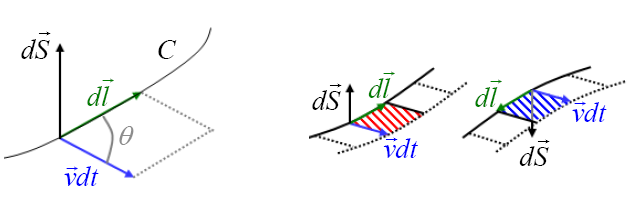
\includegraphics[scale=0.45]{em/image13.png}\\
\captionof{figure}{Vecteur surface}
\end{center}
On peut ré-exprimer en explicitant $d\vec{S}$ :
\begin{equation}
d\Phi_M = \int_{dS_C} \vec{B}.d\vec{S} = \oint_C \vec{B}.(\vec{v}dt \times \vec{dl})
\end{equation}

On obtient une $\oint$ comparable à une intégrale de circulation dans le sens ou la somme se fait sur les éléments de longueur $\vec{dl}$ sur toute la longueur du contour $C$ de la spire. \\

On va sommer les éléments $\vec{dl}$ sur le contour $C$ et notre expression du vecteur surface tiendra compte naturellement des flux entrants et sortants.\\
En divisant par $dt$ :
\begin{equation}
\frac{d\Phi_M}{dt} = \oint_C \vec{B}.(\vec{v} \times \vec{dl})
\end{equation}


Connaissant la règle du produit mixte ($\vec{A}.(\vec{B}\times\vec{C}) = -(\vec{B}\times\vec{A}).\vec{C}$), on peut ré-écrire cette expression et faire apparaître le champ induit :
\begin{equation}
\frac{d\Phi_M}{dt} = -\oint_C (\vec{v} \times \vec{B}).\vec{dl} = -\oint_C \vec{E}_i.\vec{dl}
\end{equation}

On en déduit la loi de Faraday appliquée au cas ou des spires sont en mouvement dans un champ magnétique stationnaire.
\begin{equation}
\frac{d\Phi_M}{dt} = -\oint_C \vec{E}_i.\vec{dl}
\end{equation}
Que l'on peut ré-écrire en introduisant la définition du flux magnétique et en tant compte que $S_C(t)$ est la seule chose variant dans le temps.
\begin{equation}
\fbox{$ oint_{C(t)} \vec{E}_i.\vec{dl} = -\frac{d}{dt}\int_{S_C(t)} \vec{B}.\vec{dS}$}\
\end{equation}

\subsection{Généralisation : contour déformable}
Facilement généralisable, il suffit de tenir en compte les variations spatiales et temporelles de la vitesse.

\subsection{Généralisation : champ variable}
Aussi d'application quand \textbf{seul} $\vec{B}$ varie. On considèrera simplement la vitesse $-\vec{v}$ du au lignes de champ, le résultat en découlera.\\
\textbf{Loi d'induction de Faraday}
\begin{equation}
\oint_{C(t)} \vec{E}_i(\vec{x}, t).\vec{dl} = -\frac{d}{dt}\int_{S_C(t)} \vec{B}(\vec{x}, t).d\vec{S}
\end{equation}
\textit{NB :} Les développements ci-dessus ont été réalisé en prenant $d\vec{S}$ dans le même sens que $\vec{B}$. Si ce n'est pas le cas, il faut se baser sur la règle de la main droite.

\subsubsection*{Illustrations}
Dans un solénoïde, quand le courant augmente, le champ magnétique augmente également $\Rightarrow$ augmentation de la densité de lignes de champ à vitesse $\vec{-v}$ (en bleu) provoquant un champ induit $\vec{E}_i$.\\
Si la spire est bien sur l'axe du solénoïde, une augmentation du courant dans ce dernier augmente le champ à l'intérieur. Les lignes "traversent" la spire et viennent se resserrer au milieu expliquant la vitesse $-\vec{v}$ (champ de plus en plus fort, de plus en plus de lignes 'entrent' et se resserrent).
\begin{center}
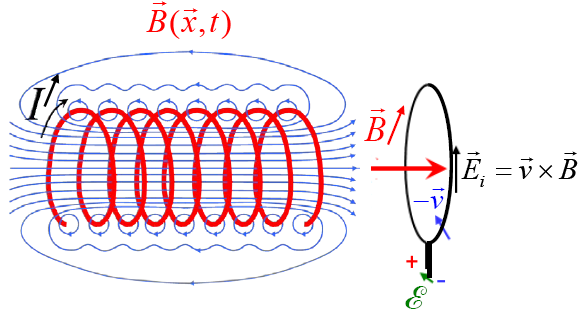
\includegraphics[scale=0.45]{em/image14.png}\\
\captionof{figure}{Flux au travers d'un solénoïde}
\end{center}
Le champ induit est dirigé dans le sens opposé de parcours (règle main droite) provoquant l'apparition d'un courant opposé. Il y a accumulation de charge des deux côtés de la borne à laquelle on connecte une résistance pour que le courant puisse passer.La spire fonctionne ainsi comme un générateur au même titre qu'une pile.

\begin{center}
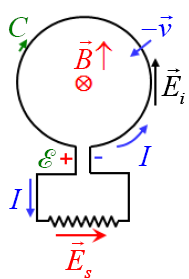
\includegraphics[scale=0.45]{em/image15.png}\\
\captionof{figure}{Ressèrement des lignes de champ}
\end{center}

\section{Forme locale de la loi d'induction}
On peut localiser la loi grâce au Th. de Stokes (qui contient la def du rot (ORAL)). Il faut d'abord comprendre que le champ $\vec{E}_i$ qui apparaît dans la loi de Faraday ne nécessite pas la présence d'une spire pour exister mais a tout objet balayé par des lignes de champ. Par Stokes :
\begin{equation}
\oint_C \vec{E}_i.\vec{dl} = \int_{S_C} rot\ \vec{E}_i.d\vec{S} = -\frac{d}{dt}\int_{S_C} \vec{B}.d\vec{S}
\end{equation}
(Le - se justifie par dS dans le sens du pouce et dl dans le sens des doigts)
\\
Notons qu'ici $S_C$ désigne une surface ouverte, les bords constituant le contour $C$.
En considérant une surface $\Delta S$ arbitrairement petite : 
\begin{equation}
rot\ \vec{E}_i.\Delta\vec{S} = -\frac{\partial \vec{B}}{\partial t}.\Delta\vec{S}
\end{equation}

Ces deux surfaces étant identique, on obtient la loi locale de Faraday :
\begin{equation}
rot\ \vec{E}_i = -\frac{\partial \vec{B}}{\partial t}
\end{equation}

\subsection{Généralisation}
Cette expression ne se rapporte qu'au champ électrique induit $\vec{E}_i$, apparaissant lors de variations de champ magnétique. 
\begin{center}
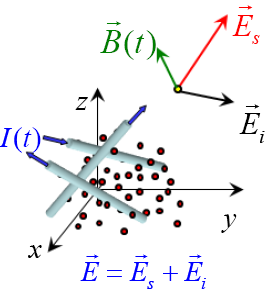
\includegraphics[scale=0.45]{em/image16.png}\\
\captionof{figure}{Champ électrostatique et induit}
\end{center}
S'il y a présence de charges électrique au sein d'un système électromagnétique, il y aura un champ électrique $\vec{E}_S$ en plus du champ induit.\\
Sachant que $rot\ \underbrace{\vec{E}_S = 0}_{conservatif}$ et $rot\ \vec{E}_i = -\frac{\partial \vec{B}}{\partial t}$, on peut écrire :
\begin{equation}
rot\ \vec{E} = rot(\vec{E}_S + \vec{E}_i) = -\frac{\partial \vec{B}}{\partial t}
\end{equation}
On en conclus que la loi de Faraday locale est valable pour le champ électrique total.
\begin{equation}
\fbox{$rot\ \vec{E} = -\frac{\partial \vec{B}}{\partial t}$}
\end{equation}

\section{Loi de Lenz}
\subsection{Opposition du champ induit}
Comme la vitesse de balayement des ligne de champ vaut $-\vec{v}$ (cadre magnétostatique) on crée un champ induit $\vec{E}_i$ créant forcément un courant induit $I-i$ allant de $+ \rightarrow -$. Ce courant pousse les charge jusqu'à la résistance pour créer un petit dipôle et générer un champ $\vec{E}_S$ si le circuit est fermé.\\
Mais encore mieux : le courant induit $I_i$ crée un champ magnétique induit $\vec{B}_i$ \textbf{s'opposant à la variation de }$\vec{B}$.

\begin{center}
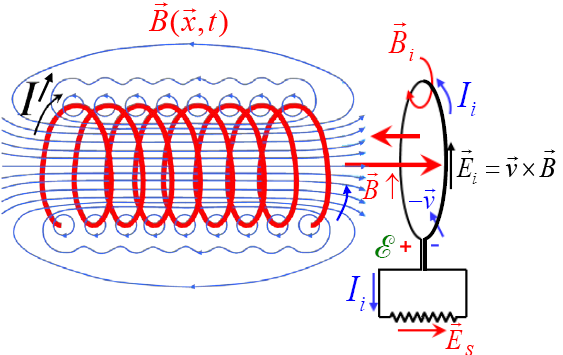
\includegraphics[scale=0.55]{em/image17.png}\\
\captionof{figure}{Flux au travers d'un solénoïde}
\end{center}
\textbf{Loi de Lenz :} le champ magnétique induit par la spire est opposé à la variation du champ extérieur $\vec{B}$.\\
Si le champ diminue, $I_i$ sera dans la même sens que $I \Rightarrow \vec{F}_M$ attractive pour "compenser" la diminution de $\vec{B}$.

\subsection{Conservation de l'énergie}
Quand un aimant est éloigné de la spire, il apparaît une force attractive si la spire est fermée sur un circuit. $\vec{B}_i$ va aller dans le même sens que $\vec{B}$ pour compenser sa diminution.
\begin{center}
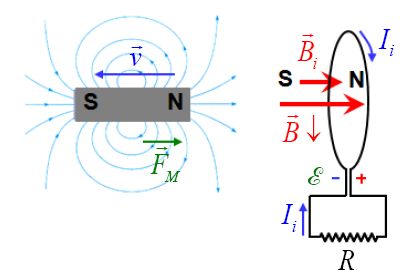
\includegraphics[scale=0.45]{em/image18.png}\\
\captionof{figure}{Représentation de la conservation d'énergie}
\end{center}
Le fait que les deux aimants s'attirent va créer une $F_M$ : il faudra dès lors appliquer une puissance mécanique pour déplacer l'aimant qui peut facilement s'exprimer.
\begin{equation}
P = RI_i^2 = \frac{\xi^2}{R} = -\vec{F}_M.\vec{v}
\end{equation}
Ici la puissance sera dissipée à travers la résistance, le retrait de l'aimant dissipe la puissance dans la spire.

\section{Champ magnétique dans la matière}
\subsection{Diamagnétisme}
Observable seulement sur des matériaux ni ferromagnétiques, ni paramagnétiques $\Rightarrow$ il faut un nombre pair d'$e^-$ ($\vec{m}_M = 0$).\\
Considérons un atome avec un électron décrivant une boucle : spire microscopique. Si l'on rapproche un aimant, on va diminuer la vitesse orbitale de celui-ci. Comme le nombre d'$e^-$ est pair, il n'est jamais seul : Un autre $e^-$ va tourner dans l'autre sens mais ici la vitesse orbitale va augmenter $\Rightarrow$ induction responsable d'un déséquilibre de courant entre orbites. Cette deuxième orbite possédant un courant plus élevé fait que $\vec{B}_i$ sera opposé à $\vec{B}$.\\

Une fois que l'aimant aura fini de bouger, le phénomène d'induction s'arrête ($\vec{E}_i = \vec{0}$) mais $\vec{B}_i$ reste tant que le champ magnétique extérieur reste stationnaire.\\

\textit{NB :} Si la spire n'était pas macroscopique, il  n'y aurait pas de courant pour cause de résistivité du matériau de la spire freinant les $e^-$.\\

Dès lors, on peut dire $\vec{B} = \vec{B}_0 + \vec{B}_i$. Comme le champ induit s'oppose au champ extérieur, le champ total sera toujours inférieur au champ extérieur ce pourquoi on définit la perméabilité relative.
\begin{equation}
\vec{B} = \vec{B}_0 + \vec{B}_i = \frac{\mu}{\mu_0}\vec{B}_0 = \vec{\mu_r}\vec{B}_0
\end{equation}
Ceci explique notamment la diminution du champ magnétique dans l'eau, les courants orbitaux causant l'opposition à $\vec{B}_0$.

\section{Applications du phénomène d'induction}
Je ne parle ici que des deux cas les plus intéressants, les autres sont simple et vite lu ! (\textit{p. 46 - 47})
\subsection{Les courants de Foucault}
Considérons un disque ou seule une partie est soumise à un champ magnétique : $\xi$ n'est établi qu'aux limites de cette zone. Le champ induit déplaces les charges créant une différence de potentiel. Mais ici ces charges sont libres : elles suivent les lignes de champ électrostatique dipolaire créant des boucles de courants : \textit{courants de Foucault}. (\textit{cf. p48 pour autre explication})
\begin{center}
\includegraphics[scale=0.45]{em/image19.png}\\
\captionof{figure}{Représentation des courants de Foucault}
\end{center}
Ces courants affectent tous systèmes électromagnétiques et peuvent être très nuisible par dissipation de l'énergie par effet Joule. \\
\textit{NB :} $rot\ \vec{E}_i = -\partial\vec{B}/\partial t$. Si $\partial\vec{B}/\partial t$ est non nul, $\vec{E}_i$ l'est également $\Rightarrow \vec{J} = \sigma\vec{E}_i$ montre la présence de courants générés dans ce conducteur.

\subsection{Le générateur de tension alternative}
Basé sur la loi d'induction de Faraday appliquée au cas du contour $C(t)$ dans un champ stationnaire $\vec{B}(\vec{x})$.\\
Il s'agit d'une spire rotative en mouvement dans l'entrefer d'un aimant dont le mouvement provoque une force électromotrice.\\
La vitesse de rotation évolue avec le temps : $\theta (t) = \omega t$ où $\omega$ est la vitesse angulaire et $\omega T = 2\pi$ est la période de révolution. La période vaut donc : $T = \frac{2\pi}{\omega}$. En considérant $\vec{B}$ uniforme et en développant le produit scalaire : 
\begin{equation}
\int_{S_C(t)} \vec{B}(\vec{x}).d\vec{S} = Blhcos(\omega t)\ \ \ \ \Rightarrow \xi = Blh\omega sin(\omega t)
\end{equation}
Ce dispositif s'appelle un \textit{alternateur} car la tension est sans-cesse inversée.

\section{L'auto-induction}
\subsection{Introduction}
Si  une spire est alimentée par un courant variable, celle-ci subit la variation du flux magnétique qu'elle génère elle même par le passage de ce courant (Oui oui, c'est tordu) ; c'est l'auto-induction.\\

Soit une spire parcourue par un courant variable $I(t)$ (créant une d.d.p. (f.e.m.)) générant $B(t)$. D'après la loi de Faraday : 
\begin{equation}
\xi = \oint_C \vec{E}_i.\vec{dl} = -\frac{d\Phi_M}{dt}
\end{equation}
Pour se faire une idée, imaginons un contour intérieur à la spire extrêmement proche de la spire.

\begin{center}
\includegraphics[scale=0.55]{em/image20.png}\\
\captionof{figure}{Principe de continuité}
\end{center}

Ce contour imaginaire est balayé par les lignes de champ émanant de l'augmentation du champ (notée $-\vec{v}$ ci-dessus) correspondant à un ressèment des lignes de champ.\\
Le produit $\vec{v} \times \vec{B}$ indique que $\vec{E}_i$ est partout le même autant sur le contour qu'à l'extérieur : le champ à l'intérieur du conducteur est le même qu'à l'extérieur.\\
Prouvons le en appliquant ceci à un contour $C$ situé de part et d'autre de la surface du conducteur. Si $C$ à une largeur $\delta \rightarrow 0$ la circulation sera nulle. Or, selon le chemin ampérien, celle circulation vaut $E_il - E_I'l$

\begin{center}
\includegraphics[scale=0.47]{em/image21.png}\\
\captionof{figure}{Contour ampérien infiniment proche}
\end{center}
On peut en tirer que $E_i = E_i'$ :
\begin{equation}
\oint_C \vec{E}.\vec{dl} = -\int_{S_C}\frac{\partial\vec{B}}{\partial t}.d\vec{S} \Rightarrow E_il - E_i'l = \int_{S_C} \frac{\partial\vec{B}}{\partial t}.d\vec{S} \rightarrow 0 \Rrightarrow E_i = E_i'
\end{equation}
Comme le contour imaginaire est suffisamment proche, on pourra considérer qu'il fait partie de la spire et appliquer le résultat obtenu.

\subsection{Illustration}
Dans une spire en régime continu, le courant est donné par la loi d'Ohm $ V = RI$. Si $V$ diminue brusquement, le courant aussi : le champ induit va tendre à tirer les charges pour compenser sa diminution. Il faut prendre en compte cette force électromotrice (l'accumulation des charges tend à augmenter la d.d.p.).
\begin{equation}
V + \xi = RI
\end{equation}

\subsection{Inductance}
$\Phi_M \propto \vec{B} \propto I \Rightarrow \Phi_M \propto I$. On peut introduire un facteur de proportionnalité $L$, l'\textit{inductance}, tel que : $\Phi_M = LI$. (dépend essentiellement de la géométrie).
\begin{equation}
\Phi_M = LI\ \ \ \ \ [L] = \frac{Tm^2}{A} \equiv H\ (=\ Henry)
\end{equation}
La connaissance de $L$ (dur à déterminer) nous permet de connaître $\xi$ grâce à la relation infinitésimale :
\begin{equation}
\frac{d\Phi_m}{dt} = L \frac{dI}{dt} \Rightarrow \xi = -L\frac{dI}{dt}
\end{equation}
On voit que si $I$ augmente, la polarité de $\xi$ s'oppose à cela en tirant les charges positives dans le sens opposé au courant.
\begin{center}
\includegraphics[scale=0.50]{em/image22.png}\\
\captionof{figure}{Convention graphique}
\end{center}
Sur un circuit RL (résistance - inductance), $\xi$ se met dans le sens de $I$. La somme des tensions valant zéro : 
\begin{equation}
V + V_L + V_R = 0 \Rightarrow V + \xi - RI = 0 \Rightarrow V = RI + L\frac{dI}{dt}
\end{equation}

\subsection{Circuit RL}
Considérons un circuit RL au circuit initialement ouvert jusqu'au temps $t = 0$ ou le circuit est fermé et une tension $V$ est appliquée : $V = RI + L\frac{dI}{dt}$.\\
Ré-écrivons cette équation différentielle : $\frac{dI}{dt} = -\frac{R}{L}I + \frac{V}{M}$. Sa résolution est simple (\textit{Cf. Analyse I}) :
$I(t) = ae^{-\frac{R}{L}t} + \frac{V}{R}$
Comme nous savons que $I = 0$ à $t = 0 \Rightarrow a= - \frac{V}{R}$ :
\begin{equation}
I = \frac{V}{R}\left(1-e^{-\frac{R}{L}t}\right)
\end{equation}

\begin{center}
\includegraphics[scale=0.50]{em/image23.png}\\
\captionof{figure}{Charge du circuit RL}
\end{center}
Il faut attendre un certain temps pour que le courant soit "total". ($L/R$ est le temps caractéristique  définissant ce "temps").

\subsection{Décharge d'un inducteur}
Par raisonnement similaire, si ce n'est le coefficient $-R/L$ négatif : 
\begin{equation}
\fbox{$ I = \frac{V}{R}e^{-\frac{R}{L}t}$}
\end{equation}
Le courant n'est donc pas annulé instantanément, l'inducteur \textit{freine} cette diminution de $I$.

\subsection{Énergie stockée dans l'inducteur}
Un inducteur initialement chargé se déchargant va provoquer des pertes joules dans la résistances = $P_J = RI^2$, dépendantes du temps.
\begin{equation}
P_J(t) = RI(t)^2 \Rightarrow W = \int_0^\infty P_J(t) dt
\end{equation}
Sachant que $RI = -L\frac{dI}{dt}$, en multipliant tout par $I$ on obtient $RI^2 = -LI\frac{dI}{dt}$. En intégrant de $I(0)$ à $0$ (les $dt$ se simplifiant, laissant place à $dI$).
\begin{equation}
W = L\frac{I(0)^2}{2}
\end{equation}

Physiquement, on peut voir l'énergie stockée comme provenant de \textit{l'inertie} du courant du au phénomène d'auto-induction. Le champ induit réduit la diminution de courant comme la masse ralentissant la décélération d'un objet massique subissant une force opposée à sa vitesse.\\
L'énergie stockée est donc d'origine magnétique, notée $W_m$ :
\begin{equation}
\fbox{$W_m = \frac{1}{2}LI^2 $}
\end{equation}

\subsection{Énergie du champ magnétique}
Considérons un solénoïde idéal pour lequel $\vec{B}$ est connu : $\vec{B}(\vec{x}- = B\vec{1_Z}$ où $B = \mu_0nI$. En isolant $I$ et en remplaçant la densité de charge linéique $n$ par $N/l$ : $I = \frac{Bl}{\mu_0N}$.\\

Comme $W_M$ nécessite $L$, il faut le calculer. L'inductance étant le rapport entre le flux capté et le courant qui génère ce flux (flux total = $NBS$) et en remplaçant $B$ par sa valeur : 
\begin{equation}
\Phi_M = NBS = N\mu_0nIS \equiv LI \Rightarrow L = \mu_0\frac{N^2}{l}S
\end{equation}
Sachant que $I = Bl / (\mu_0N) et L = \mu_0\frac{N^2}{l}$, on peut exprimer $W_m$ en partant de $1/2LI^2$ :
\begin{equation}
\frac{1}{2}LI^2 = \frac{1}{2}\mu_0\frac{N^2}{l}S\frac{B^2l^2}{\mu_0^2N^2} = \frac{1}{2\mu_0}\underbrace{Sl}_{Volume}B^2
\end{equation}
En divisant par le volume (occupé par le champ), on obtient la densité d'énergie magnétique : 
\begin{equation}
w_m = \frac{1}{2}\frac{1}{\mu_0}||\vec{B}||^2
\end{equation}

\subsection{Loi courant-tension de l'inducteur}
La résistance sur les circuit RL représente la résistivité des fils. Appelons ainsi un \textit{inducteur idéal} un inducteur ne présentant pas de résistivité. On pourrait croire que le temps caractéristique tendrait vers l'infini mais il n'en est rien.\\
La source en tout temps est donnée par $V = -\xi$ ($V = RI + L dI/dt \ \ \ R \rightarrow 0$). Cette équation différentielle se résout facilement (Equadiff homogène de 1er ordre, on isole, on intègre et zou) : 
\begin{equation}
I = \frac{V}{L}t
\end{equation}
On a donc du \textit{recommencer} l'équadiff pour avoir une situation physiquement correct ou le temps caractéristique a disparu.\\
Comme rien ne retient le courant, $\xi$ compense exactement $V$ qui est donc constante.

\subsection{Généralisation}
La loi est généralisable au cas ou la tension est variable au cours du temps, il suffit de la considérer sous sa forme infinitésimale.
\begin{equation}
\frac{dI(t)}{dt} = \frac{1}{L}V(t)
\end{equation}

\subsubsection*{Illustration : tension sinusoïdale}
Imaginons une tension $V = V_m sin(\omega t)$. Il suffit d'appliquer ce que l'on vient de voir : 
\begin{equation}
\frac{dI}{dt} = \frac{1}{L}V_m sin(\omega t) \Rightarrow I(t) = -\frac{1}{\omega L}V_m cos(\omega t)
\end{equation}
\textbf{Attention :} Remarque page 70.
\subsection{Convention graphique}
Point
de vue graphique une tension négative signifie que la pointe de la flèche est tournée
vers le potentiel inférieur (le courant passe d’un potentiel inférieur vers un potentiel
supérieur).

\begin{center}
\includegraphics[scale=0.45]{em/image24.png}\\
\captionof{figure}{Convention graphique}
\end{center}

\section{Courants alternatifs}
\subsection{Introduction}
Le transport de l'électricité à haute tension est nécessaire pour éviter de trop grandes pertes joules.\\
Soit la résistances $R_t$ ($t$ pour transport) et $R_u$ l'énergie utile (consommation de l'énergie électrique). Sachant que $V = R_tI + V_u + R_tI$

\begin{center}
\includegraphics[scale=0.45]{em/image25.png}\\
\captionof{figure}{Transport de l'électricité}
\end{center}
On peut facilement voir que la tension utile s'exprime $V_u = V - 2 R_tI$ (Le facteur 2 vient de l'aller-retour). Comme $P = IV$, on peut calculer la puissance utile : $P_u = V_uI = VI - 2R_tI^2$.\\
Le rendement du transport de l'électricité $\eta_t$ peut ainsi se calculer aisément.
\begin{equation}
\eta_t = \frac{P_u}{P} = \frac{P - 2R_tI^2}{P} = 1 - \frac{R_tI^2}{P}
\end{equation}
Le rendement augmente quand $I$ diminue. Pour diminuer $I$ sans modifier $P_u$, il faut augmenter $V$ (comme $P = IV \Rightarrow I = P/V$-.

\subsection{Le transformateur}
On l'a inventer pour changer le courant transporté à haute tension en courant utilisable dans les foyers.

\subsubsection{Variation de flux de tension}
En générant un courant variable au cours d'un inducteur (idéal) connecté à un courant alternatif : elle génère un champ magnétique variable dont le flux au travers d'elle même vaut $LI$. ($\Phi_M(t) = \int_{S_C} \vec{B}(t).d\vec{S} \equiv LI(t)$)\\

La tension alternative valant $V(t) = V_m sin(\omega t)$ et grâce à la \textit{section 8.9} ($V = LdI / dt$), on peut calculer l'intensité : $I(t) = -\frac{1}{\omega L}V_m cos(\omega t)$. En substituant dans $\Phi_M = LI$ :
\begin{equation}
\Phi_M = -\frac{1}{\omega}V_m cos(\omega t)
\end{equation}
Dans un transformateur, on considère un circuit \textit{primaire} (l'inducteur) et un \textit{secondaire} ; ce dernier capte le flux magnétique générer. Ils sont suffisamment proche que pour capter le même $\Phi_M \rightarrow$ f.e.m. ($\xi_S$) opposé de la dérivée ce de flux magnétique. Comme nous savons que $d\Phi_M/dt$ vaut la tension $V$ appliquée au primaire : 
\begin{equation}
\xi_S = \oint_C \vec{E}_i.\vec{dl} = - \frac{d\Phi_M}{dt} = - V(t)
\end{equation}
En effectuant l'opposée de la dérivée de $\Phi_M$ trouvée ci-dessus, on trouve pour valeur de $\xi_S$ :
\begin{equation}
\xi_S = - V_m sin(\omega t)
\end{equation}

\subsubsection{Circuit secondaire à spires multiples}
Imaginons un circuit avec deux spires secondaires. L'intégrale de circulation devra être considérée sur un contour double et forcément $\xi_S$ en sera également doublée.
\begin{equation}
\xi_S = \oint_{2C} \vec{E}_I.\vec{dl} = -2\frac{d\Phi_M}{dt} \Rightarrow \xi_S = -2V_M sin(\omega t) \Rightarrow |\xi_S| = 2|V|
\end{equation}
En résumer, on peut augmenter la tension en plaçant plusieurs spires en série.

\subsubsection{Circuit primaire à spires multiples}
En pratique, on utilise des circuit primaire et secondaires avec un grand nombre de spires. Considérons une unique spire primaire traversée par une tension alternative $V_p$. Sachant que $(V_p + \xi_p = 0)$ et $\xi_p = -d\Phi_M/dt$, on peut écrire : 
\begin{equation}
\frac{d\Phi_M}{dt} = V_p
\end{equation}
Si l'on dispose maintenant de deux spires primaires, on aura $\xi_p = -2d\Phi_M/dt$ et donc : 
\begin{equation}
\frac{d\Phi_M}{dt} = \frac{1}{2}V_p
\end{equation}
En résumer, la variation de flux est deux fois plus faible car celle-ci est captée deux fois par le circuit primaire.\\
Si l'on a $N_p$ spires primaires, on peut écrire : $d\Phi_M/dt = V_p/N_p$.\\

En rajoutant $N_S$ spires secondaires, comme $V_S = - \xi_S$ on peut écrire :
\begin{equation}
V_S = \frac{N_S}{N_P}V_P
\end{equation}

\subsection{Résistances en courant alternatif}
Connaissant la loi d'Ohm ($V = RI$) et la tension alternative ($V(t) = V_M sin(\omega t)$), on peut facilement exprimer le courant passant à travers $R$.
\begin{equation}
I(t) = \frac{V_m}{R} sin(\omega t) = I_m sin(\omega t)
\end{equation}

$\omega$ est la \textit{pulsation} ou \textit{fréquence angulaire} déterminant la période valant $T : 2\pi /\omega$ d'où on tire la fréquence $f = 1/T = \omega / 2\pi$.

\subsubsection{Puissance dissipée et valeurs efficaces}
Sachant que $P = IV = RI^2$ :
\begin{equation}
P = I_mV_m sin^2(\omega t) = RI_m^2 sin^2(\omega t)
\end{equation}
On peut ré-écrire $sin^2(\omega t)$ en $[1-cos(2\omega t)]/2]$ montrant que la puissance dissipée évolue avec une période deux fois plus courte que la tension. En pratique, on considère $<P>$, les variations étant trop rapide.
\begin{center}
\includegraphics[scale=0.45]{em/image26.png}\\
\captionof{figure}{Puissance dissipée}
\end{center}
Le graphique ci-dessus montre que cette moyenne $<P>$ vaut $1/2$, le cosinus moyen étant nul.\\
En pratique, plutôt que d'utiliser $<P> = (1/2)RI^2_M$  on va introdire le \textit{courant efficace} $I_{eff} = I_M/\sqrt{2}$ pour écrire $<P> = RI_{eff}^2$.\\

\textit{NB :} Un ampère \textit{efficace} signifie que les amplitudes maximales de $I_m$ valent $\sqrt{2}$ ampères.\\
La tension efficace est définie de la même façon.
\begin{equation}
V_{eff} = \frac{V_m}{\sqrt{2}} \Rightarrow <P> = \frac{V2_{eff}}{R}
\end{equation}

\subsection{Inducteurs en courant alternatif}
Comme précédemment, on pour considérer le courant  $I(t)$ valant $I(t) = -\frac{1}{\omega L}V_m cos(\omega t)$. Si l'on définit l'\textbf{amplitude du courant} $I_m = -V_m/(\omega L)$ et en jouant avec la trigonométrie, on peut ré-écrire cette expression.
\begin{equation}
I(t) = I_m sin(\omega t - \frac{\pi}{2})
\end{equation}
Le courant est en retard d'un quart ($\frac{\pi}{2}$) de période  par rapport à la tension.
\subsubsection{Déphasage}
En mettant $\omega$ en évidence dans l'argument du sinus, on fait apparaître le retard temporel du courant par rapport à la tension.
\begin{equation}
I_m sin[\omega (t - \Delta t)]\ \ \ \ où\ \Delta t = \frac{\pi}{2 \omega}
\end{equation}
Le retard valant bien $T/4$ le courant est en \textit{quadrature de phase} avec la tension $\Rightarrow$ \textit{déphasage}, \textit{retard de phase} $\Delta\phi = - \frac{\pi}{2}$.

\subsubsection{Puissance dissipée}
Nous savons que $P = IV$. Or, $I = \Delta q / \Delta t \Rightarrow IV = V \Delta q / \Delta t $.
\begin{equation}
P(t) = IV = -I_mV_m \underbrace{cos(\omega t)sin(\omega t}_{sin(2\omega t)/2} \Rightarrow <P(t)> = 0
\end{equation}
La puissance étant sinusoïdale, il y a autant de valeur positive que négative : sa moyenne temporelle est forcément nulle.\\
Physiquement, en prenant la situation du courant négatif combiné à une tension positive signifie que les charges (+) remontent le potentiel et gagnent de l'énergie, impliquant une puissance dissipée négative.\\
Attention quand le courant est positif, l'énergie dissipée ne sera pas sous forme de chaleur mais va au champ magnétique de l'inducteur. En conclusion, un inducteur parfait ne consomme pas d'énergie en courant alternatif.

\subsubsection{Réactance}
Ce qui nous intéresse, ce sont les valeurs efficaces et comme le courant est maximal, il vaut la tension divisée par $\omega L$.
\begin{equation}
I_{eff} = \frac{V_{eff}}{\omega L}
\end{equation}
Le rapport courant-tension dépend de la pulsation : plus celle-ci est élevée, plus le courant est faible pour un $V$ donné.\\
Cette réaction nous rappelle la loi d'Ohm, $V = RI$, où $\omega L$ joue le rôle de $R$. Il s'agit d'une \textit{résistance variable} nommée \textit{réactance}($X_L$) pour les différencier.
\begin{equation}
X_L = \omega L\ \ ([X_L] = \Omega\ \ \ \ \Rightarrow\ \ \ \ \ V_{eff} = X_LI_{eff}
\end{equation}
Le grande différence est que la réactance dépend de la fréquence de la source de tension.

\subsubsection{Filtrage}
La réactance peut ainsi jouer le rôle de filtre. Imaginons une tension $V(t) = \sum_{}^{} V_m sin(\omega_m t)$ (= \textit{harmonique}) où $V_m$ sont les amplitudes de chaque composante fréquentielle $\omega_m$.\\

Chaque $V_m$ est responsable d'un courant $I_m = V_m / X_L$ : l'amplitude est d'autant plus faible que la fréquence est élevée : seule les basses fréquences passeront : inducteur = \textit{filtre passe-bas}.

\subsection{Condensateurs en courant alternatif}
Sachant que $Q = CV$ et que $I = dQ/dt$, on peut écrire $I = C \frac{dV}{dt}$. En explicitant la tension : 
\begin{equation}
V(t) = V_m sin(\omega t) \Rightarrow I(t) = C\omega V_m cos(\omega t)
\end{equation}
Et en introduisant \textbf{l'amplitude de courant} $I_m = C\omega V_m$, on peut écrire $I(t) = I_m sin(\omega t + \frac{\pi}{2}$.\\
En mettant $\omega$ en évidence, on remarque que cette fois le courant est \textit{en avance} sur la tension d'un quart de période
\begin{equation}
I(t) = I_m sin\left[\omega (t + \frac{\pi}{2\omega})\right]
\end{equation}
Cette fois-ci le déphasage $\phi$ vaudra $\frac{\pi}{2}$ tandis que la puissance dissipée sera toujours nulle.
\subsubsection*{Réactance}
De façon analogue à l'inducteur, on introduit la réactance du condensateur \begin{equation}
X_C = 1/(\omega C)
\end{equation}

Plus la fréquence est grande, plus la réactance est petite et plus le courant efficace est grand pour un $V$ donné $\Rightarrow$ le condensateur est un \textit{filtre passe-haut}.

\section{Conjecture de Maxwell : courant de déplacement}
\subsection{Problématique de la loi d'Ampère}
Selon Ampère, le courant est exprimé comme le flux de la densité de courant $\vec{J}$ au travers de la surface $S_C$ sous-tendue par le contour $C$ ($\oint_C \vec{B}.\vec{dl} = \mu_0 \int_{S_C} \vec{J}.d\vec{S}$).\\
Le souci était de savoir si, peut importe la surface, la loi était valable. Considérons deux surfaces $S_{C1}$ et $S_{C2}$.

\begin{center}
\includegraphics[scale=0.55]{em/image27.png}\\
\captionof{figure}{Choix du contour ampérien}
\end{center}
Pour respecter la convention de l'intégrale de circulation (comme on s'intéresse à $\vec{J}$ on préfère cette convention que celle des vecteurs dS sortants), on inverse le sens de $d\vec{S}_{C1}$ de sorte à ré-écrire l'égalité :
\begin{equation}
\oint_S \vec{J}.d\vec{S} = - \int_{S_{C1}} \vec{J}.d\vec{S}_{C1} + \int_{S_{C2}} \vec{J}.d\vec{S}_{C2} 
\end{equation}
Le souci, c'est que cette égalité peut se ré-exprimer  $\int_{S_{C1}} \vec{J}.d\vec{S}_{C1} = \int_{S_{C2}} \vec{J}.d\vec{S}_{C2}\ \ \ \Rightarrow\ \ \ \oint_S \vec{J}.d\vec{S} = 0$.\\

\textbf{La validité de la loi d'ampère impose que $\vec{J}$ soit nul pour toute surface fermée $S$}.\\
En appliquant le Th. d'Ostrogradski (flux d'un champ vectoriel sur une surface fermée $S$ est égal à l'intégrale de volume de la divergence de ce champ sur le volume $V_S$ enfermé par cette surface) :
\begin{equation}
\int_{V_S} div\ \vec{J} dV = 0\ \ \ \ \forall\ V_S
\end{equation}
Comme valide pour tout volume, avec un volume arbitrairement petit $\vec{J} = cste$. La loi d'Ampère sera d'application $\Leftrightarrow$
\begin{equation}
div\ \vec{J} = 0
\end{equation}
Ce qui est très restrictif : une accumulation de charge donnerait une divergence non nulle (négative).\\
Un bon exemple est l'espace entre les plaques d'un condensateur.

\subsection{Loi de conservation de la charge}
\subsubsection{Forme intégrale}
Pour rappel $\vec{J}$ est un vecteur représentant un flux de charge électrique. Si $Q$ est la charge totale enfermée par $S$, le flux $\vec{J}$ au travers de $S$ représente la variation temporelle de la quantité de charge $Q$ ; si le flux est > 0, cela correspond à une diminution de la charge Q.
\begin{equation}
\fbox{$ \oint_S \vec{J}.d\vec{S} = - \frac{dQ}{dt}$}
\end{equation}

\subsubsection{Forme locale}
Localement, on peut dire $Q = \int_{V_S} \rho dV$. En appliquant la formule ci-dessus :
\begin{equation}
\oint_S \vec{J}.d\vec{S} = - \int_{V_S} \frac{\partial\rho(\vec{x}, t)}{\partial t}dV
\end{equation}
En appliquant le Th. d'Ostrogradski : 
$\int_{V_S} div\ \vec{J}dV = -\int_{V_S} \frac{\partial\rho}{\partial t}dV$.\\
Comme d'habitude, en considérant un volume arbitrairement petit pour que $\vec{J}$ soit constant : $div\ \vec{J} = -\frac{\partial \rho}{\partial t}$.\\

On obtient une équation liant densité de charge et courant : l'\textit{équation de continuité}, c'est à dire la loi locale de conservation de la charge électrique.
\begin{equation}
\fbox{$div\ \vec{J} + \frac{\partial \rho}{\partial t} = 0 $}
\end{equation}

\subsection{Courant de déplacement}
On introduit les courants de déplacement pour régler le souci d'accumulation ($\partial\rho /  \partial t > 0$) (comme dans une antenne) ou la loi d'Ampère n'est pas d'application.

\subsubsection{Loi de Gauss}
Le génie d'ampère à été de combiner la loi de Gauss à celle de conservation de la charge : 
\begin{equation}
div\ \vec{E} = \frac{1}{\epsilon_0}\rho\ \ \ \ \ \ \ \ div\ \vec{J} + \frac{\partial \rho}{\partial t} = 0
\end{equation}
La première égalité peut être reformulée telle que $\rho = \epsilon_0div\ \vec{E}$ laissant place aux implications suivantes :
\begin{equation}
div\vec{J} + \epsilon_0 \frac{\partial}{\partial t}div\vec{E} = 0 \Rightarrow div\vec{J} + div\left(\epsilon_0\frac{\partial\vec{E}}{\partial t}\right) = 0 \Rightarrow div\left(\vec{J} + \epsilon_0\frac{\partial\vec{E}}{\partial t}\right) = 0
\end{equation}
\textbf{La densité de courant $\vec{J}$ complétée de la dérivée du champ électrique multiplié par $\epsilon_0$ constitue un champ vectoriel à divergence toujours nulle}.\\

Si le flux devait être annulé totalement (comme dans le cas de l'antenne), tout se passe comme si le flux de charges électriques était remplacé par le champ vectoriel $\epsilon_0 \partial\vec{E}/\partial t$.

\subsubsection{Loi d'Ampère-Maxwell}
On considère ce nouveau champ vectoriel dans la loi d'ampère.
\begin{equation}
\fbox{$ \oint_C \vec{B}.\vec{dl} = \mu_0   \int_{S_C}\left(\vec{J} + \epsilon_0 \frac{\partial \vec{E}}{\partial t}\right).d\vec{S}$}
\end{equation}

\subsubsection{Courant de déplacement}
Le terme correcteur est appelé \textit{densité de courant de déplacement} noté $\vec{J}_D$.
\begin{equation}
\vec{J}_D = \epsilon_0 \frac{\partial \vec{E}}{\partial t}
\end{equation}
Il s'agit d'une conjecture car cette loi a été basée sur une construction purement intellectuelle, vérifiée ensuite avec succès par l'expérience.\\

L'application du Th. de Stokes ($\oint_C \vec{B}.\vec{dl} = \mu_0 \int_{S_C}(\vec{J} + \vec{J}_D)$)  donne directement la forme locale de la loi d'Ampère-Maxwell.
\begin{equation}
rot\ \vec{B} = \mu_0 (\vec{J} + \vec{J}_D)
\end{equation}

\subsubsection{Illustration : charge du condensateur}
\textit{Cf. syllabus p 103 - 104}

\subsubsection*{Signification physique}
Dans les zones entourant le fil $\vec{B}$ est donné par la loi d'Ampère "normale" alors qu'entre les plaques on utilise uniquement le courant de déplacement.
\begin{center}
\includegraphics[scale=0.55]{em/image28.png}\\
\captionof{figure}{Courant de déplacement entre les deux plaques}
\end{center}
$\vec{B}$ ne souffre pas de discontinuité en passant du fil à l'entre-deux plaques.
\captionof{figure}{}
\newpage
\section{Équations de Maxwell}
Il s'agit de quatre lois fondamentales permettant de décrire tous les phénomènes électromagnétiques.

\subsection{Loi de Faraday}
Décrit le phénomène d'induction électromagnétique.
\begin{equation}
\oint_C \vec{E}.\vec{dl} = -\frac{\partial}{\partial t} \int_{S_C} \vec{B}.d\vec{S}
\end{equation}
Localement :
\begin{equation}
rot\ \vec{E} = -\frac{\partial\vec{B}}{\partial t}
\end{equation}

\subsection{Loi d'Ampère-Maxwell}
Montre que le courant de conduction (Ampère) et le champ électrique quand il varie (Maxwell) sont tous deux sources de champ magnétiques : en variant, ils constituent une source l'un pour l'autre.

\begin{equation}
\oint_C \vec{B}.\vec{dl} = \mu_0   \int_{S_C}\left(\vec{J} + \epsilon_0 \frac{\partial \vec{E}}{\partial t}\right).d\vec{S}
\end{equation}

\subsection{Loi de Gauss pour le champ électrique}
Équivalente à la loi de Coulomb, elle exprime le champ électrique.
\begin{equation}
\oint_S \vec{E}.d\vec{S} = \frac{1}{\epsilon_0}\int_{V_S} \rho(\vec{x})dV
\end{equation}
Localement :
\begin{equation}
div\ \vec{E} = \frac{1}{\epsilon_0}\rho(\vec{x})
\end{equation}

\subsection{Loi de Gauss pour le champ magnétique}
Exprime la non-existence de charge magnétique (lignes de champ forment toujours des boucles fermées).
\begin{equation}
\oint_S \vec{B}.d\vec{S} = 0
\end{equation}
Localement :
\begin{equation}
div\ \vec{B} = 0
\end{equation}






































\chapter{Oscillations et ondes}
\section{Introduction}
Un phénomène oscillatoire est un phénomène physique qui conduit spontanément à un mouvement périodique.

\section{L'oscillateur harmonique} 
\subsection{Le mouvement de rotation}
Considérons un pendule en rotation (vitesse constante) libre autour de son point fixe. 
On peut repérer la position du pendule grâce à l'angle $\theta$ qui évolue de façon linéaire avec le temps : $\theta = \omega_0 t$ ou $\omega_0$ est la \textit{pulsation} ou la \textit{fréquence angulaire}.\\
Dans ce cas-ci, $\omega_0$ est aussi la \textit{vitesse angulaire}. En effet, la position étant définie par $\theta$ on retrouve bien $\frac{d\theta}{dt} : \omega_0$.\\

De $t = 0$ à $t = 2\pi/\omega_0$ l'angle augmente de $2\pi \Rightarrow$ ce temps caractéristique se nomme \textit{période} :$T = \frac{2\pi}{\omega_0}$. La fréquence, soit \textit{un tour/une période} ; $\frac{1}{T} = \frac{\omega_0}{2\pi}$.\\

En coordonnée cartésienne : $x = l cos(\theta)$ et $y = l sin(\theta)$ où $\theta = \omega_0 t$. L'évolution de la coordonnée en $x$ reproduit le \textbf{mouvement harmonique} sur base du mouvement circulaire.

\begin{center}
\includegraphics[scale=0.35]{oo/image0.png}
\captionof{figure}{Mouvement harmonique}
\end{center}
La pulsation est introduit comme facteur de $\propto$ provoquant un mouvement périodique (notre point étant soumis à vitesse constante sur une durée $\infty$ car pas de dissipation).
\subsection{Mouvement harmonique}
Grâce à l'\textit{attelage écossais} on peut représenter le mouvement harmonique d'un objet. Comme ci-dessus, la position est donnée par $x = l cos(\omega_0 t)$. ($l$ = rayon du disque)\\
Grâce à notre cours de méca, on peut calculer la vitesse : $\dot{x} = -l \omega_0 sin(\omega_0 t)$ ainsi que l'accélération : $\ddot{x} = -l \omega_0^2 cos(\omega_0 t)$. \\
On remarque que l'accélération est proportionelle à la position : 



\begin{equation}
\ddot{x}(t) = -\omega_0^2 \underbrace{l cos(\omega_0 t)}_{x(t)} = - \omega_0^2 x(t)
\end{equation}
Ce qui est propre au mouvement harmonique (Ce dernier est régi par cette équation).

\subsection{Mouvement harmonique naturel : l'oscillateur harmonique}
Cette relation peut être retrouvée naturellement à partir de $f = m\ddot{x}$. Connaissant l'accélération ($\ddot{x} = -\omega_0^2 x$ ; l'équation de mouvement) on peut écrire :
\begin{equation}
\ddot{x} = \frac{f}{m} = -\omega_0^2 x\ \ \ (On\ impose\ un\ mouvement\ harmonique)
\end{equation}
\begin{equation}
f = m \ddot{x} = -m\omega_0^2 x = -\kappa x
\end{equation}
où $\kappa = m\omega_0^2$ pour simplifier l'écriture. Le signe négatif indique que la force est de type attractive : force de \textit{rappel élastique}.\\

Par exemple, un système masse ressort montre que la force exercée par un ressort lorsqu'on modifie sa longueur est de type "rappel élastique" (écarter le ressort va rappeler la masse en $x_0$. L'accélération valant $-\kappa x/m$, en posant $\omega_0^2 = \kappa /m$ on retrouve bien la loi obtenue ci-dessus : $\ddot{x} = -\omega_0^2x$.\\
($f = -\kappa x = m\ddot{x} \rightarrow \ddot{x} = -\kappa x/m$ ; en posant $\omega_0^2$ on retrouve bien le mouvement harmonique $\ddot{x} = -\omega_0^2x$)

\begin{center}
\includegraphics[scale=0.55]{oo/image1.png}
\captionof{figure}{Mouvement de l'oscillateur harmonique}
\end{center}

L'évolution de la masse $m$ fixée à un ressort est la même que celle de l'attelage écossais si ce n'est que $x_0$ n'est pas fixé et dépendra de la force appliquée : $x = x_0 cos(\omega_0 t)$.\\

Le mouvement harmonique est donc assez naturel (déformation d'objets élastiques). Remarquons que le mouvement se fait avec une pulsation unique :
\begin{equation}
\omega_0 = \sqrt{\frac{\kappa}{m}}
\end{equation}
La période ne dépend donc pas des conditions initiales (donc de $x_0$) : on appelle ainsi $\omega_0$ la \textbf{pulsation propre} du système oscillant.

\subsubsection*{Équation de l'oscillateur harmonique}
Les systèmes répondant à l'équation de Newton seront oscillant et leur évolution étant donné par une fonction harmonique du temps on les nomme \textbf{oscillateurs harmoniques}.
\begin{equation}
x(t) = a cos(\underbrace{\omega_0 t + \phi}_{phase})
\end{equation}
\textit{NB :} Rajouter la constante $\phi$ ne change rien ; $\dot{x} = -\omega_0 a sin(\omega_0t+\phi) \rightarrow \ddot{x} = -\omega_0^2 a cos(\omega_0t+\phi) = -\omega_0^2 x \Rightarrow$ bien vérifier.

\subsubsection*{Solution générale}
Dans l'équation ci-dessus $a$ est l'\textbf{amplitude}, $\omega_0$ la \textbf{pulsation} (correspond à une période $T = 2\pi/\omega_0$) et $\phi$ le \textbf{déphasage} ($\phi$ = petit angle de départ à $t=0$).
\begin{equation}
x(t) = a cos\left[\omega_0\left(t + \frac{\phi}{\omega_0}\right)\right]
\end{equation}
Le déphasage $\phi$ est un décalage temporel de $\delta t = \phi/\omega_0$. On translate \textbf{négativement} $t$ de $\frac{\phi}{\omega_0}$ c'est à dire qu'on s'\textbf{avance} dans le temps, le premier maximum apparaîtra plus vite. Si $\phi < 0$ on aura un retard.

\begin{center}
\includegraphics[scale=0.55]{oo/image2.png}
\captionof{figure}{Représentation du mouvement harmonique}
\end{center}
$a$ et $\phi$ sont les deux constantes d'intégrations déterminées par les conditions initiales.\\
\textbf{Attention :} Le graphique correspond à une avance même si le trait rouge à l'air en avance!

\subsection{Potentiel harmonique}
Pour calculer l'$E_{pot}$ de l'oscillateur considérons le travail nécessaire pour déplacer un ressort initialement en $x = 0$. Il faut lui appliquer une force $f_a = -f = \kappa x$ nous donnant le travail $\kappa x^2/2$ = $E_p$. 

\begin{equation}
E_p = - \int f(x') dx'\ \ \left(Récirpoquement : f(x) = -\frac{dE_p}{dt}\right)
\end{equation}

Cet énergie est stockée en tant que "contrainte" et peut à tout moment être libérée en annulant $f_a$ : transformation en énergie cinétique.
\begin{center}
\includegraphics[scale=0.45]{oo/image3.png}
\captionof{figure}{Potentiel harmonique}
\end{center}
La ligne bleue indique que l'énergie sera conservée.\\
$E_p = \kappa x^2 / 2$ est le \textbf{potentiel harmonique} de l'oscillateur (harmonique) représenté par le courbe rouge. Quand $x = 0$ l'$E_p = 0$ et donc l'énergie cinétique, la vitesse, est maximale.\\
Dans des condition parfaite, on répètera une infinité de fois le trajet de la parabole pour ainsi former l'oscillation harmonique. Le mouvement harmonique est caractérisé par son échange d'énergie potentielle et cinétique.

\subsection{Universalité de l'oscillateur harmonique}
\subsubsection{Force de rappel et champ gravitationnel}
Faisons pendre une masse à l'extrémité d'un élastique. Ce dernier va s'étendre pour atteindre l'équilibre ($f(x_0)=0$) : $mg - \kappa x = 0$ : la position de repos est $x_0 = mg/\kappa$.\\
Le mouvement est régi par la $2^e$ loi de Newton. En divisant tout par la masse :
\begin{equation}
\ddot{x} = \frac{f}{m} : -\frac{\kappa}{m}x + g
\end{equation}
En introduisant la pulsation propre $\omega_0$ (= $\sqrt{\kappa/m}$) on retrouve l'équation de l'oscillateur harmonique à une constante $g$ près.\\

Cette équation est en réalité équivalente : considérons le potentiel, valant l'opposé de la primitive de la force.
\begin{equation}
E_p(x) = \frac{\kappa}{2}x^2 - mgx
\end{equation}
\begin{center}
\includegraphics[scale=0.45]{oo/image4.png}
\captionof{figure}{Force de rappel - le ressort}
\end{center}
Le minimum de la parabole correspond à la position de repos $x_0$.  (Lire haut de page 11)

\subsubsection{Les molécules}
Même principe, lire les pages 11 et 12.

\subsubsection{Le pendule}
La force de tension est compensée par la force gravitationnelle parallèle au fil. L'autre composante  est celle parallèle à la trajectoire, responsable du mouvement.
\begin{center}
\includegraphics[scale=0.45]{oo/image5.png}
\captionof{figure}{Pendule}
\end{center}
En considérant de petits angles, on peut approcher le sinus par son argument : $\theta << 1 \Rightarrow sin\theta \simeq \theta$ (MacLaurin d'ordre 1). En approximation, la force vaut $f = -mg\theta$.\\

Pour repérer la position de la masse, on définit la distance par rapport à $\theta = 0$ valant : $x = l\theta$. En remplaçant $\theta$ par $x/l$ on conclut que, pour de petits angles, le pendule est un OH.
\begin{equation}
f = -\frac{mg}{l}x = m\ddot{x} = -\kappa x
\end{equation}
Comme $f = -\kappa x \Rightarrow \kappa = \frac{mg}{l}$. Et donc $\omega_0^2 = g/l \Rightarrow \omega_0 = \sqrt{g/l}$. La pulsation propre du pendule est indépendante de la masse du pendule (dans notre approximation).

\subsubsection{Le circuit LC}
Si dans le schéma ci-dessous le courant suit le sens horloger, la charge $Q$ de la plaque de gauche augmente avec $I > 0$ ; $I = dQ/dt$ (accroissement de charge à +).

\begin{center}
\includegraphics[scale=0.45]{oo/image14.png}
\captionof{figure}{Circuit LC}
\end{center}

 En somment les tensions ($V = Q/C$ et $V = L dI/dt$) :
\begin{equation}
L\frac{dI}{dt} + \frac{Q}{C} = 0
\end{equation}
On dérive pour faire apparaître $dQ$ et le remplacer par son expression :
\begin{equation}
\frac{d^2I}{dt^2} = -\frac{1}{LC}\frac{dQ}{dt} \Rightarrow \frac{d^2I}{dt^2} = - \frac{1}{LC}I
\end{equation}
Cette équation à la structure de l'équation de l'OH. La pulsation caractéristique vaut $\omega_0 = \sqrt{1/LC}$. (\textit{NB :} On voit qu'une grande capacité implique un $\kappa$ petit, donc une saturation rapide)

\begin{equation}
\ddot{I} = -\frac{1}{LC}I \Rightarrow \ddot{I} = -\omega_0^2I
\end{equation}

Le circuit LC subit dès lors d'une évolution harmonique d'amplitude $I_0$ : $I(t) = I_0 cos(\omega_0 t)$ (Solution générale sans déphasage).\\
Comme $V = LdI/dt$ :
\begin{equation}
V(t) = -\omega_0LI_0sin(\omega_0 t)
\end{equation}
Le courant et la tension évoluent ainsi en quadrature tout comme la position et la vitesse de l'OH mécanique (l'avance de tension est du à la présence de l'inducteur qui ralenti le courant)
\begin{center}
\includegraphics[scale=0.45]{oo/image6.png}
\captionof{figure}{Déphasage courant/tension}
\end{center}
L'énergie dans l'inducteur $W_m = 1/2LI^2$ (= énergie magnétique) à la forme de l'énergie cinétique. Ajoutons-y l'énergie du condensateur $W_e = 1/2CV^2$.\\
Comme il n'y a pas d'effet joue, l'énergie totale est constante : $W_m + W_e = cste$.\\

Par analogie $W_m$ = énergie cinétique et $W_e$ = énergie potentielle. L'oscillation du circuit LC est donc du à un échange périodique entre énergie magnétique et énergie électrique.
\begin{equation}
W_m + W_e = \frac{1}{2}(LI^2 + CV^2) \Rightarrow W_m + W_e = \frac{1}{2}\left[LI_0^2cos^2(\omega_0 t) + CL^2\omega_0^2I^2_0sin^2(\omega_0 t)\right]
\end{equation}
Comme $\omega_0 = 1/\sqrt{LC}$
\begin{equation}
W_m + W_e = \frac{1}{2}LI^2_0 = cste
\end{equation}
\textit{NB :} Encore une fois, si $C$ est petit $\omega_0$ fera de sorte que le système oscillera fortement et on pourra peu stocker.

\section{L'oscillateur linéaire amorti}
\subsection{Équation de l'oscillateur linéaire amorti}
Imaginons la masse se déplace dans un liquide visqueux (air ou eau) : viscosité provoque force proportionnelle à la vitesse de déplacement (dans le sens opposé de la vitesse) : $\vec{f}_f \equiv -\lambda\vec{v}$.\\
(\textit{NB :} On dit linéaire et non harmonique du à ce facteur $\lambda$)
\begin{center}
\includegraphics[scale=0.45]{oo/image7.png}
\captionof{figure}{O.L.A.}
\end{center}
En réutilisant les notations : $\vec{f}_f = -\lambda\dot{x}\vec{1_x}$. En ajoutant $\vec{f}_r = -\kappa x \vec{1_x}$, on peut trouver la force en $x$.
\begin{equation}
f = -\kappa x - \lambda \dot{x}
\end{equation}
En introduisant cette expression dans la seconde loi de Newton : 
\begin{equation}
f = m\ddot{x} \Rightarrow \ddot{x} = \frac{f}{m} = -\frac{\kappa}{m}x - \frac{\lambda}{m}\dot{x}
\end{equation}
En introduisant $\omega_0$ (=$\sqrt{\kappa/m}$) et le coefficient d'amortissement $\alpha = \lambda/2m$ on obtient l'\textbf{équation \underline{canonique} de l'oscillateur linéaire amorti (OLA).}
\begin{equation}
\ddot{x} = - \omega_0^2x - 2\alpha\dot{x}
\end{equation}

\subsection{Solution générale}
Ce sera pour plus tard ! Néanmoins, quand $\alpha < \omega_0$ l'amortissement est dit \textit{faible} et la solution générale vaut : 
\begin{equation}
x(t) = a cos(\omega_a t + \phi) e^{-\alpha t}\ \ \ \ où\ \ \omega_a^2 = \omega_0^2 - \alpha^2
\end{equation}
La pulsation n'est pas égale à la pulsation propre et celle-ci est toujours plus faible que cette dernière (du à l'amortissement).\\
On remarque aussi que l'amplitude diminie de façon exponentielle et n'est plus constante.

\begin{center}
\includegraphics[scale=0.45]{oo/image8.png}
\captionof{figure}{Solution du mouvement harmonique amorti}
\end{center}
La pseudo-période $T_a$ est définie comme étant deux fois le temps qui sépare deux zéros consécutifs de la position $x(t)$. Temps fixé par $\omega_a$ par $T_a = 2\pi/\omega_a$. $\omega_a$ est toujours > à la période de l'OH sans frottement visqueux.

\subsection{Exemples d'oscillateurs linéaire amorti : le circuit RLC}
Le circuit RLC présente un terme d'amortissement correspondant à une force de frottement visqueux. Comme précédemment, on exprime que la somme des différentions de potentiel aux bornes des 3 éléments est nulle.

\begin{center}
\includegraphics[scale=0.45]{oo/image9.png}
\captionof{figure}{Circuit RLC}
\end{center}
En remplaçant les d.d.p. et en dérivant pour éliminer $Q$ ($Q = dQ/dt$) :
\begin{equation}
\frac{I}{C} + L \underbrace{\frac{d^2I}{dt^2}}_{accél.} + \underbrace{R\frac{dI}{dt}}_{amortiss.} = 0
\end{equation}
En divisant par $L$ et en introduisant $\omega_0$ et le coefficiant d'amortissement $\alpha = R/(2L)$ on retrouve l'équation de l'OLA.
\begin{equation}
\omega_0^2I + \ddot{I} + 2\alpha \dot{I} = 0\ \ \ \Rightarrow\ \ \ \underbrace{\ddot{I} = -\omega_0^2I - 2\alpha\dot{I}}_{OLA}
\end{equation}
La solution générale est ici d'application. ($R$ représente ici la dissipation de l'énergie dans les échange $W_c$ et $W_m$)
\begin{center}
\includegraphics[scale=0.45]{oo/image10.png}
\captionof{figure}{Solution générale du circuit RLC}
\end{center}

\section{Les phaseurs}
\subsection{Oscillations forcées}
Souvent, du au processus d'amortissement, il faut exercer une force externe pour maintenir l'oscillation qui généralement sera périodique. On appelle ces dispositif des \textbf{oscillateurs linéaires amortis et forcés : OLAF} dont la force extérieur sera modélisée par $Fcos(\omega t)$.\\
En tenant compte de la force de rappel et du frottement visqueux :
\begin{equation}
f = -\kappa x - \lambda \dot{x} + Fcos(\omega t)
\end{equation}
Partant de la deuxième loi de Newton, on obtient une équations différentielles difficile à résoudre.
\begin{equation}
\ddot{x} = \frac{f}{m} \Rightarrow \ddot{x} = -\frac{\kappa}{m}x - \frac{\lambda}{m}\dot{x} + \frac{F}{m}cos(\omega t)
\end{equation}
On va ainsi introduire la notion de \textit{phaseurs} pour résoudre simplement cette équation.

\subsection{Représentation complexe du mouvement harmonique}
L'idée est d'adopter une nouvelle représentation mathématique. En reprenant le cas étudier en \textit{section 2.1} on avait déduit que $x(t) = lcos(\omega_0 t)$.\\
Ici, plutôt que de considérer un objet dans l'espace, on le considère dans le plan de Gauss.

\begin{center}
\includegraphics[scale=0.45]{oo/image11.png}
\captionof{figure}{Nombre complexe tournant}
\end{center}
Le plan complexe est utile à la description car l'argument $\theta$ d'un nombre complexe $\xi = x_0e^{i\theta}$ représente l'angle que ce nombre définit avec l'axe $Re$.\\

En considérant la projection sur l'axe $Re$ et $Im$ on remarque que le mouvement harmonique vaut la projection sur l'axe réel. (\textit{NB :} ici on appellera $\theta$ la \textit{phase} du nombre complexe tournant plutôt que l'argument)
\begin{center}
\includegraphics[scale=0.45]{oo/image12.png}
\captionof{figure}{Nombre complexe dans le plan de Gauss}
\end{center}

\subsection{Déphasages et phaseurs}
On peut exprimer la solution générale de l'OH en considérant non pas que $e^{i\omega_0 t}$ est multiplié par un réel ($x_0$), mais par un complexe ($\underline{X}$).
\begin{equation}
x = Re\left[\underline{X}e^{i\omega_0 t}\right]\ \ \ \ \ \ \ où\ \ \ \underline{X} \in \mathbb{C}
\end{equation}
On peut expliciter ce nombre complexe en introduisant son module ($|\underline{X}|$) et son argument ($\phi$).

\begin{equation}
x = Re\left[|\underline{X}|e^{i\phi}e^{i\omega_0t}\right] \Rightarrow x = Re\left[|\underline{X}|e^{i(\phi + \omega_0 t)}\right] \Rightarrow x(t) = |\underline{X}|cos(\omega_0 t + \phi)
\end{equation}

\begin{wrapfigure}[21]{r}{8cm}
\includegraphics[width=8cm]{oo/image13.png}
\captionof{figure}{Illustration de l'utilité du phaseur}
\end{wrapfigure}
En explicitant donc ce nombre complexe, on obitient une évolution harmonique d'amplitude |\underline{X}| et de déphasage $\phi$.\\

Le schéma ci-contre donne la représentation graphique de l'évolution du nombre complexe tournant.\\

Comme \underline{X} caractérise l'amplitude et le déphasage, en le couplant à la pulsation $\omega_0$ on retrouve le mouvement harmonique.\\

Quand un nombre complexe caractérise un mouvement harmonique, on lui donne le doux nom de \textbf{phaseur} pour le différencier d'un simple nombre complexe.

\subsection{Équations des phaseurs}
Pour illustrer, partons de l'oscillateur harmonique dont nous connaissons la solution et essayons de la retrouver.
\begin{equation}
Oscillateur\ harmonique : \ddot{x} = -\frac{\kappa}{m}x
\end{equation}
Comme on recherche une solution harmonique, on peut introduire la soltution harmonique générale $x = Re\left[\underline{X}e^{i\omega t}\right]$. En dérivant deux fois cette expression, on trouve l'accélération (\textit{NB :} \underline{X} est un nombre complexe donc une constante).
\begin{equation}
\ddot{x} = Re\left[-\omega^2 \underline{X}e^{i\omega t}\right]
\end{equation}
En substituant dans l'équation de l'OH :
\begin{equation}
Re\left[-\omega^2 \underline{X}e^{i\omega t}\right] = Re\left[-\frac{\kappa}{m}\underline{X}e^{i\omega t}\right]
\end{equation}

En passant le second membre dans le premier membre et en unifiant les deux parties réelles et en mettant l'exponentielle en évidence :
\begin{equation}
Re\left[\underbrace{(-\omega^2\underline{X} + \frac{\kappa}{m}\underline{X})}_{\underline{Y}}e^{I\omega t}\right] = 0\ \ \ \ \Rightarrow \underline{Y} = 0
\end{equation}

Ce nouveau nombre complexe (\underline{Y}) peut être vu comme un phaseur. Cette équation ne peut être satisfaite que si \underline{Y} est nul, le module devant être égal à zéro. On a donc 
\begin{equation}
-\omega^2 \underline{X} + \frac{\kappa}{m}\underline{X} = 0\ \ \rightarrow\ \  \omega^2 = \frac{\kappa}{m}
\end{equation}
On peut voir cette relation comme l'équation de l'OH pour un phaseur \underline{X}.

\subsubsection*{Remarques}
On remarque que pour passer de l'équation différentielle à l'équation algébrique du phaseur il suffit de remplacer $x$ par $|\underline{X}|$ et $\frac{d}{dt}$ par $i\omega$.\\

Les phaseurs permettent donc de transformer une équation différentielles $x(t)$ en une simple équation algébrique associée au phaseur $\underline{X}$.

\section{L'Oscillateur linéaire amorti forcé}
Les phaseurs introduits, on peut tenter de résoudre l'équation de l'OLAF ($f = -\kappa x - \lambda \dot{x} + Fcos(\omega t)$).\\
En isolant $\ddot{x}$ (à partir de l'éq. de Newton):
\begin{equation}
\ddot{x} = \frac{f}{m} \Rightarrow \ddot{x} +\frac{\kappa}{m}x + \frac{\lambda}{m}\dot{x} - \frac{F}{m}cos(\omega t) = 0
\end{equation}

En introduisant la pulsation propre $\omega_0$ (=$\sqrt{\kappa/m}$), l'amortissement $\alpha$ (= $\lambda/(2m)$) et de \textbf{force extérieure} $a$ (= $F/m$), on retrouve l'équation sous sa forme canonique.
\begin{equation}
\ddot{x} + 2\alpha\dot{x} + \omega^2_0 x - a cos(\omega t) = 0
\end{equation}

\subsection{Solution harmonique, équation du phaseur}
Introduisons le phaseur de $x$ avec la fréquence $\omega$ de la force extérieure :$x = Re\left[\underline{X}e^{i\omega t} \right]$.\\
En dérivant deux fois et in remplaçant dans l'expression de l'OLAF :
\begin{equation}
Re\left[-\omega^2\underline{X}e^{i\omega t} + 2\alpha i \omega \underline{X}e^{i\omega t} + \omega_0^2 \underline{X}e^{i\omega t} - ae^{i\omega t}\right] = 0
\end{equation}
L'équation du phaseur est donc :
\begin{equation}
-\omega^2\underline{X}e^{i\omega t} + 2\alpha i \omega \underline{X}e^{i\omega t} + \omega_0^2 \underline{X}e^{i\omega t} - ae^{i\omega t} = 0
\end{equation}

\subsection{Résonance}
L'équation algébrique obtenue va nous permettre d'étudier l'OLAF en isolant \underline{X} (Rappelons que le phaseur \underline{X} caractérise entièrement le mouvement harmonique $x(t)$)/
\begin{equation}
\underline{X} = \frac{a}{\omega_0^2 - \omega^2 + 2\alpha i\omega}
\end{equation}

Si la pulsation extérieure $\omega = 0$, cela correspond à une force extérieure constante jusqu'à la position d'équilibre donnée par $F - \kappa x = 0$. On dénomme ainsi $\underline{X}_S$ la solution statique  du problème.
\begin{center}
\includegraphics[scale=0.65]{oo/image15.png}
\captionof{figure}{O.L.A.F.}
\end{center}
La solution correspond bien au module de \underline{X} quand $\omega = 0$.\\

Voyons maintenant quand $\omega \rightarrow \omega_0$. Quand $\omega = \omega_0$ la partie réelle est nulle : $\underline{X} = -ia/(2\alpha\omega_0)$ et le module, donnant l'amplitude vaut $|\underline{X}| = a/(2\alpha\omega_0)$. En multipliant en haut et en bas par $\omega_0$ on fait apparaître un lien avec $|\underline{X}_S|$.
\begin{equation}
|\underline{X}| = \frac{a}{2\alpha\omega_0}\frac{\omega_0}{\omega_0} = |\underline{X}_S|\frac{\omega_0}{2\alpha}
\end{equation}
Si l'amortissement est faible ($\alpha << \omega_0$) on voit que l'amplitude à $\omega_0$ est beaucoup plus grande que dans le cas stationnaire.\\
Lors du passage de la pulsation nulle à la pulsation propre, le mouvement subit une amplification : \textbf{phénomène de résonance}.
\begin{center}
\includegraphics[scale=0.65]{oo/image16.png}
\captionof{figure}{Phénomène de résonance}
\end{center}
\subsubsection{Amortissement faible}
Supposons $\alpha << \omega_0$. Introduisons la proximité de résonance pour étudier les valeurs de pulsation proche de la résonance : $\delta\omega = \omega - \omega_0 \Rightarrow \omega = \omega_0 + \delta\omega\ \ \ \ où\ \delta\omega << \omega_0$ (Car la résonance est étroite).\\
Approchons par le premier ordre.
\begin{center}
\includegraphics[scale=0.75]{oo/image17.png}
\captionof{figure}{Approche au premier ordre}
\end{center}
Comme nous sommes à l'ordre 1, on peut négliger $\alpha\delta\omega$ est d'ordre 2).
\begin{equation}
\omega_0^2 - \omega^2 + 2\alpha i \omega = -2\omega_0\delta\omega + 2\alpha i\omega_0 + 2 \alpha i\delta\omega =  -2\omega_0(\delta\omega - i\alpha)
\end{equation}
Le phaseur de l'OLAF devient donc :
\begin{equation}
\underline{X} = -\frac{a}{2\omega_0}\frac{1}{\delta\omega - i\alpha}
\end{equation}
On peut aisément calculer le module et l'argument de \underline{X} :
\begin{equation}
|\underline{X}| = -\frac{a}{2\omega_0}\frac{1}{\sqrt{\delta\omega^2 - \alpha^2}}\ \ \ \ \ \ \phi = arctg\left(\frac{\alpha}{\delta\omega}\right)
\end{equation}
$\phi$ représente le décallage temporel entre la force extérieur ($Fcos(\omega t)$) et le mouvement qu'elle engendre ($x(t) = |\underline{X}|cos(\omega t + \phi)$). En effet quand on est à la résonance $\phi = \pi/2$ ce qui change le $cos$ en $sin$ montrant cette \textit{quadrature de phase}.

\subsubsection{Largeur de résonance}
Comment la largeur de la résonance varie en fonction d'$\alpha$ ? En cherchant $\delta\omega$ pour laquelle l'amplitude vaut la moitié de l'amplitude maximale.
\begin{equation}
|\underline{X}(\delta\omega^*)| \equiv \frac{|\underline{X}|_{max}}{2}
\end{equation}

En utilisant l'expression approchée du phaseur :
\begin{equation}
\frac{a}{2\omega_0}\frac{1}{\sqrt{\delta\omega^{*2} - \alpha^2}} = \frac{a}{4\omega_0\alpha}
\end{equation}
En en déduit :
\begin{equation}
\delta\omega^* = \sqrt{3}\alpha
\end{equation}
Ce qui montre que la largeur de résonance $\propto$ coefficient d'amortissement.\\
Plus l'amortissement est faible, plus la résonance est étroite (ligne bleue pointillée).
\begin{center}
\includegraphics[scale=0.5]{oo/image18.png}
\captionof{figure}{Largeur de résonance}
\end{center}
\subsection{Le circuit RLC}
\subsubsection{Équation du circuit}
Comme d'habitude, et comme un dessin vaut mieux qu'un long discours :
\begin{center}
\includegraphics[scale=0.5]{oo/image19.png}
\captionof{figure}{Circuit RLC}
\end{center}

La tension étant alternative, on la modélisa par $V_m\omega sin(\omega t)$. En dérivant l'expression pour exprimer l'accroissement de charge : 
\begin{equation}
V_m\omega cos(\omega t) = \frac{I}{C} + R\frac{dI}{dt} + L\frac{d^2I}{dt^2}
\end{equation}
En divisant tout par $L$ et en posant $\omega^2 = 1/LC$, $\alpha = R/2L$ et $a = V_m(\omega/L)$ on retrouve l'expression canonique de l'OLAF.
\begin{equation}
\ddot{I} = -\omega_0^2 - 2\alpha\dot{I} + a cos(\omega t)
\end{equation}
Le circuit doit donc posséder une résonance : analysons la avec les phaseurs.

\subsubsection{Phaseurs et impédances}
La loi V = RI n'étant plus d'application, on cherche une nouvelle loi de relation. Comme $I = dQ/dt$ et $Q = CV_C$ on a :
\begin{equation}
I = C\frac{dV_C}{dt}
\end{equation}
La bonne nouvelle, c'est qu'on peut tout changer en fonction de leurs phaseurs ! 
\begin{equation}
I = Re\left[\underline{I}e^{i\omega t} \right] = C\frac{d}{dt}Re\left[\underline{V}_Ce^{i\omega t} \right] = C\ Re\left[i\omega\underline{V}_Ce^{i\omega t} \right]
\end{equation}
En réorganisant le tout :
\begin{equation}
Re\left[\underline{I}e^{i\omega t} - i\omega C\underline{V}_C e^{i\omega t} \right] = 0
\end{equation}
Cette expression constitue la loi courant-tension du condensateurs exprimée en phaseurs.\\

En faisant de même pour tout le monde : 
\begin{equation}
\underline{V}_C = \frac{1}{i\omega C}\underline{I}\ \ \ \ \underline{V}_R = R\underline{I}\ \ \ \ \underline{V}_L = i\omega L\underline{I}
\end{equation}

En faisant la somme par la loi des mailles et en remarquant l'expression des réactances ($X_C = 1/(\omega C)$ et $X_L = \omega L$) la relation devient
\begin{equation}
\underline{V} = -iX_C\underline{I} + R\underline{I} + iX_L\underline{I}
\end{equation}

En mettant en évidence, on voit apparaître une "résistance complexe" que l'on nomme \textit{impédance} $Z$ (qui est complexe mais \textbf{pas} un phaseur).
\begin{equation}
\underline{V} = \left[R + i\left(X_L - X_C\right)\right]\underline{I}\ \ \Rightarrow\ \ \underline{V} = Z\underline{I}
\end{equation}
\begin{center}
\includegraphics[scale=0.5]{oo/image18.png}
\captionof{figure}{Illustration de l'impédance}
\end{center}
On remarque que si $Z$ est nul, on retrouve la loi d'Ohm et que l'argument de $Z$z représente le déphasage entre courant et tension dans le RLC ($V(t) = Re[Z\underline{I}e^{i\omega t}$ = $Re[|Z|I_m exp(i\omega t + i\phi_I + i arg(Z))]$)

\subsubsection{Condition de résonance}
La tension représente la force extérieur de l'OLAF : l'amplitude du courant est obtenue à la résonance. L'amplitude d'oscillation de courant $I_m = |\underline{I}| = \frac{|\underline{V}|}{|\underline{Z}|}$ est maximale quand le module de l'impédance est minimal.\\
Cette valeur minimale s'obtient quand $X_L = X_C$ ce qui peut se ré-écrire :
\begin{equation}
\omega L = \frac{1}{\omega C}\ \ \Rightarrow\ \ \omega^2 = \frac{1}{LC} = \omega_0^2
\end{equation}
Ceci montre bien que la résonance est bien $\omega_0$.

\subsubsection{Etude de la résonance}
Comme précédemment, considérons un amortissement ($R$) faible afin de considérer une proximité de résonance $\omega = \omega_0 + \delta\omega$. La réactance s'exprime donc $X_L = (\omega_0 + \delta\omega)L$ et celle de l'inducteur (On approche par McLaurin \textit{cf. p47}) $\frac{1}{\omega_0 C}(1-\frac{\delta\omega}{\omega_0}$\\

En effectuant ($X_L - X_C$) sachant que $\omega_0 = \sqrt{1/LC}$ on trouve :
\begin{equation}
Z = R + i2L\delta\omega
\end{equation}
Le courant $\underline{I} = \underline{V}/Z$ s'exprime =
\begin{equation}
\underline{I} = \frac{1}{R}\frac{\underline{V}}{1+i\delta\omega/\Omega}
\end{equation}
L'amplitude des variation vaut ainsi :
\begin{equation}
|\underline{I}| = \frac{1}{R}\frac{V_m}{\sqrt{1+i\delta\omega^2/\Omega^2}}
\end{equation}

\begin{center}
\includegraphics[scale=0.5]{oo/image21.png}
\captionof{figure}{Résonance}
\end{center}
On voit bien qu'à la résonance tout se passe comme s'il n'y avait ni condensateur, ni inducteur et que si $R$ augmente l'amortissement fait de même et la valeur maximale de courant diminue en même temps.
\begin{equation}
Largeur\ de\ résonance\ : \Omega = \frac{R}{2L}
\end{equation}

\section{Ondes de corde}
\subsection{Introduction}
Une onde est un phénomène physique associé à un mécanisme oscillatoire. Imaginons une masse posée au milieu d'un fil élastique. Nous allons vois que dans l'hypothèse des petites amplitudes, ce mouvement est un OH.\\

\begin{wrapfigure}[6]{l}{3cm}
\includegraphics[width=3cm]{oo/image22.png}
\captionof{figure}{Corde}
\end{wrapfigure}

On peut décrire ce mouvement en partant de la deuxième loi de Newton en ajoutant toutes les forces présentes : tension des cordes. Pour décrire le mouvement de faible amplitude, considérons que $\theta << 1 \Rightarrow cos\theta = 1, sin\theta = \theta$.\\

Notre cours de méca nous apprend que la résultante vaut $\vec{f} = -2||\vec{F_T}||sin(\theta) \vec{1_x}$. Avec l'hypothèse des petits mouvements, la longueur de demi-corde peut être vue comme constante ($\approx l$). On a donc : $\vec{f} = -2\underbrace{F_T}_{cste}\theta\vec{1_x}$.\\
La hauteur de la masse par rapport à sa position de repos vaut $x = l.tan(\theta) \approx l\theta$. En remplaçant :
\begin{equation}
\theta = \frac{x}{l}\ \ \Rightarrow\ \ \ f = -2\frac{F_T}{l}x
\end{equation}
En posant $\kappa = 2F_T/l$ on retrouve bien l'équation de l'OH. On voit aussi que plus la tension est grande, plus la fréquance d'oscillation est grande ($\omega_0 = \sqrt{2\frac{F_T}{lm}}$)

\subsection{Modélisation des cordes}
Introduisons la masse linéique $\mu$
\subsubsection{Discrétisation}
On va discrétiser la corde en considérant que sa masse est réparties sur des petites masses ponctuelles reliées par des cordes élastiques de longueur $\Delta l$. La masse vaudra ainsi $m = \mu\Delta l$.\\
On a ainsi remplacé la corde par une chainette équivalente : en adoptant la vision infinitésimale, on pourra obtenir l'équation pour une corde continue.

\subsubsection{Calcul des forces}
Considérons trois masses ponctuelles situés à endroits quelconques formant des angles $\theta$ et $\theta '$.
\begin{center}
\includegraphics[scale=0.5]{oo/image23.png}
\captionof{figure}{Forces s'appliquant sur la corde}
\end{center}
Cherchons les composantes selon les axes : $f_x = -F_Tsin(\theta) - F_Tsin(\theta ')$ et $f_z = -F_Tcos(\theta) + F_Tcos(\theta ')$.\\
Avec l'approximation des petits angles, ça devient : $f_x \approx -F_T(\theta + \theta ')$ et $f_z \approx 0$. Avec notre approximation, le mouvement à considérer est uniquement fonction de l'axe $x$.
\begin{equation}
\vec{f} = -F_T(\theta + \theta ')\vec{1_x}
\end{equation}

\subsubsection{Équation du mouvement de la corde}
Pour décrire le mouvement entièrement, associons un indice $n$ à chaque masse. Reprenons un schéma similaire ou le zéro correspond à la position de repos de la chaînette.
\begin{center}
\includegraphics[scale=0.55]{oo/image24.png}
\captionof{figure}{Discrétisation de la corde}
\end{center}
Sur base de Newton, on peut écrire $m\ddot{x}_n = -F_T(\theta_n + \theta_n')$.
\begin{equation}
\ddot{x}_n = -\frac{F_T}{m}(\theta_n + \theta_n')
\end{equation}
Exprimons les angles grâce à leur hauteur  : $x_n - x_{n-1} = \Delta l tg(\theta_n) = \Delta l \theta_n$ et $x_n - x_{n+1} = \Delta l tg(\theta_n') = \Delta l \theta_n'$. En isolant les angles et en remplaçant dans la formule ci-dessus : 
\begin{equation}
\ddot{x} = -\frac{F_T}{m\Delta l}(2x_n - x_{n-1} - x_{n+1})
\end{equation}
On voit que l'accélération est fonction de sa position mais également de celle des masses adjacentes. Pour ne pas calculer les $N$ équations, repassons à un modèle continu.\\

Pour se faire, multiplions en haut et en bas par $\Delta l$ pour faire apparaître $\mu$.
\begin{equation}
\ddot{x} = -\frac{F_T}{m\Delta l}(2x_n - x_{n-1} - x_{n+1})\frac{\Delta l}{\Delta l} \Rightarrow \ddot{x} = \frac{F_T}{\mu}\frac{(x_{n-1} + x_{n+1} - 2x_n)}{\Delta l^2}
\end{equation}
Pour passer au modèle discret, on doit remplacer la position $x_n(t)$ par la fonction $x(z,t)$ représentant la hauteur de points. En remplaçant la dérivée seconde par la dérivée temporelle, on trouve : 
\begin{equation}
\frac{\partial^2 x(z, t)}{\partial t^2} = \frac{F_T}{\mu}\frac{x(z-\Delta l, t) + x(z+\Delta l, t) -2x(z, t)}{\Delta l^2}
\end{equation}
Transformons le deuxième facteur pour faire apparaitre la dérivée : 
\begin{equation}
\frac{1}{\Delta l}\left[\frac{x(z+\Delta l, t) - x(z, t)}{\Delta l} - \frac{x(z, t) - x(z-\Delta l, t)}{\Delta l}\right]
\end{equation}
Faisons tendre le $\Delta l$ entre [ ] $\rightarrow 0$
\begin{equation}
\frac{1}{\Delta l}\left[\frac{\partial x(z, t)}{\partial z} - \frac{\partial x(z -\Delta l, t)}{\partial z}\right]
\end{equation}
En posant $\partial x(z, t)/\partial z = x'(z, t)$ on retrouve l'expression de la dérivée seconde. On a donc l'égalité :
\begin{equation}
\frac{\partial^2 x(z, t)}{\partial t^2} = \frac{F_T}{\mu}\frac{\partial^2 x(z, t)}{\partial z^2}
\end{equation}
Ceci est le modèle dynamique recherché.\\
En analysant cette expression, on voit que l'accélération  est proportionnelle à la courbure en ce point.

\subsection{Solutions de l'équation des cordes}
En analysant le facteur $\frac{F_T}{\mu}$ on se rend compte qu'il s'agit d'une vitesse au carrée. On peut ainsi définir la vitesse $v$ caractéristique de la force $v = \sqrt{F_T/\mu}$. 
En posant la vitesse et en la faisant passer dans l'autre membre: 
\begin{equation}
\frac{1}{v^2}\frac{\partial^2 x(z, t)}{\partial t^2} = \frac{\partial^2 x(z, t)}{\partial z^2}
\end{equation}
En posant $t' = vt$, l'équation devient : $\frac{\partial^2 x}{\partial t'^2} = \frac{\partial^2 x}{\partial z^2}$.\\
\textbf{Les variations spatiales de $x$ sont identiques à ses variations temporelles ; la courbure de la corde fixe son accélération}. On peut dès lors vérifier que la solution à la forme suivante (combinant $z$ et $t' = vt$): 
\begin{equation}
x(z,t) = f(z + vt)
\end{equation}
\textit{Pour la "preuve" de la solution, cf. page 59 - 61}\\
Page \textit{61}, on démontre la linéarité de l'expression : Cela veut dire que l'équation des cordes obéit au principe de superposition. Deux solutions peuvent ainsi se manifester exactement comme si l'autre n'était pas présente, la solution globale étant simplement la somme.
\begin{equation}
f(z-vt) + g(z+vt)
\end{equation}

\subsection{Interprétation physique des solutions}
\subsubsection{Problème aux conditions initiales}
$f$ étant arbitraire, c'est difficile de l'interpréter. Analysons en $t = 0 \Rightarrow x(z, 0) = f(z)$. Comme $x(z, 0)$ représente la hauteur, on peut dire que $f(z)$ est la fonction qui représente la forme de la corde au temps $t = 0$, c'est la \textbf{condition initiale} de la corde.
\begin{center}
\includegraphics[scale=0.55]{oo/image25.png}
\captionof{figure}{Problème aux conditions initiales}
\end{center}
Connaissant la solution, $f(z - vt)$, il est facile de voir qu'à un temps $t > 0$ la forme de la corde sera identique mais translatée vers les $z$ positifs.\\

Une fois la forme initiale (définie par la fameuse fonction $f$ quelconque) libérée, elle se déplace à la vitesse $v$ sans se déformer. Ceci se nomme \textbf{onde}, une corde peut être ainsi vu comme un "support" d'onde (Lire page \textit{64} pour plus de détails).\\

\textit{NB :} Une perturbation appliquée à un point n'engendre pas d'oscillation, la force dépendant des positions voisines, le mouvement n'est pas harmonique mais de \textit{propagation}.

\subsubsection{Problèmes aux conditions aux limites}
Agitons une extrémité de la corde et fixons l'autre (à un mur) : On appelle ceci un problème de \textit{condition aux limites}.\\

Si on agite la corde à l'extrémité gauche, l'onde se propage vers la droite (onde progressive). Supposons la fonction $g(t)$, connue, qui provoque une variation de la hauteur $x$ en $z = 0$ : $x(z0o, t) = g(t)$. Calculons l'onde $f(z-vt)$ générée par $g(t)$.
\begin{equation}
x(z=0, t) = g(t) = f(-vt)
\end{equation}
Posons $u = -vt$, ce qui donne $t=-u/v$.
\begin{equation}
f(u) = g(-\frac{u}{v})
\end{equation}
En remplaçant $u = z - vt$, on peut retrouver l'onde : 
\begin{equation}
x(z, t) = f(z - vt) = g(-\frac{(z-vt)}{v})
\end{equation}
On peut remarquer que pour $t=0$, on a le maximum de $g(t)$. De plus, plus la vitesse est grande, plus la forme de l'onde est dilatée le long de l'axe $z$ ; \textit{plus une corde est tendue est légère, plus les ondes se propagent vite et ont tendance à s'étaler spatialement}.

\section{Ondes de compression}
Section consacrée aux ondes qui se propagent dans les milieux matériels.

\subsection{Ondes dans les milieux cristallins}
Dans un cristal, les atomes sont rangés selon une structure périodique et ceux-ci subissent une certaine force pouvant être représentée par un potentiel d'interaction.\\
On peut ainsi voir l'atome d'un cristal comme étant un point massique lié à un ressort.\\
\textit{NB :} Au repos, les atomes ne subissent aucune force et sont séparé d'une certaine distance : "\textit{constante de réseau}".
\begin{center}
\includegraphics[scale=0.4]{oo/image26.png}
\captionof{figure}{Discrétisation du milieu cristallin}
\end{center}
Limitons la description aux onde longitudinales. Pour l'atome $n$ de la chaîne, on considère la variation de longueur du ressort à sa gauche qui va s'étendre alors que l'allongement du ressort à sa droite verra sa longueur diminuer. \\
La force totale s'appliquant est la somme de la force des deux ressorts (élongation + compression).
\begin{equation}
f = -\kappa(x_n - x_{n-1}) - \kappa(x_n - x_{n+1}) = -\kappa(2x_n - x_{n-1} - x_{n+1})
\end{equation}
En partant de la deuxième loi de Newton, on peut écrire l'accélération. L'astuce est d'ensuite multiplier en haut et en bas le résultat par $\Delta l^2$.
\begin{equation}
\ddot{x}_n = \frac{\kappa}{m}\left( \frac{2x_n - x_{n-1} - x_{n+1}}{\Delta l^2} \right)
\end{equation}
Comme pour la \textit{section 6.2.3}, on peut voir la forme discrète de la dérivée seconde de déplacement.
\begin{equation}
\frac{\partial^2 x}{\partial t^2} = \frac{\kappa\Delta l^2}{m}\frac{\partial^2x}{\partial z^2}
\end{equation}
La structure est la même que celle trouvée précédemment.  On peut, de par les unités, trouvé la vitesse caractéristique du milieu cristallin.
\begin{equation}
v = \sqrt{\frac{\kappa}{m}}\Delta l
\end{equation}
On parle ici d'onde de compression, le premier atome lors de son déplacement vers son voisin créant une compression locale.\\
De par la solution de l'équation d'onde $f = (z - vt)$ on sait que la zone de compression va se déplacer jusqu'à l'extrémité du cristal.

\subsection{Ondes dans les milieux amorphes}
L'absence de structure nous oblige à passer par une procédure de discrétisation du milieu amorphe. 
\begin{center}
\includegraphics[scale=0.4]{oo/image27.png}
\captionof{figure}{Discrétisation du milieu amorphe}
\end{center}
On peut faire le même raisonnement que précédemment pou arriver à la même conclusion que pour les cristaux.

\subsubsection{Module de compressibilité}
Le souci, c'est que les $\kappa$ font référence à des ressorts imaginaire. On va ainsi introduire le \textit{module de compressibilité} (\textbf{B}) liant la pression appliquée à un matériaux à une variation de longueur. On recherche donc l'élasticité des segments de longueur $\Delta l$ qui en subissant une pression se comprime de $\delta l$. \\
La variation de longueur valant $\frac{\delta l}{\Delta l}$ et la pression $\frac{f_a}{S}$ on peut écrire :
\begin{equation}
P_a \equiv B\frac{\delta l}{\Delta l}
\end{equation}
Cette pression sera toujours la même pour une pression donnée $\forall \Delta l$ (c'est l'intérêt de $B$)
\begin{center}
\includegraphics[scale=0.4]{oo/image28.png}
\captionof{figure}{Compressibilité d'un matériau}
\end{center}
Cette égalité peut en cacher une autre (équilibre des forces) ! 
\begin{equation}
P_a = \frac{f_a}{S} = B\frac{\delta l}{\Delta l}\ \ \ \Rightarrow\ \ \ f = -f_a = -BS\frac{\delta l}{\Delta l}
\end{equation}
Le déplacement $\delta x$ peut être vu comme la variable $x$. On peut ainsi retrouver la notion de force de rappel élastique.
\begin{equation}
f \equiv -\kappa \delta l\ \ \ \Rightarrow\ \ \ \kappa = \frac{BS}{\Delta l}
\end{equation}
Ce résultat permet le calcul de $v$.
\begin{equation}
v^2 = \frac{BS\Delta l}{\Delta m}
\end{equation}
Comme $S\Delta l$ est le volume, le rapport $\Delta m /(S\Delta l)$ n'est que la masse volumique.
\begin{equation}
v = \sqrt{\frac{B}{\rho}}
\end{equation}

\subsubsection{Vitesse du son dans l'air}
Pour calculer celle-ci, il faut trouver $B$ et pour se faire, nous avons besoin de $P_a$. Il faudra utiliser la loi de Laplace, les ondes allant beaucoup plus vite que les échanges thermiques. Le calcul détaillé est donné à la \textit{page 76}, le résultat final est le suivant :
\begin{equation}
B = \gamma P_0
\end{equation}
Notons juste que la \textit{pression acoustique} est la pression responsable du déplacement des molécules d'air.

\subsubsection{Équation d'onde acoustique}
Les déplacements des molécules de gaz entrainant des variation de pression, il est préférable d'exprimer l'onde en terme de pression.
\begin{center}
\includegraphics[scale=0.4]{oo/image29.png}
\captionof{figure}{Discrétisation pour l'onde acoustique}
\end{center}
Considérons un petit segment de longueur $\Delta l$ et de volume $V_0 = V\Delta l$, une position de masse $x_n$ et $x_{n+1}$.  La pression acoustique est définie de la façon suivante : $P_{tot} = P_0 + P$. La loi de Laplace ($P_{tot}V^\gamma = P_0V_0^\gamma$) nous permet de relier les position à la pression.
\begin{equation}
(P_0 + P)\left[V_0 + (x_{n+1} - x_n)S\right]^\gamma = P_0V_0^\gamma
\end{equation}
En mettant $P_0$ et $V_0$ en évidence, on peut les éliminer des deux membres et appliquer ensuite l'approximation au premier ordre (hypothèse des petits mouvements).
\begin{equation}
\left(1 + \frac{P}{P_0}\right)\left[1 + \gamma\frac{(x_{n+1} - x_n)}{\Delta l}\right] = 1
\end{equation}
En considérant que $P << P_0$ on peut négliger une partie du produit pour obtenir :
\begin{equation}
\frac{P}{P_0} + \gamma\frac{(x_{n+1} - x_n)}{\Delta l} = 0
\end{equation}
En faisant tendre $\Delta l \rightarrow 0$, on retrouve la dérivée par rapport à $z$ et donc, la relation recherchée.
\begin{equation}
P = -\gamma P_0\frac{\partial x(z, t)}{\partial z}
\end{equation}

Pour retrouver la forme de l'équation d'onde, il faut partir de d'ondes, jouer sur sur la commutativité de l'opération dérivée et multiplier de part et d'autres par $-\gamma P_0$ pour faire apparaître la pression acoustique.
\begin{equation}
\frac{\partial^2}{\partial t^2}\left[-\gamma P_0\frac{\partial x(z, t)}{\partial z}\right] = v^2 \frac{\partial^2}{\partial z^2}\left[-\gamma P_0\frac{\partial x(z, t)}{\partial z}\right]
\end{equation}
Ce qui nous donne le résultat attendu ! (Oh joie)
\begin{equation}
\frac{\partial^2 P(z,t)}{\partial t^2} = v^2 \frac{\partial^2 P(z,t)}{\partial z^2}
\end{equation}
\begin{center}
\includegraphics[scale=0.4]{oo/image30.png}
\captionof{figure}{Propagation de l'onde}
\end{center}
\subsubsection{Équation d'onde "standard"}
\begin{wrapfigure}[5]{r}{4cm}
\includegraphics[width=4cm]{oo/image31.png}
\captionof{figure}{Types d'onde}
\end{wrapfigure}
L'équation que nous avons considérée décrit la pluspart des phénomènes ondulatoires qui ont lieu dans la matière, d'ou le "standard". Celle-ci décrit des ondes dites "longitudinales" et "tranversales".
\begin{equation}
\frac{\partial^2 x}{\partial t^2} = v^2 \frac{\partial^2 x}{\partial z^2}
\end{equation}

\section{Ondes électromagnétiques}
\subsection{Équation d'onde électromagnétique}
Considérons l'équation d'Ampère-Maxwell dans le vide ; $\vec{J} = 0$ et $\rho = 0$ et celle de Faraday.
\begin{equation}
rot\ \vec{E} = -\frac{\partial\vec{B}}{\partial t}\ \ \ \ \ rot\ \vec{B} = \mu_0\epsilon_0\frac{\partial\vec{E}}{\partial t}
\end{equation}
Prenons le rotationnel de la loi de Faraday pour faire intervenir celle d'Ampère-Maxwell.
\begin{equation}
rot(rot\ \vec{E}) = -rot\ \frac{\partial \vec{B}}{\partial t} = -\frac{\partial}{\partial t} rot\ \vec{B} = -\mu_0\epsilon_0\frac{\partial^2\vec{E}}{\partial t^2}
\end{equation}
Pour calculer le double rot, on utilise la notation : $rot(rot\ \vec{E}) = \vec{\nabla}\times\vec{\nabla}\times
\vec{E}$ et la règle de calcul vectoriel : $\vec{A}\times(\vec{B}\times\vec{C}) = \vec{B}(\vec{A}.\vec{C}) - (\vec{A}.\vec{B})\vec{C}$.\\
Ce cheat nous permettra de faire apparaître la divergence nulle du champ électrique.
\begin{equation}
\vec{\nabla}(\vec{\nabla}.\vec{E}) - (\vec{\nabla}.\vec{\nabla})\vec{E} = -\mu_0\epsilon_0\frac{\partial^2\vec{E}}{\partial t^2}
\end{equation}
En introduisant la notation $\Delta$ pour le Laplacien, on peut écrire : 
\begin{equation}
\frac{\partial^2\vec{B}}{\partial x^2} + \frac{\partial^2\vec{B}}{\partial y^2} + \frac{\partial^2\vec{B}}{\partial z^2} = \mu_0\epsilon_0\frac{\partial^2\vec{E}}{\partial t^2} \Rightarrow \Delta\vec{E} = \mu_0\epsilon_0\frac{\partial^2\vec{E}}{\partial t^2}
\end{equation}
Le même raisonnement peut être suivi pour le champ magnétique en partant du rotationnel de la loi d'Ampère-Maxwell et non de Faraday.
\begin{equation}
\Delta\vec{B} = \mu_0\epsilon_0\frac{\partial^2\vec{B}}{\partial t^2}
\end{equation}
La ressemblance entre les deux est frappantes, mais surtout celles-ci confirment que le vide peut servir de support d'onde.\\
La ressemblance avec l'équation standard d'onde l'est également, si ce n'est que l'on a ici la somme de trois dérivées secondes par rapport aux trois coordonnées d'espace plutôt que d'une seule dérivée seconde spatiales. \textbf{Ces deux équations constituent donc des équations d'ondes}

\subsection{Interprétation physique}
Considérons une paroi de courant générant un champ magnétique uniforme. Si la densité de courant varie brusquement, comment le changement de champ émis va-t-il se faire ? Réponse après la pub.. enfin l'image ( :D ).
\begin{center}
\includegraphics[scale=0.4]{oo/image32.png}
\captionof{figure}{Propagation du champ magnétique}
\end{center}
Un point infiniment proche verra son champ modifier instantanément comme suggéré sur le schéma ci-dessus.\\
Il faut trouver une relation $B(z,t)$ ce qui est possible compte-tenu qu'il s'agit d'un problèmes aux conditions limites (\textit{section 6.4.2}).\\

Par symétrie, on considère que $J_S$ est modifiée de façon uniforme sur la paroi. Mathématiquement, cela s'exprime =
\begin{equation}
\frac{\partial\vec{B}}{\partial x} = \frac{\partial \vec{B}}{\partial y} = 0
\end{equation}
Cet aspect symétrique simplifie fortement l'équation d'onde car il ne reste que les dérivées par rapport à $z$.
\begin{equation}
\frac{\partial^2\vec{B}}{\partial z^2} = \mu_0\epsilon_0\frac{\partial t^2\vec{B}}{\partial t^2}\ \ \Rightarrow\ \ \frac{\partial t^22\vec{B}}{\partial t^2}  = \frac{1}{\mu_0\epsilon_0}\frac{\partial^2\vec{B}}{\partial z^2}
\end{equation}
Cette dernière équation est formellement identique à l'équation standard. L'augmentation de champ magnétique provoqué par l'augmentation de courant dans la paroi s'établit ainsi progressivement.\\
De plus, celle-ci nous permet de déduire la vitesse de la lumière.
\begin{equation}
v^2 = \frac{1}{\mu_0\ \epsilon_0} \equiv c^2\ \ \ \Rightarrow\ \ \ c = 2,997.10^8\ \frac{m}{s}
\end{equation}
Nous sommes bien dans le bas d'une solution progressive.
\begin{equation}
\vec{B} = \vec{f}(z - ct)
\end{equation}
La seule différence est qu'il s'agit ici d'une onde vectorielle, le champ magnétique étant orienté perpendiculairement à $\vec{J}_S$.\\

Pour trouver la forme initiale, on sait que $B(0,t) = (\mu_0/2)J_S(t) = f(-ct)$. En posant $u = -ct$ on obtient $f(u) = (\mu_0/2)J_S(-u/c)$ et donc la forme de l'onde est donnée par : 
\begin{equation}
f(z - ct) = \frac{\mu_0}{2}J_S\left(-\frac{z - ct}{c}\right)
\end{equation}
Tout se passe donc comme pour une onde traditionnelle, relayée de proche en proche par une c haine d'oscillateur.\\

On peut aussi également voir que le champ magnétique se comporte exactement comme dans un cristal, un milieu amorphe ou une corde.

\subsection{Équation d'onde scalaire à une dimension}
Comme les équations d'ondes de champs électriques et magnétiques sont des équations vectorielles, il faut tenir compte des trois composantes ($x$, $y$ et $z$). Par facilité, on traitera qu'une seule de ses composantes, c'est à dire que l'orientation des champ sera bien déterminée et fixe afin de choisir un axe parallèle mais surtout, pour traiter ce champ comme une grandeur scalaire ($\vec{E} \approx E$).

\subsection{Ondes harmoniques}
Considérons que les sources de champ électrique et magnétiques possèdent des variations harmoniques. Sachant que la solution générale d'onde est $f(z - ct)$, il faut imaginer une antenne d'extension infinie. \\
On $z = 0$ le champ varie de façon harmonique.
\begin{equation}
E(0,t) = Acos(\omega t) = f(-ct)
\end{equation}
Ceci impose la forme de l'onde. En posant $u = -ct$, on trouve la solution de notre problème.
\begin{equation}
f(z - ct) = Acos\left[\frac{\omega}{c}\left(z - ct\right)\right]
\end{equation}
Pour alléger les notation, on introduit le \textit{nombre d'onde} qui vaut par définition $k = \omega / c$.
\begin{equation}
E(z,t) = Acos(kz - \omega t)
\end{equation}

Illustrons! Prenons la coordonnée en $z = 0$. La pulsation détermine la période $T = 2\pi /\omega$. Représentons maintenant la fonction en un temps $t_0$ donné : 
\begin{center}
\includegraphics[scale=0.5]{oo/image33.png}
\captionof{figure}{Onde harmonique}
\end{center}
Le graphe ci-dessus représente la variation de $z = z_1$ à $z = z_1 + 2\pi/k$ ; la phase du cosinus varie de $2\pi$ et reprend la position occupée en $z = z_1$.
La période $\lambda = 2\pi / k$ correspond à une période spatiale de l'onde : c'est la \textbf{longueur d'onde}. Sachant que $k = \omega/c$ :
\begin{equation}
E(z, t_0) = Acos(kz - \omega t_0) \Rightarrow E(z, t_0) = Acos(k(z - \frac{\omega}{k} t_0) \Rightarrow E(z, t_0) = Acos(k(z - c t_0))
\end{equation}
On remarque que l'onde est bien animée d'un mouvement de translation à la vitesse de la lumière $c$.\\

En remplaçant $k$ par sa valeur dans $\lambda$ on constate le lien entre la longueur d'onde et la pulsation.
\begin{equation}
\lambda = \frac{2\pi}{\omega}c
\end{equation}
Connaissant la fréquence : 
\begin{equation}
T = \frac{\lambda}{c}
\end{equation}

\subsection{Polarisation}
Le champ $\vec{E}$ d'une onde n'est pas dans n'importe quelle direction. En se rappelant que l'on traite ici un vecteur : 
\begin{equation}
\vec{E}(z, t) = \vec{A}cos(kz - \omega t)
\end{equation}
où $\vec{A}$ est l'amplitude vectorielle qui détermine la \textbf{polarisation} du champ. Sachant que $div\ \vec{E} = 0$ (les dérivées par rapport à $x$ et $y$ sont nulles car le champ est supposé uniforme)
\begin{equation}
\frac{\partial E_z}{\partial z} = -kA_z sin(kz - \omega t)
\end{equation}
En appliquant la loi de Gauss, cette divergence doit être nulle ce qui implique que $A_z = 0$ pour être vrai $\forall t$. \\
L'onde plane vectorielle de champ électrique \textbf{ne peut pas} avoir de composante en $z$ : \textit{le champ électrique de l'onde est perpendiculaire à sa direction de propagation} : l'onde est transverse.\\

\begin{wrapfigure}[9]{l}{4cm}
\includegraphics[width=4cm]{oo/image34.png}
\captionof{figure}{Polarisation}
\end{wrapfigure}
\begin{equation}
\vec{E}(z,t) = (A_x\vec{1_x} + A_y \vec{1_y})cos(kz - \omega t)
\end{equation}
Ci-contre est représenté une \textit{polarisation linéaire} car elle a une direction fixe du champ électrique (car en phase). S'il existe un déphasage $\phi$ entre $\vec{E_x}$ et $\vec{E_y}$ cette direction n'est plus constante mais évolue en tournant : \textit{polarisation elliptique}. (\textit{cf. labo 6})

\subsection{Onde plane d'orientation quelconque}
Imaginons une variation harmonique de la composante $x$ du champ électrique d'une onde plane de polarisation linéaire quelconque (that phrase).\\
Quand la champ est maximal, on parle de \textit{fronts d'onde}, c'est à dire un lieu de l'espace pour lequel la phase d'onde à toujours la même valeur à un instant donné.
\begin{center}
\includegraphics[scale=0.4]{oo/image35.png}
\captionof{figure}{Front d'onde}
\end{center}
La phase dans notre cas valant $\phi = kz - \omega t$, $z$ doit varier selon $z = \phi / k + ct$ ou $\phi \in \mathbb{R}$ montrant que les fronts d'ondes se déplace à vitesse $c$.\\

Pour généraliser, considérons un changement de repère $x, y, z \rightarrow x', z', z'$. L'équation d'onde vaut :
\begin{equation}
\vec{E}(z', t) = \vec{A}cos(kz' - \omega t)\ \ \ \ \vec{A} \perp \vec{1_{z'}}
\end{equation}
Tournons le repère (x,y) de $\theta$ par rapport au repère (x',y').
\begin{center}
\includegraphics[scale=0.4]{oo/image36.png}
\captionof{figure}{Généralisation des fronts d'ondes}
\end{center}
En remplaçant $z'$ dans l'expression du champ électrique et en posant $k_x = ksin\theta$, ... :
\begin{equation}
\vec{E}(x, y, z, t) = \vec{A}cos(l_x x + k_z z - \omega t)
\end{equation}
Grâce au fameux produit scalaire :
\begin{equation}
\vec{E} (\vec{x}, t) = \vec{A}cos(\vec{k}.\vec{x} - \omega t)
\end{equation}
On remarque que l'onde se propage dans la direction de $\vec{k}$ soit le \textit{vecteur d'onde} : donne la direction de propagation et sa norme, la fréquence à partir de $\omega = ck$.

\subsection{Lien entre champs électrique et magnétique}
Les deux équations de $\vec{B}$ et $\vec{E}$ peuvent laisser penser qu'elles pourraient exister l'une sans l'autre ce qui est faux car la variation de champ électrique engendre un champ magnétique (Ampère Maxwell).\\

Pour connaître le champ magnétique associé, il faut partir de la loi de Faraday $rot\ \vec{E} = -\partial\vec{B}/\partial t$. En considérant un champ en $\vec{1_x}$,en prenant son rotationnel et on intégrant, on trouve le champ magnétique.
\begin{equation}
\vec{B} = \frac{1}{c}Acos(kz - \omega t)\vec{1_y}\ \ \ \Rightarrow \vec{B} \perp \vec{E}
\end{equation}
Ce résultat nous montre que $\vec{B}$ évolue en phase avec $\vec{E}$ (ils ont le même cosinus).\\
De plus, l'amplitude de $\vec{B}$ vaut celle de $\vec{E}$ divisée par $c$.

\section{Ondes stationnaires}
Avant tout, il faut garder à l'esprit que ceci est un phénomène universel.

\subsection{Problèmes aux conditions limites}
Fixons une corde à son extrémité et agitons la de façon harmonique en considérant que $z = 0$ est le nœud du mur de façon à ce que sa position soit nulle ($z = 0$) pour tout $t$.
\begin{center}
\includegraphics[scale=0.4]{oo/image37.png}
\captionof{figure}{Problème de conditions aux limites}
\end{center}
La solution est bien de type harmonique, où $k = \omega / v$.
\begin{equation}
f_1(z, t) = a cos(kz - \omega t)
\end{equation}
Mais cette solution ne s'annulant pas $\forall t$, on va utiliser le principe de superposition en considérant une onde \textit{contrapropageantes} (se déplace dans deux directions opposées) telle que :
\begin{equation}
f(z, t) = g(z - vt) + h(z +vt)
\end{equation}
Comme nous savons que le mouvement est harmonique, on peut ré-écrire : 
\begin{equation}
f(z,t) = a cos(kz - \omega t) + b cos(kz + \omega t)
\end{equation}
Pour que la fonction soit nulle $\forall t$ il faut que $b = -a$. En appliquant la formule $cos(a)cos(b)$ on trouve une solution bien nulle $\forall t$. 
\begin{equation}
f(z, t) = 2a sin(kz)sin(\omega t)
\end{equation}

\subsection{L'onde stationnaire}
On remarque que $t$ et $z$ ne sont plus couplés ensemble : $z$ étant seul dans l'argument du sinus, la forme de l'onde est un sinus possédant un zéro à l'origine et ce pour tout temps ; l'onde n'est plus propagative (elle ne se déplace plus) mais est \textit{stationnaire}.\\

\begin{wrapfigure}[5]{l}{4cm}
\includegraphics[width=4cm]{oo/image37.png}
\captionof{figure}{Problèmes aux limites}
\end{wrapfigure}
L'amplitude vaut $2a$, signifiant que les ondes contra-propageantes s'additionnent en phases en certaines positions.\\
La fonction présente des \textit{nœuds}, des points qui ne bougent jamais et qui sont entourés par des \textit{ventres}.

\subsection{Amplification et résonance}
Cherchons l'amplitude $A$ de l'onde stationnaire en considérant la condition limite du côté gauche à $z = -L$ : 
\begin{equation}
f(-L, t) = A_S sin(\omega t)
\end{equation}
où $A_S$ est l'amplitude du mouvement de la main. Or, avec la solution d'onde stationnaire on sait que : 
\begin{equation}
f(-L, t) = -A sin(kL)sin(\omega t)
\end{equation}
En égalant ces deux résultats, les $sin(\omega t)$ se simplifient et on trouve l'expression de $A$, qui est bien liée à $A_S$.
\begin{equation}
A = -\frac{A_S}{sin(kL)}
\end{equation}
Ce signe ne veut physiquement rien dire, on considèrera la valeur absolue de ce facteur. L'onde stationnaire devient immédiate.
\begin{equation}
f(z, t) = \frac{A_S}{sin(kL)}sin(kz)sin(\omega t)
\end{equation}
Comme $k = \omega / v$, le rapport entre $A$ et $A_S$ est fonction de la pulsation. L'amplitude du mouvement stationnaire est toujours plus grande que celle du mouvement source si $kL \neq (2n + 1)\frac{\pi}{2}$.\\
Pour certaines valeurs de $\omega$ on obtient des valeurs relativement grande pour avoir un comportement similaire à l'OH : sans amortissement, l'amplitude à la résonance tend vers l'infini.

\subsection{Oscillations propres}
Si par contre on a un multiple de $\pi$, on sent le malaise s'installer... L'amplitude est bel et bien infinie mais ceci est du au fait que l'on néglige les frottements ! La solution infinie n'a donc pas de signification physique. Ici une amplitude A finie peut avoir lieu si $A_S$ est nul : indétermination $0/0$.\\
Donc, en l'absence d'excitation, la corde peut vibrer avec n'importe quelle amplitude cela dépend seulement des conditions initiales.\\

On parle alors de \textit{vibration propre} quand il y a mouvement harmonique en l'absence du mouvement source (c'est à dire un mouvement imposé aux limites).(C.I =  forme initiale imposée).\\

Mais ici, la condition de vibration propre est $kn = n\pi$, il y a donc $n$ valeurs qui peuvent donner lieux à une vibration propre ! 
\begin{equation}
kL = n\pi\ \ \ \Rightarrow\ \ \ \ k_n = \frac{n\pi}{L}\ \ ||\ (\omega = kv) \ \ \Rightarrow \omega_n = n\frac{v\pi}{L}
\end{equation}
Chaque $n$ correspond à un \textit{mode propre de vibration}. Alors que l'OH n'a qu'une fréquence propre, l'onde en a une infinité ! Chacune de ces pulsations correspond à un \textit{mode propre} de vibration de la corde.\\

Pour mieux visualiser, on sait que $\lambda = 2\pi /k$ : les modes propres sont caractérisé par une $\lambda$ précise.
\begin{equation}
L = n\frac{\lambda_n}{2}
\end{equation}
La longueur de corde égale ) un nombre entier de demi longueurs constitue la condition pour avoir des points fixes aux deux extrémités.

\section{Composition de fréquences, phénomène de battement}
Supposons qu'il y ai  deux fréquences générée et étudions l'onde acoustique résultant de la superposition (supposons une amplitude égale).
\begin{equation}
Acos(k_1z - \omega_1 t) + Acos(k_1z - \omega_2 t)
\end{equation}
\subsection{Signal de battement temporel}
Considérons l'onde en un point de l'espace et pour faire simple en $z = 0$.
\begin{equation}
f(0,t) = Acos(\omega_1 t) + Acos(\omega_2 t)
\end{equation}
En appliquant Simpson
\begin{equation}
f(0,t) = 2A\ cos\underbrace{\left(\frac{\omega_1 + \omega_2}{2}t\right)}_{f.\ "moyenne"}cos\underbrace{\left(\frac{\omega_1 - \omega_2}{2}t\right)}_{f.\ de\ "battement"}
\end{equation}
L'écart entre les fréquences de départ $\omega_1$ et $\omega_2$ étant faible, cette fréquence moyenne est proche des deux fréquences : la fréquence sonore est audible. \\
L'autre terme est par contre très faible et ne sera pas audible : son seul effet est de moduler périodiquement en amplitude le signal acoustique de fréquence moyenne : phénomène de \textit{battement}.\\
\begin{wrapfigure}[9]{l}{5cm}
\includegraphics[width=5cm]{oo/image39.png}
\captionof{figure}{Interférences}
\end{wrapfigure}
\ \\
Le graphique supérieur montre les variation temporelle de fréquence et celui du dessous leur somme qui donne ce que l'on appelle \textit{battement}. Quand les ondes sont en phase on est face à des \textit{inférence constructive ventre} alors qu'en opposition elles forment des \textit{interférences constructives}.\\

La période des battement $T_B$ est donc la période entre deux noeuds.
\begin{equation}
T_B = \frac{\pi}{(\omega_1 - \omega_2)/2} = \frac{2\pi}{(\omega_1 - \omega_2)}
\end{equation}

\subsection{Propagation d'une onde de battement}
Pour décrire la propagation, il suffit de calculer la pression acoustique $f$ en toute valeur de $z$.
\begin{equation}
f(z, t) = Acos(k_1z - \omega_1 t) + Acos(k_2z - \omega_2 t)
\end{equation}
Grâce à Simpson : 
\begin{equation}
f(z, t) = 2A\ cos\left(\frac{k_1 + k_2}{2}z - \frac{\omega_1 + \omega_2}{2}t\right)cos\left(\frac{k_1 - k_2}{2}z - \frac{\omega_1 - \omega_2}{2}t\right)
\end{equation}
En remplaçant $k_i$ pour sa valeur  : $k_i = \omega_i/v$ :
\begin{equation}
f(z, t) = 2A\ cos\left(\frac{\omega_1 + \omega_2}{2v}(z - vt)\right)cos\left(\frac{\omega_1 - \omega_2}{2v}(z - vt)\right)
\end{equation}
Il s'agit bien d'une onde se propagent à vitesse du son $v$ et qui présente le phénomène de battement.
\begin{center}
\includegraphics[scale=0.4]{oo/image40.png}
\captionof{figure}{Largeur de battement}
\end{center}
Comme précédemment, on peut calculer la longueur de battement $\lambda_B$.
\begin{equation}
\lambda_B = \frac{\pi}{\frac{\omega_1 - \omega_2}{2v}} = \frac{2\pi}{k_1 - k_2} \Rightarrow \frac{1}{\lambda_B} = \frac{1}{\lambda_1} - \frac{1}{\lambda_2}
\end{equation}

\section{Effet Doppler}
Effet valable pour toutes ondes, sauf les électromagnétiques (il faut passer par la relativité restreinte, celles-ci se déplaçant dans la vide).




































\chapter{Physique moderne}

Lorem ipsum dolor sit amet, consectetur adipiscing elit. Sed non risus. Suspendisse lectus tortor, dignissim sit amet, adipiscing nec, ultricies sed, dolor. Cras elementum ultrices diam. Maecenas ligula massa, varius a, semper congue, euismod non, mi. Proin porttitor, orci nec nonummy molestie, enim est eleifend mi, non fermentum diam nisl sit amet erat. Duis semper. Duis arcu massa, scelerisque vitae, consequat in, pretium a, enim. Pellentesque congue. Ut in risus volutpat libero pharetra tempor. Cras vestibulum bibendum augue. Praesent egestas leo in pede. Praesent blandit odio eu enim. Pellentesque sed dui ut augue blandit sodales. Vestibulum ante ipsum primis in faucibus orci luctus et ultrices posuere cubilia Curae; Aliquam nibh. Mauris ac mauris sed pede pellentesque fermentum. Maecenas adipiscing ante non diam sodales hendrerit.






















































\part{Annexes}
\appendix
\chapter{Rapport de laboratoire}
\section{Voltmètre et ampèremètre}
\subsection{Rappel théorique}
\subsubsection{Notions de base}
Avant toute chose, définissions ce avec quoi nous allons travailler.
\begin{center}
\includegraphics[scale=0.5]{labo/image8.png}
\captionof{figure}{Circuit composé d'un voltmètre}
\end{center}
Sur ce magnifique schéma, nous avons un \textit{générateur de tension continue} ($V_G$), une \textit{résistance} ($R$), un \textit{ampèremètre} ($A$) en série et un \textit{voltmètre} ($V$) placé en parallèle.\\
Le sens du courant est conventionnel : $+ \rightarrow -$.

\subsubsection*{Loi d'Ohm}
Petit rappel de l'électrostatique :
\begin{equation}
V = RI
\end{equation}

\subsubsection*{Loi de Kirchoff}
Deux lois sont à retenir (et genre vraiment, pas pour rire) : 
\begin{description}
\item[Loi des nœuds] Un \textit{nœud} d'un circuit électrique est l'endroit où entrent un ou plusieurs fils électriques, et dont sortent un ou plusieurs fils électriques. La loi des nœuds stipule que la somme des intensités des courants électriques entrants est égale à la somme des intensités des courants électriques sortants.
\item[Loi des mailles] Une \textit{maille} d'un circuit électrique est constitué d'une succession de fils et éléments électriques formant un sous-circuit fermé. La loi des mailles stipule que la somme des d.d.p. (toutes prises dans le même sens) le long de la maille est nulle.
\end{description}


\subsubsection*{Association de résistances}
Les résistances en série obéissent à la relation :
\begin{equation}
R = R_1 + R_2
\end{equation}
alors que les résistance en parallèle suivent plutôt celle-ci :
\begin{equation}
\frac{1}{R} = \frac{1}{R_1} + \frac{1}{R_2}
\end{equation}

\subsubsection*{Diviseur de tension}
Quand deux résistances sont placées en séries, la tension fournie se sépare en deux.
\begin{center}
\includegraphics[scale=0.5]{labo/image9.png}
\captionof{figure}{Résistances en série}
\end{center}
\begin{enumerate}
\item Une fraction $V_1 = R_1I$
\item Une fraction $V_2 = R_2I$
\end{enumerate}
Comme on sait que la d.d.p. vaut la somme des d.d.p. on peut écrire : 
\begin{equation}
V_1 = \frac{R_1}{R_1 + R_2}V_G\ \ \ \ \ V_2 = V_G - V_1
\end{equation}

\subsubsection*{Diviseur de courant}
Le principe est identique : le courant sera divisé en deux.
\begin{center}
\includegraphics[scale=0.5]{labo/image10.png}
\captionof{figure}{Résistances en parallèle}
\end{center}
Comme le courant total vaut la somme des courants, on peut écrire : 
\begin{equation}
I_1 = \frac{R_2}{R_1 + R_2}I_G\ \ \ \ \ \ I_2 = I_G - I_1
\end{equation}

\subsubsection*{Voltmètre}
On peut diviser la tension à l'aide du principe vu ci-dessus. On mesurera ainsi une "portion" du courant qu'il faudra multiplier par un certain facteur pour obtenir la mesure réelle.
\begin{center}
\includegraphics[scale=0.5]{labo/image11.png}
\captionof{figure}{Diviseur de courant}
\end{center}
Le diviseur de tension, dans ce cas, donne :
\begin{equation}
V_0 = \frac{R_p}{R_p + R_s}V_N
\end{equation}
\subsubsection*{Ampèremètre}
Le principe est similaire à celui du voltmètre.
\begin{center}
\includegraphics[scale=0.5]{labo/image12.png}
\captionof{figure}{Ampèremètre}
\captionof{figure}{Voltmètre}
\end{center}
Le courant passant $I_N$ passe entièrement dans $R_P$.
\begin{equation}
V_0 = R_pI_N
\end{equation}

\subsection{Partie expérimentale}
\subsubsection*{Association de résistance}
\textbf{Mesure expérimentale 1}\\
Les mesures correspondent bien aux prédictions théoriques.\\

\textbf{Mesure expérimentale 2}\\
Diminuer le calibre augmente la précision des mesures. Quand on tente de mesurer $R_3$ on obtient 1. Ceci est dû au fait que la résistance que l'on essaye de quantifier est supérieure au calibre choisi.

\subsubsection*{Générateur de tension continue}
\textbf{Mesure expérimentale 3}\\
Peut importe l'endroit ou on mesure la tension, on obtient toujours $9,99 V$. C'est normal, car en utilisant un générateur de tension continue, la tension est la même partout.

\subsubsection*{Le diviseur de tension}
Dans un tel circuit, on peut calculer l'expression de la différence de potentiel aux bornes de la résistance de droite de la façon suivante = 
\begin{equation}
V = \frac{R_1}{R_1 + R_2}V_S
\end{equation}
Les tensions aux bornes de $R_I$ devrait valoir 8V, aux bornes de $R_3$ 2V et au générateur $V_G = 10V$ (formule ci-dessus).\\
Ces mesures sont bien vérifiées en pratique. La valeur du potentiel est plus faible après la première résistance, car celle-ci diminue déjà le potentiel.

\subsubsection*{Le diviseur de courant}
L'expression du courant $I$ dans la résistance de droite s'exprime : 
\begin{equation}
I = \frac{R_2}{R_1 + R_2}I_G
\end{equation}
Les prédictions théoriques se font grâce à $V = RI$. De cette façon, on obtient $5.10^{-3} A$ pour $R_1$ et $2.10^{-3} A$ pour $R_3$. Au bornes du générateur, $I_G = \frac{V_G}{R_{tot}}
$.
\begin{equation}
I_G = \frac{10}{\left(\frac{1}{20000} + \frac{1}{5000} \right)^{-1}} = 2,5.10^{-3} A
\end{equation}
Expérimentalement, ces mesures sont vérifiées. On voit que $I_G = I_1 + I_2$. 
On peut également voir que $I_1 < I_2$ car $R_1 > R_2$ (c'est proportionnel).

\subsubsection*{Réalisation d'un voltmètre de calibre donné}
Tout d'abord, voici l'expression de $R_S$ :
\begin{equation}
R_S = \frac{V_n R_P}{V_0} - R_P
\end{equation}
et l'expression de $R_N$ :
\begin{equation}
R_N = \frac{V_n R_P}{V_0} = R_p + R_S
\end{equation}
Avec les données fournies dans l'énoncé, l'expression de $R_S$ trouvée ci-dessus devient : 
\begin{equation}
R_S = 10\ R_P
\end{equation}

\subsubsection*{Utilisation du voltmètre réalisé}
\textbf{Partie Pratique 9}\\
Après réalisation de cette partie pratique, on remarque que l'intensité (A) augmente, car un introduit notre voltmètre qui fait diminuer la résistance totale. Il faut donc augmenter au maximum la résistance de notre voltmètre pour éviter qu'il n'influence le système. (Le voltage lui reste inchangé)\\

Avec cette forte résistance, peu de courant passerait par elle : le système ne serait pas perturbé et le peu de courant passant est suffisant pour déterminer la différence de potentiel. \\
Une résistance idéale serait donc infinie.

\subsubsection*{Réalisation d'un ampèremètre de calibre donné}
Comme dit dans le rappel théorique, $I_N$ passe entièrement dans $R_P$.
\begin{equation}
V_0 = R_P I_N
\end{equation}
L'expression analytique de $R_P$ vaut donc $\frac{V_0}{I_N}$.\\

Pour déterminer la résistance interne de notre ampèremètre on procède comme suit : 
\begin{equation}
\frac{1}{R_N} = \frac{1}{R_P} + \underbrace{\frac{1}{R_V}}_{= 0} = \frac{1}{R_P}\ \ \Rightarrow R_N = R_P
\end{equation}
Comme $R_V >> R_P$, on peut dire que la participation de $R_V$ dans la résistance totale est nulle.\\

On peut conclure que la résistance d'un ampèremètre idéal doit être la plus faible que possible, idéalement elle devrait valoir $0\ \Omega$. Ceci est "logique" dans le sens ou l'ampèremètre étant placé en série, il ne faudrait pas que sa résistance interne "fausse" les calculs.







\newpage
\section{Charge et décharge du condensateur}
\subsection{Rappel théorique}
\subsubsection*{Charge du condensateur}
Un condensateur sert à stocker des charges. Quand celui-ci acquiert une charge $+Q$ sur une plaque $-Q$ sur l'autre, une différence de potentiel s'établit : 
\begin{equation}
Q = CV_C
\end{equation}
\textbf{Attention !} Le condensateur attire les charges + sur une plaque et repousse ainsi les "+" de la charge opposée. Même si aucune charge ne traverse l'espace entre les plaques, un courant $I_{ch}$ s'installe dans le circuit RC.\\

Il va y avoir déplacement de charge jusqu'au moment ou la tension d'une plaque vaut celle de l'autre : $V_C = V_g = V_0$. \textbf{Intuitivement} on s'attend à une augmentation de la différence de potentiel au bornes de $C$ très rapide au début, puis de plus en plus lente.

\begin{center}
\includegraphics[scale=0.5]{labo/image13.png}
\captionof{figure}{Charge du condensateur}
\end{center}

Pour prouver ceci de façon plus formelle, on part du fait que $V_0 = V_R + V_C$. Connaissant la loi d'Ohm et la relation citée un peu plus haut, on peut écrire :
\begin{equation}
V_0 = RI + \frac{Q}{C}
\end{equation}
Comme $Q$ et $I$ sont fonction du temps, en dérivant de part et d'autre (sachant que $dQ/dt = I$): 
\begin{equation}
\underbrace{\frac{dV_0}{dt}}_{V_0 = cste} = 0 = R\frac{dI}{dt} + \frac{I}{C}
\end{equation}
D'où on tire : 
\begin{equation}
\frac{dI}{dt} = - \frac{1}{RC}I
\end{equation}
Ce qui donne après intégration : 
\begin{equation}
I(t) = I_0e^{\frac{-t}{RC}}
\end{equation}

où $I_0$ est le courant qui passe dans le circuit quand $t = 0$.

En réinjectant le tout dans l'équation du départ et en utilisant $I_0 = V_0/R$ :
\begin{equation}
V_C = V_0 - R\frac{V_0}{R}e^{-\frac{t}{RC}}
\end{equation}

On peut ainsi trouver les équations de la charge et celle du courant dans le circuit : 
\begin{equation}
V_C(t) = V_0\left(1-e^{-\frac{t}{RC}}\right)\ \ \ \ \ I(t) = I_0e^{-\frac{t}{RC}}
\end{equation}
où $\tau = RC$ qui est appelé \textit{constante de charge}.
\begin{center}
\includegraphics[scale=0.5]{labo/image14.png}
\captionof{figure}{Tension aux bornes du condensateur}
\end{center}

\subsubsection*{Décharge du condensateur}
Supposons qu'en $t = 0$ le condensateur soit chargé. Le générateur n'intervient plus dans l'équation, la branche du circuit sur laquelle il se trouve est ouverte.
\begin{center}
\includegraphics[scale=0.5]{labo/image15.png}
\captionof{figure}{Décharge du condensateur}
\end{center}
Lors de la décharge, une charge + de la plaque supérieure va aller traverser la résistance $R$ et aller neutraliser une charge - de l'autre plaque jusqu'à ce que le condensateur soit déchargé (plus de charge sur les plaques).\\
En faisant le même raisonnement que ci-dessus mais pour la décharge on obtient : 
\begin{equation}
V_C(t) = V_0e^{-\frac{t}{RC}}
\end{equation}
\begin{equation}
I(t) = I_0e^{-\frac{t}{RC}}
\end{equation}
\begin{center}
\includegraphics[scale=0.5]{labo/image16.png}
\captionof{figure}{Courant dans le condensateur}
\end{center}

\newpage
\subsection{Partie expérimentale}
\textbf{Avant les manipulations}\\
Le temps de demi-vie de la charge est le temps nécessaire pour que la tensions aux bornes du condensateur atteigne la moitié de sa valeur maximale, c'est-à-dire que $V = V_0/2$, $V_0$ étant l'amplitude maximale.
\begin{proof}
\begin{equation}
\frac{V_0}{2} = V_0 \left(1-e^{-\frac{t}{RC}}\right)
\end{equation}
\begin{equation}
1 - e^{-\frac{t}{RC}} = \frac{1}{2}
\end{equation}
\begin{equation}
e^{-\frac{t}{RC}} = \frac{1}{2}
\end{equation}
\begin{equation}
\tau_{1/2} = RC\ ln(2)
\end{equation}
\end{proof}

\textbf{Partie Pratique 1}\\
En réglant l'oscilloscope, on obtenait quelque chose dans ce genre la :
\begin{center}
\includegraphics[scale=0.5]{labo/image17.png}
\captionof{figure}{Signal en créneau}
\end{center}
L'utilité d'un signal en créneaux est de simuler la présence d'un interrupteur passant par intervalle de temps régulier sur \textit{ON}, puis \textit{OFF}, ... \\

\textbf{Partie Pratique 2}\\
Voici les résultats expérimentaux recueillis selon les trois méthodes : 
\begin{center}
 \begin{tabular}{|c|c|c|}
\hline 
\textbf{Méthode} & \textbf{Période} (ms) & \textbf{Amplitude} (V) \\ 
\hline 
\textit{Graduations} & 150 & 2,5 \\ 
\hline 
\textit{Curseurs} & 100 & 2,64 \\ 
\hline 
\textit{Programmes} & 100,5 & 2,8 \\ 
\hline 
\end{tabular}
\end{center}
La méthode semblant être la plus précise est la troisième, soit les mesures programmées au sein de l'oscilloscope.\\

\textbf{Partie Pratique 3}\\
Avant tout, définissions ce qu'est un câble coaxial. Un tel câble est constitué d'un conducteur intérieur cylindrique plan et d'un conducteur extérieur creux séparé par un matériau isolant. Le potentiel du conducteur extérieur est constant : c'est celui de référence nommé "masse". On le retrouve à la borne \textbf{noire} de l'extrémité du câble coaxial insérer dans le circuit.
\begin{center}
\includegraphics[scale=0.5]{labo/image18.png}
\captionof{figure}{Cable coaxial}
\end{center}
\textbf{Attention !} Un circuit compte deux de ces "câbles noirs". Ces deux-ci sont reliés l'un à l'autre, c'est-à-dire qu'entre eux deux ils créent une différence de potentiel nulle !\\


Revenons à nos moutons. Lorsque l'on connecte donc deux connecteurs coaxiaux, on doit s'arranger pour que leurs points de masses soient branchés au même endroit sinon on créerait une "zone de potentiel nul" ai sein du circuit.\\

\textit{Expliquer l'influence de la largeur du créneau (demi-période du signal carré). À quelles conditions va-t-on observer des signaux de charge et de décharge complets ?}\\
Après avoir monté un circuit RC et l'avoir alimenté, l'oscilloscope affiche le résultat suivant : 
\begin{center}
\includegraphics[scale=0.3]{labo/image19.png}
\captionof{figure}{Charge et décharge}
\end{center}
Ceci représente bien un signal de charge et de charge complet (même deux.\\
Si le créneau est grand, on a plus facile à observer les signaux de charge et de décharge. Attention néanmoins, si le créneau est trop large, on ne peut observer tout la charge/décharge.\\
Il faut également que le créneau soit assez large, sinon le condensateur commencera sa décharge alors qu'il n'était pas complètement chargé.\\

\textbf{Partie Pratique 4}
Les réglages effectués, voici une courbe de décharge : 
\begin{center}
\includegraphics[scale=0.5]{labo/image22.png}
\captionof{figure}{Courbe de décharge}
\end{center}
En prenant une série de points et en les plaçant sur papier semi-logarithmique ($VC/t$) on obtient une relation linéaire : le graphique vérifie donc la loi.\\
La constante de charge théorique $\tau{th} = R.L$ ce qui dans notre cas fait : $40.000 * 100 * 10^{-9} = 4*10^{-3}$.\\
L'expression à linéariser est la suivante : 
\begin{equation}
log\left(\frac{V_C}{V}\right) = \frac{-log()}{RC}t + log\left(\frac{V_0}{V}\right)
\end{equation}
Celle-ci se linéarise facilement en portant $log(Vc/V)$ on ordonnée et $t$ en abscisse.
\begin{center}
\includegraphics[scale=0.5]{labo/image23.png}
\captionof{figure}{Linéarisation de la courbe de décharge}
\end{center}
Graphiquement, ce temps de charge théorique correspond à la pente de notre droite.\\

\textbf{Partie Pratique 6}\\
En mesurant la tension aux bornes de la résistance, on obtient la courbe suivante pour la charge :
\begin{center}
\includegraphics[scale=0.5]{labo/image21.png}
\captionof{figure}{Tension aux bornes de la résistance}
\end{center}
Lors de la décharge, la tension au générateur est nulle : $V_G = 0$. La loi des mailles s'écrit alors $V_G = V_C + V_R = 0$, c'est-à-dire que $V_R = - V_C$ ce qui se vérifie bien sur le graphique ci-dessus.\\

\textbf{Partie Pratique 7}
Comme $ln(I)$ est porté en ordonnée, les points expérimentaux se placent selon une droite d'origine $ln(I_0)$ et de pente $-\frac{1}{RC}$.

De façon théorique, on peut calculer $I_{0, th}$ en partant de la loi d'Ohm $V/R = 38*10^{-4}\ A$.
\begin{center}
\includegraphics[scale=0.5]{labo/image24.png}
\captionof{figure}{Linéarisation}
\end{center}

 Graphiquement, sil s'agit de la pente de la droite.\\

\textbf{Partie Pratique 8}\\
\textbf{Si} on double la valeur de la capacité du condensateur, le temps de demi-vie augmente d'un facteur deux. \textbf{Si} on double la valeur de la résistance de décharge, le temps de demi-vie augmente d'un facteur deux. Si on double la valeur de la capacité du conducteur et que l'on divise par deux la valeur de la résistance le temps de demi-vie ne change pas de valeur.\\
\textit{Le temps de décharge est proportionnel à R et C}. C'est normal, la relation du temps de charge étant $\tau = RC$.

\textbf{Partie Pratique 9}\\
La loi d'association de condensateur en parallèle est : 
\begin{equation}
C = C_1 + C_2
\end{equation}
et en série : 
\begin{equation}
\frac{1}{C} = \frac{1}{C_1} + \frac{1}{C_2}
\end{equation}
La capacité du condensateur est plus faible en série qu'en parallèle $\Rightarrow \tau_{1/2}$ est plus petit en série qu'en parallèle.\\
En connaissant la résistance, il suffit de calculer le temps de demi-vie pour 







\newpage
\section{Lentilles minces}
\subsection{Rappel théorique}
\subsubsection*{Sources primaires et secondaires}
Il est important de bien s'accorder sur l'usage du mot "source" :
\begin{description}
\item[Source primaire/directe] Génère la lumière au départ d'une autre forme d'énergie (bougie par combustion, ampoule par électricité, ...)
\item[Source secondaire/indirecte] Ré-émet la lumière d'une autre source (directe ou indirecte) (lumière d'une lampe au plafond)
\end{description}

\subsubsection*{Sources ponctuelles et étendues}
Quand la taille d'une source peut être considérée comme petite par rapport à l’élément d'un montage (flamme d'une bougie dans une pièce, soleil depuis la Terre), on peut considérer la lumière émise d'un seul point : source ponctuelle.\\
A l'inverse, vu de "près" un écran d'ordinateur ne peut être considéré comme un source ponctuelle : ce sera une source étendue.

\subsubsection*{Rayons lumineux}
Quand les  hypothèses géométriques sont vérifiées, on peut considérer que l'énergie lumineuse se déplace en ligne droite. Pour une source ponctuelle, elle se déplace en même temps dans toutes les directions : il s'agit de \textit{rayons lumineux}.\\
Parfois on ne veut de la lumière que d'un côté, avec une lampe de poche par exemple : le système n'est plus isotrope.

\subsubsection*{Réflexion, réfraction, absorption, diffusion}
Quand un rayon passe d'un milieu à un autre, trois cas sont possibles : réflexion, transmission ou absorption. (En général, un phénomène domine les trois).\\
\begin{figure}[h]
\begin{center}
\includegraphics[scale=0.5]{labo/image26.png}
\end{center}
\caption{Réflexion, réfraction et absorption}
\label{rra}
\end{figure}\ \\
Il reste la \textit{diffusion}, à prendre en compote quand l'interface est très irrégulière : les rayons incidents donne lieu à une infinité de rayons lumineux dans toutes les directions.\\
\begin{figure}[h]
\begin{center}
\includegraphics[scale=0.5]{labo/image27.png}
\end{center}
\caption{Diffusion}
\label{diff}
\end{figure}\ \\
Comme toutes les directions sont possibles, la répartition n'est pas équilibrée et il n'est pas possible de déterminer une image

\subsubsection*{Lentille mince}
Certaines choses possèdent des propriétés remarquables : on les appelle "optiques" ou "dispositifs optiques" pour les intimes.\\

Une lentille est constitué d'un \textit{indice de réfraction} différent de l'air pour dévier les faisceaux lumineux grâce à la forme de celle-ci.\\

Son axe de symétrie de révolution est l'\textit{axe optique}. L'intersection de la lentille avec l'axe optique est le \textit{centre optique}, O. Une lentille mince est caractérisée par une \textit{distance focale} $f$.\\
Le \textit{foyer image/objet} sont les deux points situé à une distance $f$ du centre de l'axe optique et les plans focaux sont les plans orthogonaux à l'axe optique passant par les foyers.
\begin{center}
\includegraphics[scale=0.6]{labo/image28.png}
\captionof{figure}{Lentille convergente et divergente}
\end{center}
Deux règles peuvent servir à tracer tous les rayons qui traversent une lentille : 
\begin{enumerate}
\item Un rayon incident sur le centre optique de la lentille n'est pas dévié.
\item Deux rayons incidents parallèles sont déviés de telle manière qu'ils se croisent dans
le plan focal image
\end{enumerate}
\textit{Pour voir comment tracer les rayons, consulter le syllabus de laboratoire.}

\subsubsection*{Image optique}
On parle d'\textit{image optique} lorsqu'on peut établir une correspondance entre les points sources d'un plan objet et le croisement des rayons dans un autre plan appelé "plan image".\\
La \textit{loi de conjugaison}, reliant $d_i$ et $d_o$ à $f$ s'exprime : 
\begin{equation}
\frac{1}{f} = \frac{1}{d_i} - \frac{1}{d_o}
\end{equation}
\textit{NB :} la convention de signe pour $d_i$ et $d_o$ sont mesuré par rapport à la lentille, positivement dans le sens des rayons.\\

On peut également définir le facteur de grossissement $G$ :
\begin{equation}
G = \frac{h_i}{h_o} = \frac{d_i}{d_o}
\end{equation}
Si celui-ci est négatif, c'est que l'image est retournée. Lorsque $|G| > 1$, l'image apparaît plus grande que l'objet.

\subsubsection*{Retour inverse de la lumière}
Le principe du retour inverse de la lumière stipule que si l'on inverse le sens de propagation de la lumière, elle refera exactement le même trajet à travers les lentilles, mais en sens inverse.

\newpage
\subsection{Partie expérimentale}
\textbf{Partie Pratique 1}\\
En plaçant l'écran blanc assez loin de la source et en jouant avec la molette de la source, on voit apparaître le filament. Ceci est dû au fait que la source se compose d'une lentille interne convergente.\\

\textbf{Partie Pratique 2}\\
En posant l'objet, on ne peut pas avoir d'image, car la lumière passe par un verre qui modifie la trajectoire des rayons (changement de milieu).\\

\textbf{Partie Pratique 3}\\
On ne parvient qu'à obtenir une seule image, $d_o$ ne variant pas (pas d'inversion $d_i/d_o$.\\
Autrement dit, comme la distance focale $f$ et $d_o$ sont fixés, il ne peut y avoir qu'un seul $d_i$ et donc qu'un seul endroit ou l'image est nette.\\

\textbf{Partie Pratique 4}\\
En faisant glisser la lentille on pourra identifier deux images nettes. Ceci est dû au \textit{retour inverse de la lumière} : la distance image et objet s'inverse.\\
Plus mathématiquement, on sait que :
\begin{equation}
\frac{1}{f} = \frac{1}{d_i} - \frac{1}{d_o}\ \ \ \ et\ \ \ \ \ d_i + d_o = cste
\end{equation}
Comme $f$ est fixée, nous avons deux équations à deux inconnues $\rightarrow$ deux solutions sont possibles.\\

\textbf{Partie Pratique 5}\\
En plaçant la lentille de façon à faire apparaitre une image nette sur l'écran et en déplaçant la molette, rien ne change si ce n'est l'intensité lumineuse (trajectoire des rayons identiques).\\

\textbf{Partie Pratique 6}\\
\textit{Premier cas : crayon devant objet -} En faisant ceci, on obstrue une partie des rayons d'émaner de la source. L'image ne contient pas la "parties qui a été obstruée.\\

\textit{Deuxième cas : crayon devant lentille -} Ici, aucune modification n'est observée si ce n'est une légère baisse de l'intensité. Comme le crayon est placé à un $d_o$ plus petit que $f$, rien ne peut se produire sur l'écran. Physiquement, c'est dû au fait qu'obstruer une partie des rayons n'empêche pas tous les rayons de la parties obstruées de passer.\\

\textbf{Partie Pratique 7}\\
Voici un petit texte explicatif (Wiki.) pour bien comprendre comment déterminer la distance focale.\\

\textit{Un objet lointain est un objet dont la distance à la lentille est très supérieure à la distance focale de la lentille. Nous pouvons considérer que les rayons qui proviennent de cet objet sont parallèles.}

\textit{Sur un écran quelconque, regardons l'image d'un paysage lointain fournie par une lentille convergente. Nous observons une image retournée et nette du paysage quand l'écran se situe à la distance focale de la lentille. Une image nette n'est obtenue que pour une seule position de l'écran : l'image est localisée.}\\

\textit{Pour déterminer la distance focale d'une lentille convergente, il suffit donc de mesurer la distance entre la lentille et l'endroit où apparaît nette l'image d'un objet lointain.}\\

\textit{Remarque : avec une lentille divergente, on constaterait que l'on ne peut pas obtenir d'image, quelle que soit la distance entre la lentille et l'écran.}\\

Mathématiquement, ceci s'explique comme ceci :
\begin{equation}
\frac{1}{f} = \frac{1}{d_i} - \underbrace{\frac{1}{d_o}}_{\approx 0}\ \ \ \ \ \Rightarrow \ \ f = d_i
\end{equation}
En effectuant une telle opération ô combien risquée, nous obtenons une distance focale de $20\ cm$.\\

\textbf{Partie Pratique 8, 9}\\
En déplaçant la lentille, on peut modifier $d_{objet}$. En considérant la position ou l'image est nette, on peut déterminer $d_{image}$.\\
En reprenant différents points et en les plaçant en considérant $1/d_i$ en abscisse et $1/d_o$ en ordonnée on obtient bien une relation linéaire : la loi de conjugaison est bien vérifiée.\\
Encore mieux, l'ordonnée à l'origine étant $1/f$, on peut trouver la distance focale.\\

\textit{Ou se forme l'image dans le cas où l'objet est placé à une distance égale à la distance focale ? }\\
L'image se forme à une distance $d_i = + \infty$. En effet : 
\begin{equation}
\frac{1}{f} = \frac{1}{d_i} + \frac{1}{f} \Leftrightarrow \frac{1}{d_i} = 0\ \ \Rightarrow d_i = +\infty
\end{equation}

\textit{Ou se forme l'image si l'objet est placé à une distance inférieure à la distance focale ?}\\
Aucune image réelle ne sera formée. Par contre il y aura bien une image virtuelle, mais celle-ci n'est pas visible sur l'écran.\\
Pour bien comprendre comment une loupe "grossit", voici un schéma d'une qualité hors norme : 
\begin{center}
\includegraphics[scale=0.6]{labo/image32.png}
\end{center}\ \\

\textbf{Partie Pratique 10 - 11}\\
La position de l'écran ou s'affiche l'image nette vaut $x_{écran} = 6\ cm$. La taille de l'image mesurée vaut $1,8\ cm$. On remarque que l'orientation y est inversée comme pour une symétrie centrale.\\

Si on retire l'écran, en regardant dans la direction de la lentille on peut voir une image, en réalité virtuelle.\\

\textbf{Partie Pratique 12}\\
Cette image virtuelle peut être considérée comme un "objet" et être ainsi "utilisée" par une lentille. Pour le prouver, on mesure une distance objet $d_o = 34\ cm$ et une distance image $d_i = 38\ cm$.\\
En appliquant la loi de conjugaison, on retrouve une distance focale $f = 17,94\ cm$ qui, compte tenu des erreurs, vérifie bien que cette image est un objet.\\
\textit{La première image peut être vue comme un objet et peut être utilisée  par une lentille.}\\

\textbf{Partie Pratique 3.3.4}\\
Pour mesurer une distance focale négative, il faut utiliser une méthode plus complexe. Ceci est dû au fait que l'image se forme du même côté de l'objet (distance focale négative). On ne sait pas à proprement parler "la voir" car on couperait les rayons lumineux.\\
Pour réussir à mesurer une telle distance, il faudra utiliser deux lentilles. On crée un objet virtuel avec une première pour le "donner" à la lentille divergente.\\

Pour mesurer la distance focale $f$, on considère que $d_i$ est la distance entre la lentille divergente et l'écran et $d_o$ est la distance entre  l'image virtuelle est la lentille divergente.\\

En gros, il faut placer les éléments dans l'ordre : source - lentille convergente - lentille divergente - écran puis appliquer la loi de conjugaison (Source : \textit{Futura-sciences})
\begin{center}
\includegraphics[scale=0.5]{labo/image33.png}
\captionof{figure}{Mesure d'une distance focale négative}
\end{center}


\newpage
\section{Oscillations électriques}
\subsection{Rappel théorique}
Travaillant avec un inducteur, le circuit (RLC) sera alimenté par un générateur de tension variable.
\begin{center}
\includegraphics[scale=0.1]{labo/image29.png}
\end{center}
\subsubsection*{Oscillations électriques libres amorties}
Deux paramètres gouvernent le comportement du circuit : 
\begin{enumerate}
\item le coefficient d'amortissement $\alpha = R/(2L)$
\item la pulsation propre du circuit $\omega_0 = \sqrt{1/(LC)}$
\end{enumerate}
Si $\alpha > \omega_0$ on parle d'amortissement fort (gauche) sinon l'amortissement est dit faible (droite).
\begin{center}
\includegraphics[scale=0.5]{labo/image30.png}
\captionof{figure}{Amortissement circuit RLC}
\end{center}
\textit{NB :} Si l'amortissement est nul, on retrouve une courbe tel un sinus.

\subsubsection*{Énergie stockée}
L'énergie stockée dans le condensateur de capacité $C$ et l'énergie stockée dans l'inducteur d'inductance $L$ valent : 
\begin{equation}
W_E = \frac{1}{2}Cv^2\ \ \ \ \ \ \ W_M = \frac{1}{2}Li^2
\end{equation}

\subsubsection*{Valeurs théoriques et expérimentales}
La période théorique valant $\frac{2\pi}{\omega}$, dans notre cas elle vaudra : $T_{th} = 2\pi\sqrt{LC}$. Cette période peut être obtenu expérimentalement en mesurant la période sur l'oscilloscope.\\

On peut calculer le coefficient d'amortissement théoriquement grâce à la relation $\alpha_{th} = R/(2L)$. En pratique, on utilise la technique de décroissance (décrément) logarithmique : $\alpha_{exp} = 1/(nT_{exp})\ ln(v_c(t_0) / v_c(t_0 + nT))$

\subsubsection*{Amplitude courant}
Le graphique de l'amplitude du courant en fonction de la fréquence du générateur est appelé \textit{courbe de résonance}.
\begin{center}
\includegraphics[scale=0.5]{labo/image31.png}
\captionof{figure}{Résonance}
\end{center}


\newpage
\subsection{Partie expérimentale}
Cette partie est assez épurée, car tous les développements sont présents dans le cours de Physique Générale. De plus, il s'agit d'une manipulation grandement basée sur les vérifications des lois, donc peu technique.\\

\textbf{Partie Pratique 1}\\
\textit{Q.2}\\
La période du créneau influence la charge et la décharge du condensateur. Si la période est petite, le condensateur commencera à peine à se décharger qu'il devra se recharger. Pour avoir un amortissement complet, il faudrait une période du signal plus grand que la période de décharge (c'est-à-dire que la fréquence tende vers zéro).
\begin{center}
\includegraphics[scale=0.5]{labo/image34.png}
\captionof{figure}{Charge et décharge du condensateur}
\end{center}
On peut donc dire que celle-ci dépend de la fréquence, quand on la diminue elle augmente (la largeur du créneau).\\

\textit{Q.3}\\
On définit $T_{exp}$ comme étant la distance entre deux crêtes. Attention, celle-ci dépend de l'échelle à laquelle on lit la mesure. Théoriquement, elle vaut : 
\begin{equation}
T_{th} = 2\pi \sqrt{LC}
\end{equation}
Pour la période théorique : $T_{th} = \frac{1}{5}\pi\ ms \approx 628,3\mu s$, et pour la période pratique (mesurée) : $T_{exp} = 646 \mu s$.\\

\textit{Q.4}\\
Sur base de l'énoncé, nous obtenons $\alpha_{th} = 440\ s^{-1}$. En utilisant la formule du rappel théorique pour trouver l'amortissement de façon expérimentale, nous avons :
\begin{equation}
\alpha_{exp} = \frac{1}{3 * 649*10^{-6}}\ ln\left[\frac{1,02}{4,28*10^{-3}}\right] = 448,1\ s^{-1}
\end{equation}

\textbf{Partie Pratique 2}\\
Il s'agit de la prise de mesures de points expérimentaux, afin de déterminer $T$ et $\alpha$.\\

\textbf{Partie Pratique 3}\\
\textit{Q.5 ; L'oscilloscope ne permettant de mesurer que des tensions, comment allez-vous vous y prendre pour mesurer le courant qui circule dans le circuit}.
\begin{equation}
V = RI \Leftrightarrow I = \frac{V}{R} = \frac{156*10^{-3
}}{10} = 1,56*10^{-4}
\end{equation}
La marche à suivre pratique est détaillée ci-dessous :
\begin{enumerate}
\item Calculer $V_{max}$ aux bornes de $R$ (faire varier $f$ jusqu'à trouver pour quelle fréquence $V$ est maximum)
\item $I_{max} = \frac{V_{max}}{R} = 156*10^{-4}\ A$
\item $I_{eff} = \frac{I_{max}}{\sqrt{2}} = 0,011\ A$
\item On cherche le voltage qui correspond à $I_{eff}$ : $V_{eff} = I_{eff} R = 110*10^{-3}\ mV$
\item On place un curseur sur $110*10^{-3}\ mV$ et on regarde pour quelle fréquence on retrouve cette valeur.
\end{enumerate}
\ \\
\textit{Q.5 ;Résonance}\\
On a bien $\phi = 0$ en fréquence de résonance. Dès que l'on passe celle-ci, on observe un déphasage ($\phi$).\\

\textbf{Partie Pratique 4}\\
En recueillant une série de points, on peut porter l'intensité en fonction de la fréquence pour représenter la courbe de résonance.
\begin{center}
\includegraphics[scale=0.5]{labo/image35.png}
\captionof{figure}{Courbe de résonance expérimentale}
\end{center}
\textit{Q.7 ; Que devient l'ellipse de Lissajous à la fréquence de résonance ? Pourquoi ?}\\
En résonnance, le déphasage est nul : $\phi = 0 \Rightarrow Arctg(0) = 0$.\\
On se trouve dans le cas ou $X_L$ = $X_C$.













\newpage
\section{Phénomènes ondulatoires}
\subsection{Rappel théorique}
\subsubsection*{Battements}
Le but de la manipulation est de mettre en avant l'effet de battement et l'effet Doppler à l'aide d'\textit{ondes acoustiques}.\\
Les ondes acoustiques sont des vibrations longitudinales se propagent dans différents milieux avec une vitesse qui dépend \textbf{des caractéristiques physique du milieu}. Cette vitesse se calcule de la sorte : 
\begin{equation}
v = \sqrt{\gamma\frac{R\theta}{M}}
\label{vitesse}
\end{equation}
où $R$ est la constante des gaz parfait, $M$ la masse molaire du gaz, $\theta$ la température et pour pour $\gamma$, voir thermo ! La vitesse ne dépend \textbf{pas} de la pression.\\

Si on considère l'équation de deux ondes :
\begin{equation}
Y_1 = A\cos(\omega t + \phi_1)
\label{y1}
\end{equation}
\begin{equation}
Y_2 = A\cos(\omega t + \phi_2)
\label{y2}
\end{equation}
On remarque que leur déphasage relatif vaut $\phi_2 - \phi_1 = \Delta \phi$. D'autre part, l'onde résultante vaut :
\begin{equation}
Y_1 + Y_2 = \left[2Acos\left(\frac{\phi_2 - \phi_1}{2}\right)\right]cos\left(\omega t + \frac{\phi_1 + \phi_2}{2}\right)
\label{y1+y2}
\end{equation}
La premier terme ([ ]) désigne l'amplitude résultante. \\
On remarque que l'onde résultante à la même fréquence que les ondes de départ.\\

\textbf{Si l'amplitude n'est pas constante}, l'onde est dite \textit{modulée en amplitude}. La pulsation varie périodiquement avec le temps avec une pulsation $\frac{\Delta\omega}{2}$. Les variations périodiques de $A'$ portent le nom de \textit{battements}. \\
La \textit{période de battement} $\tau$ est le temps qui sépare deux annulation successives de l'amplitude de l'onde résultante.
\begin{equation}
\tau = \frac{2\pi}{\Delta\omega} = \frac{1}{f_2 - f_i}
\label{tau}
\end{equation}

\begin{figure}[h]
\begin{center}
\includegraphics[scale=0.5]{labo/image1.png}
\end{center}
\caption{Battement de deux ondes sinusoïdales de fréquences proches. L'enveloppe de l'onde résultante est en traits discontinus.}
\label{image0}
\end{figure}

\subsubsection{Effet Doppler}
On peut déterminer la vitesse de son si on connait la fréquence d'un son sur base de sa longueur d'onde.
\begin{equation}
\lambda = vT = \frac{v}{f}
\label{lambda}
\end{equation}
Pour déterminer la vitesse du mobile, on peut utiliser les relations suivantes (en partant du fait que la fréquence $f$ mesurée par un récepteur est différente de celle initialement émise ($f_0$)):
\begin{equation}
f = f_0\frac{v + u_{r}}{v - u_{s}}
\label{doppler}
\end{equation}

\subsection{Partie expérimentale}
\subsubsection{Questions}
\textbf{Q2} : \textit{Comment la position des bagues modifie-t-elle la fréquence du diapason (diminution, augmentation) ?}\\
Plus on descend la bague, plus la fréquence diminue et le son perçu est plus grave. Fixer une bague en haut du diapason correspond, par analogie, à l'ajout d'une masse autour d'une perche que l'on tente de faire osciller. Les oscillations seront plus longues du à "l'inertie" causant une diminution de la fréquence.\\

\textbf{Q3} : \textit{Pourquoi les amplitudes des deux signaux doivent-ils être proches pour observer une figure de battement contrastée (différence importante entre les maxima et les minima) ?}\\
Simplement pour avoir un \textit{beau} zéro : quand la fonction s'annulera, elle passera bien par zéro.\\

\textbf{Q4} : \textit{Expliquez (sans calculs) pourquoi l'ellipse tourne et pourquoi la période de rotation est égale à la période de battement.}\\
Le mode $XY$ fait apparaître une ellipse ; les $x$ se font dévier vers la gauche et les $y$ vers le haut.
\begin{center}
\includegraphics[scale=1]{labo/image2.png}
\captionof{figure}{Ellipses de Lissajous}
\end{center}
Sur le schéma de gauche, quand un axe est au maximum, l'autre est à son minimum alors que dans celui de droite, les deux sont au maximum d'un côté de l'ordonnée, et au minimum de l'autre côté. Le schéma de gauche correspond ainsi à une opposition de phase alors que celui de droite, à une phase. \\
Le temps de rotation de l'ellipse est le temps entre deux oppositions de phase.

\subsubsection*{Parties pratiques}
\textbf{P.1} La fréquence théorique du diapason est de \textit{440 Hz}. Les L'oscilloscope nous donant la période, on peut la calculer expérimentalement.
\begin{equation}
f_{exp} = \frac{1}{T} = \frac{1}{2,2 . 10^{-3}} = 446,3\ Hz
\end{equation}
\ \\

\textbf{P.2}\\
On préférera la deuxième méthode (\textit{cf. Q.3})  si l'on a de basse fréquence, compter le temps de révolution de l'ellipse étant simple. Par contre, si l'on se trouve dans le cas de haute fréquence, compter les tours étant impossible il faut mesurer la période de battement à l'aide des curseurs de l'oscilloscope.\\

\textbf{P.3}\\
En partant de la formule ~\eqref{lambda}, on peut mesurer la vitesse du son. En pratique, on place le chariot de façon à ce que l'onde émise soit en superposition avec l'onde perçue. En reculant le chariot jusqu'à la prochaine superposition d'ondes, on peut mesurer la longueur d'onde correspondante au déplacement du chariot.\\

L'incertitude se trouvant sur les mesures via la latte, on prend une longueur d'onde correspondant à $20\lambda$. La fréquence de l'émetteur ($f_0$) valant $41,67\ kHz$ (mesure prise sur l'oscilloscope), on est capable de calculer la vitesse du son.
\begin{equation}
20\lambda \approx 16,8\ cm\ \ \ \ \ \Rightarrow\ \ \ \ \ \ \lambda = 0,84\ cm
\end{equation}
\begin{equation}
\lambda = v.f_0\ \ \ \ \Rightarrow v = 350,028\ \frac{m}{s}
\end{equation}
L'incertitude évaluée est de $3\%$. Pour améliorer la précision, il faudrait mesurer un nombre infini de longueur d'onde pour faire tendre l'incertitude vers zéro.\\

\textbf{P.4}\\
La vitesse estimée du chariot est de $30\ \frac{cm}{s}$. Connaissant $f_0$ (\textit{Cf. P.3}) et le relation ~\eqref{doppler} .
\begin{equation}
f = f_0 \frac{v}{v - u} = 41705,74\ Hz
\end{equation} 
On remarque qu'en s'approchant, la fréquence perçue augmente. Ceci est dû au fait que la "divergence du son" diminue plus on s'approche du capteur.\\
On peut dès lors calculer la variation de fréquence :
\begin{equation}
\Delta f =  41701,4 - 41670 = 31,40\ Hz
\end{equation}
Notre ordre de grandeur est de $10\ ms$. Partant de la relation ~\eqref{tau}, on peut calculer la période de battement.
\begin{equation}
\tau = \frac{1}{31,40} = 34,4\ ms
\end{equation}
Pour afficher cinq périodes de battement, il faudra approximativement $0,16\ s$. Pour la partie pratique suivante, on idéalisera cette mesure à $15\ ms$ .\\

\textbf{P.5}
La position pour laquelle les deux signaux ont la même amplitude vaut $x_p = 29,2\ cm$. Partant de ~\eqref{doppler}, on peut isoler $u$ correspondant à la vitesse du charriot ($v$ étant la vitesse du son trouvée à la partie expérimentale 3).
\begin{equation}
u = \left(\frac{f_0 - f}{f}\right)\left(-v\right)
\end{equation}
Pour calculer cette expression, il faut utiliser les deux relations suivantes :
\begin{equation}
f_0 - f = -\Delta f
\end{equation}
\begin{equation}
f = f_0 + \Delta f
\end{equation}
En réinjectant dans notre relation : 
\begin{equation}
u = \left(\frac{-\Delta f}{f_0 + \Delta f}\right)\left(-v\right)
\end{equation}
On trouve une vitesse chariot relativement proche (dû aux erreurs et imprécisions) de celle définie lors de la partie pratique 4.
\begin{equation}
u = 26,75\ cm/s
\end{equation}


\newpage
\section{Polarisation de la lumière}
\subsection{Rappel théorique}
Avant tout, rappelons qu'une \textit{onde électromagnétique} est une onde constituée d'un champ électrique et d'un champ magnétique qui oscille perpendiculairement l'un à l'autre ainsi que dans la direction de propagation de l'onde.\\
\begin{figure}[h]
\begin{center}
\includegraphics[scale=0.5]{labo/image3.png}
\end{center}
\caption{Fonctionnement d'un polariseur}
\label{image1}
\end{figure}
Ici nous allons étudier la \textbf{polarisation}, c'est-à-dire la manière dont le plan \textsc{électrique} oscille dans le plan. Pour se faire on utilisera des \textit{polariseur} qui bloquent une direction d'oscillation du champ électrique.\\
Notons que l'on peut toujours décomposer de la lumière qui oscille dans n'importe quelle direction en la décomposant en deux vecteurs parallèles aux axes du polarisateur, comme le montre la \textsc{Figure} ~\ref{image1}.\\

\textbf{Attention !} Ce passage d'un état de polarisation quelconque en état de polarisation rectiligne implique une perte de flux !

\subsubsection*{Lame de retard}
Il peut parfois être utile (pour comprendre comment ça fonctionne en labo :p ) de passer d'un état de polarisation, par exemple rectiligne en un état de polarisation circulaire.\\
Pour se faire, on va créer un retard d'une composante de la lumière par rapport à une autre, c'est-à-dire introduire un déphasage qui modifiera la polarisation. Deux outils sont utilisé : la \textit{lame de demi-onde} et la \textit{lame de quart d'onde}.
\begin{figure}[h]
\begin{center}
\includegraphics[scale=0.5]{labo/image4.png}
\end{center}
\caption{Lame de demi-onde ($\lambda/2$)}
\label{lamedemo}
\end{figure}\  \\

\textbf{La lame de demi-onde} fonctionne sous le principe de la symétrie orthogonale permettant de modifier l'orientation de l'ellipse de polarisation en induisant un retard d'une moitié de longueur d'onde.\\

\textbf{La lame de quart d'onde} ne permet pas de modifier l'orientation mais permet de changer la polarisation. On peut miraculeusement passer d'une polarisation rectiligne à une polarisation circulaire avec ce précieux objet.\\

Il est important de savoir qu'une lame ne fonctionne pas du tout comme un polariseur ! La lame contient un "cristal" (faisons simple) qui ralenti une composante de la lumière induisant un déphasage alors qu'un polariseur ne "bloque" qu'une direction de celle-ci.

\subsubsection*{Fin du rappel}
Le reste du rappel théorique n'est que l'application de formule qui sont à première vue peu compréhensible. Mais - bonne nouvelle - avec la partie pratique qui suit, tout devrait devenir simple comme bonjour (enfin, à peu près).

\subsection{Partie expérimentale}
\subsubsection*{Polariseur et analyseur}
\textbf{P.1}\\
En modifiant l'orientation, on remarque une variation de l'intensité lumineuse. Les résultats ont été mesurés pour différents angles et son repris ci-dessous. Notez que l'angle correspond à l'orientation du polariseur et les chiffres l'intensité lumineuse relevée en laboratoire.
\begin{center}
\begin{tikzpicture}
\draw (0,0) -- (1,0) ;
\draw (0,0) -- (1,1) ;
\draw (0,0) -- (0,1) ;
\draw (0,0) -- (-1,1) ;
\draw (0,0) -- (-1,0) ;
\draw (0,0) -- (-1,-1) ;
\draw (0,0) -- (0,-1) ;
\draw (0,0) -- (1,-1) ;

\draw (0,0) circle (1) ;
\draw (1,0) node[right]{$17,42$} ;
\draw (1,1) node[above right]{$17,58$} ;
\draw (0,1) node[above]{$18,09$} ;
\draw (-1,1) node[above left]{$17,09$} ;
\draw (-1,0) node[left]{$17,60$} ;
\draw (-1,-1) node[below left]{$16,50$} ;
\draw (0,-1) node[below]{$16,78$} ;
\draw (1,-1) node[below right]{$17,86$} ;

\end{tikzpicture}
\end{center}
\ \\
\textbf{P.2}\\
En modifiant l'orientation le second polariseur (qui porte le doux nom d'\textit{analyseur}) on remarque que l'intensité lumineuse diminue quand on passe de $0 \rightarrow 90$ degré pour tendre vers 0. Ensuite l'intensité augmente de $90 \rightarrow 180$ pour arriver à son intensité maximum.\\
Le phénomène se reproduit ensuite de $180 \rightarrow 270$ ou l'intensité diminue vers 0 pour ensuite retrouver sa valeur maximale en augmentant de $270 \rightarrow 360$.\\

Ainsi, lorsque l'on passe de $0 \rightarrow 90$ degré, on bloque petit à petit les deux composantes de la lumière. Les différentes composantes étant bloquées (verticale et horizontale) l'intensité ne peut qu'être nulle.\\

\textbf{P.3}\\
En faisant augmenter à nouveau de $0 \rightarrow 90$ degré, on ne distingue plus aucune lumière à l'œil nu. Néanmoins, le luxmètre indique encore une faible intensité lumineuse.\\

\textbf{P.4}\\
En prenant une orientation quelconque, le luxmètre indique $0,43$. Après avoir effectué une modification de l'orientation de $180$ degrés, le luxmètre indique toujours $0,43$ vérifiant bien la proposition.\\
Ceci est dû au fait qu'en effectuant une modification d'orientation d'un angle $\pi$, on bloque toujours la lumière selon la même composante.\\

\textbf{P.5}\\
En effectuant cette opération, c'est-à-dire en sommant un flux pris dans une position aléatoire à un flux à place dans une position de $90$ degrés plus loin, on remarque que la somme de l'intensité de ces deux flux est constante.\\
Pour ceux qui veulent l'explication mathématique, voici la peuve : \\
\begin{proof}
\begin{eqnarray}
\phi_1 &=& \phi_icos^2(\alpha)\\
\phi_2 &=& \phi_icos^2(\alpha \pm \frac{\pi}{2}) = \phi_isin^2(\alpha)\\
\phi_1 + \phi_2 &=& \phi_i(cos^2(\alpha) + sin^2(\alpha))\\
\phi_1 + \phi_2 &=& \phi_i = cste
\end{eqnarray}
\end{proof}

\textbf{P.6}\\
En croisant deux polariseurs, un en position $0$ degré et l'autre en position $90$ degrés, on a vu plus haut que la lumière ne passait pas (ou très peu). En plaçant un polariseur entre les deux polariseurs croisés on pourrait s'attendre que cela ne change rien mais \textsc{kedal}, quelque chose change.. On sent le malaise s'installer..\\

Analysons le problème grâces aux coordonnées cartésiennes (j'ai la flemme de faire une sphère, sinon je l'aurais fait en sphériques bien évidemment).\\
Revenons au cas initial.  Imaginons que le premier polariseur bloque toute composante selon l'axe $x$. Le deuxième, l'analyseur lui ne laisse passer que les composantes en $x$ (il bloque toutes les composantes en $y$). Comme tout a été bloqué préalablement, plus rien ne peut passer.\\
Mais ! En introduisant un nouveau polariseur, avec une orientation de $30$ degrés par exemple, en ré-introduit une composante en $x$ \textit{et} en $y$. L'analyseur ensuite bloquera bien la composante en $y$ mais la faible composante en $x$ du à l'ajout d'un autre polariseur permet de laisser passer un peu de lumière.\\

C'est peut être un peu contre intuitif, mais en faisant osciller votre main de haut en bas, si vous passez ensuite votre main le long d'un plan incliné vous aller logiquement un peu dévié de façon analogue à la lumière.\\

\textbf{Malus - 1}\\
Voici les données expérimentales : 
\begin{center}
\begin{tabular}{|c|c|}
\hline 
Degré & Intensité \\ 
\hline 
0 & 6,44 \\ 
\hline 
15 & 5,90 \\ 
\hline 
30 & 4,85 \\ 
\hline 
45 & 3,56 \\ 
\hline 
60 & 2,30 \\ 
\hline 
75 & 1,45 \\ 
\hline 
90 & 1,09 \\ 
\hline 
105 & 1,45 \\ 
\hline 
120 & 2,40 \\ 
\hline 
135 & 3,80 \\ 
\hline 
150 & 5,10 \\ 
\hline 
165 & 5,70 \\ 
\hline 
180 & 6,12 \\ 
\hline 
\end{tabular} 
\end{center}
\ \\
\textbf{Malus - 2}\\
Rappellons tout d'abord la Loi de Malus :
\begin{equation}
\frac{\phi_{out}}{\phi_{in}} = \frac{\frac{\epsilon_0 cS}{2}A^2cos^2\alpha}{\frac{\epsilon_0 c S}{2}A^2}
\end{equation}
Je vous entends d'ici : "\textsc{Horreur !} Nous n'avons pas $\phi_{in}$, mais seulement $\phi_{out}"$. C'est vrai. C'est pourquoi on va ruser : en normant les résultats obtenus : on prend le flux le plus grand et on divise tous les flux parce $\phi_{out, max}$.\\

En faisant ce gros cheat, on peut considérer que $\phi_{out, max}$ vaut à peu près $\phi_{in}$. En effet, peu de lumière étant absorbée par les polariseurs, on peut négliger cette perte.
\begin{center}
\includegraphics[scale=0.5]{labo/image25.png}
\captionof{figure}{Vérification expérimentale de la loi de Malus}
\end{center}
Pour vérifier la loi, il suffit dès lors de porter $\frac{\phi_{out}}{\phi_{out, max}}$ en ordonnée et $cos^2\alpha$ en abscisse. Avec les données reprises ci-dessus, on obtient une droite de pente $1$ passant par l'origine : la loi de Malus est vérifiée.\\

\textbf{Malus - 3}\\
Rien ne change, car ce qui compte c'est la différence d'angle entre les deux polariseurs.

\subsubsection*{Lame demi-onde}
\textbf{P.1, 2}\\
Comme précédemment, voici ce que l'on observe : \\

\begin{center}
\begin{tikzpicture}
\draw (0,0) -- (1,0) ;
\draw (0,0) -- (1,1) ;
\draw (0,0) -- (0,1) ;
\draw (0,0) -- (-1,1) ;
\draw (0,0) -- (-1,0) ;
\draw (0,0) -- (-1,-1) ;
\draw (0,0) -- (0,-1) ;
\draw (0,0) -- (1,-1) ;



\draw (0,0) circle (1) ;
\draw (1,0) node[right]{$15,9$} ;
\draw (1,1) node[above right]{$5,9$} ;
\draw (0,1) node[above]{$2,6$} ;
\draw (-1,1) node[above left]{$13,8$} ;
\draw (-1,0) node[left]{$17,2$} ;
\draw (-1,-1) node[below left]{$6,5$} ;
\draw (0,-1) node[below]{$7,1$} ;
\draw (1,-1) node[below right]{$6,4$} ;

\end{tikzpicture}
\end{center}\ \\
On remarque que le flux augmente et diminue périodiquement. À $90$ degrés, c'est comme s'il n 'y avait pas de lame de demi-onde, le déphasage étant de 0.\\

\textbf{P.3}\\
L'angle pour lequel le flux est minimal vaut : $0 + k\pi$. Le déphasage étant maximal, on perd du flux.

\textbf{P.4}\\
L'angle pour lequel le flux est maximal vaut : $\pi + k\pi$? Cf. remarque P.3.\\

\textbf{P.5}\\
Voici les données expérimentales recueillies : 
\begin{center}
\begin{tabular}{|c|c|c|}
\hline 
Angle & Intensité & Analyseur sur - angle \\ 
\hline 
0 & 2,4 & 17,6 \\ 
\hline 
15 & 4,8 & 17,3 \\ 
\hline 
30 & 8,7 & 17,0 \\ 
\hline 
45 & 12,8 & 16,5 \\ 
\hline 
60 & 15,5 & 16,0 \\ 
\hline 
17,2 & 17,2 & 15,7* \\ 
\hline 
90 & 16,5 & 16,8 \\ 
\hline 
\end{tabular} 
\end{center}\ \\
L'astérisque (*) souligne un problème de mesure.\\
En consultant l'\textit{Annexe D}, et en regardant les données expérimentales ainsi que la variation d'intensité apparaissant à l'écran, la polarisation est bien rectiligne.

\subsubsection*{Lame quart d'onde}
\textbf{P.1, 2}
Les données recueillies expérimentalement sont les suivantes :
\begin{center}
\begin{tikzpicture}
\draw (0,0) -- (1,0) ;
\draw (0,0) -- (1,1) ;
\draw (0,0) -- (0,1) ;
\draw (0,0) -- (-1,1) ;
\draw (0,0) -- (-1,0) ;
\draw (0,0) -- (-1,-1) ;
\draw (0,0) -- (0,-1) ;
\draw (0,0) -- (1,-1) ;



\draw (0,0) circle (1) ;
\draw (1,0) node[right]{$2,1$} ;
\draw (1,1) node[above right]{$9,1$} ;
\draw (0,1) node[above]{$2,3$} ;
\draw (-1,1) node[above left]{$8,7$} ;
\draw (-1,0) node[left]{$9,0$} ;
\draw (-1,-1) node[below left]{$9,5$} ;
\draw (0,-1) node[below]{$7,1$} ;
\draw (1,-1) node[below right]{$9,2$} ;

\end{tikzpicture}
\end{center}
On constate une augmentation dans le sens horloger.\\

\textbf{P.3}
En modifiant l'orientation, il ne se passe rien. Ceci est dû au fait que la polarisation est de type circulaire. Ce type d'orientation est causé par la lame de quart d'onde qui modifie notre polarisation rectiligne en circulaire.\\
 
 \textbf{P.4}\\
Nous avons ici deux cas : 
\begin{enumerate}
\item 90 degrés - polarisation rectiligne
\item 135 degrés - polarisation circulaire
\end{enumerate}
Ceci s'explique sur base de l'équation suivante : 
\begin{equation}
tan(\delta) = \frac{A}{B}
\end{equation}
Cette équation donne le rapport des axes de l'ellipse de polarisation. On retrouve bien le fait que la polarisation est circulaire pour $\delta = \pm 135\ deg$ et pour $\delta = \pm 135\ deg$.\\

\textbf{P.5}\\
La maximum s'obtient pour un angle nul : 16,4 alors que la minimum correspondant à un angle de 45 degrés vaut 10,6.\\
Le rapport entre les deux vaut :l $16,4/10,6 = 1,57 \approx \frac{\pi}{2}$ (Hasard?).\\

\textbf{NB :} Quand on modifie la petite languette de la lame, que modifie-t-on réellement ? En fait, on modifie le rapport des axes. Modifier ce rapport permet de partir d'une polarisation linéaire pour arriver à une polarisation circulaire en passant par une polarisation elliptique comme l'illustre la figure ci-dessous.
\begin{center}
\includegraphics[scale=0.5]{labo/image5.png}
\captionof{figure}{Évolution de la polarisation}
\end{center}

\subsubsection*{Lame quart d'onde et lame demi-onde}
\textbf{P.1}\\
Calculons d'abord le rapport suivant : 
\begin{equation}
\tan\left(\frac{3}{2}\right) \Rightarrow arctg\left(\frac{3}{2}\right) = 56\ degrés
\end{equation}
Cet angle ne correspond pas à nos attentes, nous voulons un angle de 20 degrés. Pour se faire, on va utiliser une lame de demi-onde, celle-ci permettant de faire des symétries orthogonales et donc de changer l'orientation.\\
On recherche ainsi l'angle permettant de faire une symétrie : celui-ci correspond à la bissectrice de l'angle total (76 deg) : il vaut donc 38 degrés.
\begin{center}
\includegraphics[scale=0.8]{labo/image6.png}
\captionof{figure}{Disposition de l'ouverture des lames}
\end{center}
\ \\

\textbf{P.2, 3}\\
Il suffit ensuite de prendre différentes mesures pour ensuite tracer l'ellipse de polarisation, ce qui ne sera pas fait ici. Pour plus de détails, regarder dans votre cahier de labo.
\begin{center}
\includegraphics[scale=0.8]{labo/image7.png}
\captionof{figure}{Ellipse de polarisation}
\end{center}















































\chapter{Questions préparatoires}
\section{Thermodynamique}
\newcommand{\quest}[3]{#1. \textbf{#3} (p.#2)}
	\subsection{Théorie}
	\quest{1}{4}{Donnez l'expression de la pression hydrostatique correspondant à une hauteur d'eau $h$ et donnez la signification physique des grandeurs qui y apparaissent.}
	$$P(h) = \rho g h$$ où $P$ est la pression, $\rho$ est la masse volumique de l’eau, $g$ est l’accélération de la gravitation terrestre et $h$ la hauteur d’eau.
	
	\quest{2}{13}{Donnez, en degrés Celsius, la température la plus basse que l'on peut atteindre.}
	
	$$0\ \text K = -273,15\ \text C^o$$
	
	\quest{3}{17-23}{De quel facteur varie la température d'un gaz parfait dont la pression double à volume constant ?}
	
	Elle double : $$V = \cst : P_f = 2P_i \Rightarrow T_f = 2T_i $$
	
	\quest{4}{21-23}{De quel facteur varie le volume d'un gaz parfait dont la pression double à température constante ?}
	
	Il diminue de moitié : $$T = \cst : P_f = 2P_i \Rightarrow V_f = \frac{V_i}{2} $$
	
	\quest{5}{19-23}{De quel facteur varie le volume d'un gaz parfait dont la température double à pression constante ?}
	
	Il double : $$P = \cst : T_f = 2T_i \Rightarrow V_f = 2V_i $$
	
	\quest{6}{28}{Donnez la masse d'une mole de nucléons.}
	
	$$ 1 gt $$
	
	\quest{7}{28}{Donnez la masse d'une mole de carbone.}
	
	$$ 12 gr $$
	
	
	\quest{8}{31}{Établissez le lien entre qui existe entre la constante de Boltzmann et la constante universelle des gaz parfaits.}
	
	On sait que :
	\begin{eqnarray}
		PV = nRT\\ 
		\label{q8eq2}
		\text{et}\ PV = Nk_BT
	\end{eqnarray}
	or $ n = \frac{N}{N_A} \Rightarrow N = n N_A$.\\
	En utilisant ce résultat dans l'équation \ref{q8eq2}, on obtient : $ PV = n\underbrace{N_Ak_B}_
	{\mbox{R}}T$ et donc : \fbox{$R = N_Ak_B$}
	
	\quest{9}{51,56}{Donnez le lien existant entre la température et l'énergie cinétique moyenne des particules d'un gaz parfait.}
	
	$$ T = \frac{2}{3} \frac{E_C}{k_B}$$
	
	\quest{10}{67}{Donnez l'expression de l'énergie interne d'un gaz parfait monoatomique et donnez la signification physique des grandeurs qui y apparaissent.}
	
	$$ U \equiv NE_C = \frac{3}{2}Nk_BT$$ où $U$ est l’énergie interne du gaz, $N$ est le nombre de particules, $E_C$ est l’énergie cinétique moyenne des particules, $k_B$ est la constante de Boltzmann et $T$ est la température.
	
	\quest{11}{70}{Donnez l'expression de l'énergie interne d'un gaz parfait polyatomique et donnez la signification physique des grandeurs qui y apparaissent.}
	
	$$U \equiv NE_C+NE_R+NE_V=\frac{n_d}{2}Nk_BT$$ où $E_R$ est l’énergie de rotation moyenne des particules, $E_V$ est l’énergie de vibration moyenne des particules et $n_d$ le nombre de degrés de liberté du gaz. (+ notation q.10)
	
	\quest{12}{70}{Donnez l'expression de la capacité calorifique molaire à volume constantd'un gaz parfait et donnez la signification physique des grandeurs qui y apparaissent.}
	
	$$C_V=\frac{n_d}{2}R$$ où $C_V$ est la capacité calorifique molaire à volume constant et $R$ est la constante universelle des gaz parfaits. (+ notation q.11)
	
	\quest{13}{82}{Donnez la loi de la conduction thermique de Fourier et donnez la signification physique des grandeurs qui y apparaissent, en vous aidant d'un shéma.}
	
	$$H=k_TS\frac{\Delta T}{L}$$ où $H$ est le débit de chaleur, $k_T$ est la conductivité thermique du matériaux, $S$ est la surface de la paroi, $\Delta T = T_c-T_f$ est la différence de température et $L$ est l’épaisseur de la paroi.
	
	\quest{14}{91}{Donnez l'expression du premier principe de la thermodynamique pour un système pouvant recevoir de la chaleur et fournir un travail.}
	
	Toute variation de l’énergie interne $\Delta U$ est due à la chaleur entrante $Q$ et au travail sortant $W$ : $$\Delta U=Q-W$$
	
	\quest{15}{99}{Expliquez brièvement pourquoi la capacité calorifique molaire à pression constante d'un gaz parfait est plus grande que sa capacité calorifique molaire à volume constant.}
	
	À pression constante, une partie de l'énergie va être utilisée sous forme de travail d'expansion, ce qui n'est pas le cas à volume constant. Pour une même quantité de chaleur, le gaz s'échauffera donc moins à pression constante : \fbox{$C_p > C_v$}
	
	\quest{16}{103}{Donnez l'expression générale du travail fourni par un gaz parfait lors d'un détente quelconque.}
	
	De manière générale : $$ W = \int_{V_i}^{V_f}P(V) dV$$
	
	\quest{17}{95,104}{Donnez l'expression du travail fourni par la détente isobare d'un gaz parfait.}
	
	Pour une détente isobare : $$W=P\Delta V$$
	
	\quest{18}{114}{Donnez l'expression de la loi de Laplace de la transformation adiabatique en termes de pression et volume.}
	
	$$PV^\gamma = \cst$$ où $\gamma=1+\frac{2}{n_d}$ est le c\oe fficient adiabatique.
	
	\quest{19}{116}{Donnez l'expression du travail fourni par la détente adiabatique d'un gaz parfait en termes de températures initiale et finale de la transformation.}
	
	Pour une détente adiabatique : $$W=\frac{Nk_B}{\gamma-1}(T_i-T_f)$$
	
	\quest{20}{137}{Donnez la définition du rendement d'un moteur thermique et exprimez-le en fonction des chaleurs entrantes et sortantes.}
	
	Le rendement d’un moteur thermique est le rapport entre le travail mécanique fourni par le moteur $W_{cycle}$ (énergie utile) et la chaleur fournie par la source chaude $Q_H$ (énergie consommée). $$r \equiv \frac{W_{cycle}}{Q_H}=1-\frac{|Q_B|}{Q_H}$$
	
	\quest{21}{137}{Donnez l'expression du rendement du cycle de Carnot en fonction des températures haute et basse du cycle.}
	
	Pour le cycle de Carnot : $$r=1-\frac{T_B}{T_H}$$
	
	\quest{22}{160}{Donnez l'expression générale de la variation d'entropie sous forme intégrale.}
	
	Variation d'entropie : $$\Delta S \equiv \int \limits_{A\rightarrow B} \frac{dQ}{T}$$
	
	\quest{23}{163}{Donnez la définition de l'entropie sous forme différentielle.}
	
	Forme différentielle : $$dS = \frac{dQ}{T}$$
	
	\quest{24}{165}{Donnez l'expression de la production d'entropie provoquée par une compression adiabatique en fonction des pressions initiale et finale.}
	
	Pour une compression adiabatique : $$\Delta S = 0$$
	
	\quest{25}{166}{Donnez l'expression de la production d'entropie provoquée par l'échauffement isochore d'un gaz parfait en fonction des températures initiale et finale.}
	
	Pour un échauffement isochore : $$ \Delta S = \frac{n_d}{2}Nk_B\ln (\frac{T_f}{T_i})$$
	
	
	
	
	
	\subsection{Exercices préparatoires}

\exerc{A}{Calculez la variation de volume d’un cylindre de rayon $R$ qui passe d’une longueur $L$ à
une longueur $L' = L + \Delta x$.}

	$V = S \times L \Rightarrow \Delta V = S \times \Delta L$ avec $S = \pi R^2$ et $\Delta L = \Delta x$
	
	$\Rightarrow$ \fbox{$\Delta V = \pi R^2 \Delta x$}

\vspace{0,5cm}

\exerc{B}{\textit{a)} Calculez la pression exercée par un homme de masse $m = 80\ \text{kg}$ qui se situe sur sa
balance, considérant que la surface de ses pieds vaut $S = 400\ \text{cm}^2$.}
	
	\fbox{$P = \dfrac{mg}{S}$} $= \frac{80\ \text{kg}\ 9,81\ \text{m}\ \text{s}^{-2}}{0,04\ \text{m}^2} = 19\,620\ \text{Pa}$
	
	\textbf{b) Quelle est la pression totale sur la balance sachant que $P_{\text{atm}} = 1\ \text{atm}$ ?}
	
	$P_{\text{tot}} = P_{\text{atm}} + P = 101\,325\ \text{Pa} + 19\,620\ \text{Pa} = 120\,945\ \text{Pa}$

\vspace{0,5cm}

\exerc{C}{À partir du premier principe et de la loi des gaz parfaits, montrez que :\\ \textit{a)} lors d’une transformation isotherme, le travail $W = nRT \ln(\frac{V_f}{V_i})$.}
	
	$W = \int P(V)dV$ avec $P(V) = \frac{nRT}{V}$
	
	$W = \int \dfrac{nRT}{V} dV = nRT \int \frac{dV}{V} = nRT \ln(\frac{V_f}{V_i})$
	
	\textbf{\textit{b)} lors d’une transformation adiabatique, $pV^{\gamma} = \text{constante}$ (où $\gamma = 1 + \frac{2}{n_d}$).}
	
	$Q = 0 \Rightarrow \Delta U = -W \Rightarrow dU = -dW \Rightarrow \dfrac{n_d}{2}Nk_BdT = -P(V)dV $ avec $P(V) = \dfrac{Nk_BT}{V}$ :
	
	$$\dfrac{dT}{T} = -\dfrac{2}{n_d}\dfrac{dV}{V}$$
	
	Intégrons membre à membre :
	
	$$\int_{T_i}^{T} \frac{dT}{T} = -\frac{2}{n_d} \int_{V_i}^{V} \frac{dV}{V}$$
	
	$\Rightarrow \ln \left(\dfrac{T}{T_i}\right) = -\dfrac{2}{n_d} \ln \left(\dfrac{V}{V_i}\right) \Rightarrow \ln \left(\dfrac{T}{T_i}\right) =  \ln \left(\left(\dfrac{V}{V_i}\right)^{-\frac{2}{n_d}}\right) \Rightarrow \dfrac{T}{T_i} = \left(\dfrac{V_i}{V}\right)^{\frac{2}{n_d}} \Rightarrow TV^{\frac{2}{n_d}} = T_i V_i^{\frac{2}{n_d}}$
	
	Tout les états thermodynamiques par lesquels le gaz passe durant la transformation adiabatique sont donc caractérisés par la même valeur du produit $TV^{\frac{2}{n_d}}$.
	
	Autrement dit : \fbox{$TV^{\frac{2}{n_d}}=\cst$}.
	
	Sachant que $T = \dfrac{PV}{nR}$, on en déduit que $\dfrac{PV}{nR}V^{\frac{2}{n_d}} = \cst$. En tenant compte du fait que $nR$ est une constante et en posant $\gamma=1+\frac{2}{n_d}$ nous sommes conduits à la relation suivante :
	
	$$PV V^{\frac{2}{n_d}} = PV^{1+\frac{2}{n_d}}= PV^\gamma=\cst $$

\vspace{0,5cm}

\exerc{D}{À partir du premier principe et de la loi des gaz parfaits, retrouvez l’expression de la
capacité calorifique molaire à pression constante $C_p$}
	
	Définition de $C_p$ : $$Q \equiv C_p n \Delta T$$ La valeur de $C_p$ est la quantité de chaleur nécessaire pour chauffer une mole ($n=1$) de 1 kelvin ($\Delta T = 1\ \text{K}$). Le rapport $\dfrac{Q}{\Delta T}$ nous donneras l'expression de la capacité calorifique d'une mole.
	
	$$ \frac{Q}{\Delta T} = \frac{\Delta U}{\Delta T} + \frac{P\Delta V}{\Delta T}$$
	
	$U = \dfrac{n_d}{2}N_Ak_BT \Rightarrow U = \dfrac{n_d}{2}RT \Rightarrow \Delta U = \dfrac{n_d}{2}R\Delta T$
	
	$ PV = RT \Rightarrow P \Delta V = R \Delta T$
	
	On obtient donc : $$ C_p \equiv \frac{Q}{\Delta T} = \frac{n_d}{2}R + R = (\frac{n_d}{2}+1) R$$

\vspace{0,5cm}

\exerc{E}{À partir du premier principe et de la loi des gaz parfaits, retrouvez l’expression de la variation d'entropie $\Delta S$ lors d'une transformation : \\a) isotherme}
	
		$ U = \dfrac{n_d}{2}Nk_BT \Rightarrow \Delta U = 0$ (Pas de variation de température)
		
		Par le premier principe : $ Q = \Delta U + W = W = \int  \limits_{i \to f} P(V)\,dV$
		
		Or, $ P(V) = \dfrac{Nk_BT}{V} \Rightarrow Q = Nk_BT\ln \left(\dfrac{V_f}{V_i}\right)$
		
		$ \Delta S = \int \limits_{i \to f} \dfrac{dQ}{T} = \dfrac{1}{T} \int \limits_{i \to f} dQ = \dfrac{Q}{T} = Nk_B\ln \left(\dfrac{V_f}{V_i}\right)$
	
	\textbf{b) adiabatique}
		
		Ce cas est trivial car il y a absence de transfert de chaleur. Si $dQ$ est nul en tout point de la transformation, $\frac{dQ}{T}$ est à fortiori nul également et donc la variation d'entropie d'une transformation adiabatique est nulle. $$\Delta S = 0$$
		
	\textbf{c) isochore}
	
		$W = \int  \limits_{i \to f} P(V)\,dV = 0$ (Pas de variation de volume)
		
		Par le premier principe : $ Q = \Delta U + W = \Delta U = \dfrac{n_d}{2}Nk_B\Delta T \Rightarrow dQ = \dfrac{n_d}{2}Nk_BdT $
		
		$ dS = \dfrac{dQ}{T} = \dfrac{n_d}{2}Nk_B\dfrac{dT}{T} \Rightarrow \Delta S = \int \limits_{i \to f} \dfrac{dQ}{T} = \dfrac{n_d}{2}Nk_B \int \limits_{i \to f} \dfrac{dT}{T} = \dfrac{n_d}{2}Nk_B\ln \left(\dfrac{T_f}{T_i}\right)$
		
	\textbf{d) isobare}
		
		$ Q = nC_PT \Rightarrow dQ = nC_PdT$ avec $ C_P = (\frac{n_d}{2}+1)R$
		
		Sachant que $n = N/N_A$ et que $R = N_Ak_B$, on obtiens : $dQ = (\frac{n_d}{2}+1)Nk_BdT $
		
		$dS = \dfrac{dQ}{T} = (\frac{n_d}{2}+1)Nk_B\dfrac{dT}{T} \Rightarrow \Delta S = \int \limits_{i \to f} \dfrac{dQ}{T} = (\frac{n_d}{2}+1)Nk_B\ln \left(\dfrac{T_f}{T_i}\right)$

\vspace{0,5cm}

\exerc{F}{\textit{a)} Montrez que la variation d'énergie interne $\Delta U = \frac{n_d}{2}W$ lors d'une transformation isobare et déduisez-en son rendement.}
		
		$\Delta U = \dfrac{n_d}{2}Nk_B\Delta T $,
		
		On sait que $W = P\Delta V$ et que $ P\Delta V = Nk_B\Delta T$, donc :
		
		$ \Delta U = \dfrac{n_d}{2}W$
		
		$Q = \Delta U + W = (\frac{n_d}{2}+1)W \Rightarrow r \equiv \dfrac{W}{Q} = \dfrac{1}{\frac{n_d}{2}+1}$
		
	\textbf{\textit{b)} Montrez que la variation d'énergie interne $\Delta U = 0$ lors d'une transformation isotherme et déduisez-en son rendement.}
		
		L'énergie interne n'est constituée que de l'énergie thermique du gaz dont la température est constante. La variation d'énergie interne est donc, par définition, nulle dans la transformation isotherme : $\Delta U = 0$
		
		Premier principe : $Q = \Delta U + W = W \Rightarrow r \equiv \dfrac{W}{Q} = 1 = 100\% $
		

\newpage
\section{Électrostatique}
	\subsection{Théorie}
	\quest{1}{10}{Donnez l'expression générale, vectorielle, de la force électrique qui s'exerce entre deux charges électriques ponctuelles $q_1$ et $q_2$.}
	
	$$ \vec F_e = k_0 \dfrac{q_1 q_2}{r^2} \vec 1_r \left(= \dfrac{q_1 q_2}{4\pi \varepsilon_0 r^2} \vec 1_r \right) $$
	
	\quest{2}{10}{De quel facteur augmente la force électrique qui s'exerce entre deux charges ponctuelles lorsque la distance qui les sépare diminue de moitié ? Justifiez brièvement votre réponse.}
	
	D'un facteur 4 : $ ||\vec F_1|| = k_0 \dfrac{q_1 q_2}{r^2}\ \text{et}\ ||\vec F_2|| = k_0 \dfrac{q_1 q_2}{(\frac{r}{2})^2} = 4 k_0 \dfrac{q_1 q_2}{r^2}$
	
	$$\Rightarrow ||\vec F_2|| = 4\,||\vec F_1||$$
	
	\quest{3}{10}{Donnez les unités de la constante de force électrique $k_0$.}
	
	$$ k_0 = 8,987 \times 10^9\ \frac{\textbf{N} \textbf{m}^2}{\textbf{C}^2} $$
	
	\quest{4}{17}{Donnez l'expression générale du champ électrique généré par une charge ponctuelle.}
	
	$$ \vec E \equiv \dfrac{\vec F}{q_0} = k_0 \dfrac{q}{r^2} \vec 1_r $$
	
	\quest{5}{17}{Donnez les unités du champ électrique en termes des unités de base du SI (m, kg, s, A, K, mol), sachant que $ 1C = 1A \times 1s$.}
	
	$$ [\vec E ] = \dfrac{\text{N}}{\text{C}} = \dfrac{\text{Kg}\times \frac{\text{m}}{\text{s}^2}}{\text{A} \times \text{s}} = \dfrac{\text{Kg}\times \text{m}}{\text{A} \times \text{s}^3} $$
	
	\quest{6}{23-26}{Justifiez brièvement pourquoi le champ électrique est nul au sein d'un matériau conducteur.}
	
	\quest{7}{23-26}{Justifiez brièvement pourquoi le champ électrique est perpendiculaire à la surface d'un matériau conducteur.}
	
	\quest{8}{30}{Donnez les unités de la densité surfacique de charge électrique.}
	
	$$ \sigma (\vec x_m) \equiv \lim_{\Delta S_m \to 0} \dfrac{\Delta q_m}{\Delta S_m}\qquad[\textbf{C}/\textbf{m}^2]$$
	
	\quest{9}{33}{Donnez les unités de la densité linéique de charge électrique.}
	
	$$ \lambda (\vec x_m) \equiv \lim_{\Delta l_m \to 0} \dfrac{\Delta q_m}{\Delta l_m}\qquad[\textbf{C}/\textbf{m}]$$
	
	\quest{10}{37}{Donnez les unités d'un flux de particules.}
	
	$$[\Phi] = \text{s}^{-1} $$
	
	\quest{11}{38}{Donnez les unités d'une densité de flux de particules.}
	
	Attention à ne pas confondre $\vec F_e$ et $\vec F$ ! $$ [\vec F] = \text{m}^{-2}\,\text{s}^{-1}$$
	
	\quest{12}{40}{Donnez les unités de la permittivité du vide.}
	
	$$ \varepsilon_0 \equiv \dfrac{1}{4\pi k_0} = 8,854 \times 10^{-12}\ \dfrac{\textbf{C}^2}{\textbf{N}\textbf{m}^2}$$
	
	\quest{13}{42}{Soit un flux de particules dont la densité de flux $\F$ est uniforme. Donnez l'expression du flux de particules au 
	travers d'une surface plane $S$ dont la normale fait un angle $\theta$ avec la densité de flux $\F$.}
	
	$$ \Phi^{S} = \vec F \cdot \vec S = ||\vec F||\,S \cos (\theta)  $$
	
	\quest{14}{55}{Donnez l'expression mathématique générale (pour une distribution de charge continue quelconque) de la loi de Gauss de l'électrostatique.}
	
	$$ \Phi^S_E = \oint \limits_S \vec E \cdot d \vec S = \dfrac{1}{\varepsilon_0} \int \limits_{V_S} \rho (\vec x) \, dV$$
	
	\quest{15}{57}{Par application de la loi de Gauss, démontrez l'expression du champ électrique généré par un plan uniformément chargé d'extension infinie.}
	
	Prenons comme surface de Gauss un cylindre traversant perpendiculairement le plan.
	
	Le flux sur le coté du cylindre est nul car le champ y est perpendiculaire à la normale. Pour les bases, le flux est égal au produit de la surface et du champs car le flux et la normale ont la même direction ($\cos 0 = 1$). Mathématiquement: $$ \Phi = \oint \limits_S \vec E \cdot d \vec S = 2E\Delta S$$
	
	Nous savons aussi que : $$ \Phi =\dfrac{1}{\varepsilon_0} \int \limits_{V_S} \rho (\vec x) \, dV = \dfrac{\sigma \Delta S}{\varepsilon_0}$$
	
	NB : Pour obtenir ce résultat il faut se rappeler que l'intégrale n'est que l'expression formelle de la charge totale incluse dans la surface de Gauss. On sait que cette charge est donné par $\sigma \Delta S$.
	
	Nous obtenons donc : $$ 2E\Delta S = \dfrac{\sigma \Delta S}{\varepsilon_0} \Rightarrow E = \dfrac{1}{2\varepsilon_0}\sigma \Rightarrow \vec E = \dfrac{1}{2\varepsilon_0}\sigma \vec 1_S$$
	
	\quest{16}{58}{Par application de la loi de Gauss, démontrez l'expression du champ électrique généré par un fil uniformément chargé d'extension infinie.}
	
	Prenons comme surface de Gauss un cylindre qui "entoure" le fil.
	
	Le flux sur les bases est nul car le champ y est perpendiculaire à la normale. Pour le coté, le flux est égal au produit de la surface et du champs car le flux et la normale ont la même direction ($\cos 0 = 1$). Mathématiquement : $$ \Phi = \oint \limits_S \vec E \cdot d \vec S = E\times 2\pi RL $$
	
	Nous savons aussi que : $$ \Phi =\dfrac{1}{\varepsilon_0} \int \limits_{V_S} \rho (\vec x) \, dV = \dfrac{\lambda L}{\varepsilon_0}$$
	
	NB : Pour obtenir ce résultat il faut se rappeler que l'intégrale n'est que l'expression formelle de la charge totale incluse dans la surface de Gauss. On sait que cette charge est donné par $\lambda L$.
	
	Nous obtenons donc : $$ E\times 2\pi RL = \dfrac{\lambda L}{\varepsilon_0} \Rightarrow E = \dfrac{\lambda}{\varepsilon_0 2 \pi R} \Rightarrow \vec E = \dfrac{\lambda}{\varepsilon_0 2 \pi R} \vec 1_r $$
	
	\quest{17}{67}{Donnez la forme analytique de la divergence d'un champ électrique $\E$ décrit dans un repère cartésien orthonormé $(x,y,z)$.}
	
	$$ \text{div}\,\E = \vec \nabla \cdot \E = \dfrac{\partial}{\partial x} E_x + \dfrac{\partial}{\partial y} E_y + \dfrac{\partial}{\partial z} E_z$$
	
	\quest{18}{68}{Donnez la forme locale de la loi de Gauss de l'électrostatique.}
	
	$$ \text{div}\,\E = \vec \nabla \cdot \E = \dfrac{1}{\varepsilon_0}\rho (\vec x)$$
	
	\quest{19}{76}{Donnez sous forme intégrale le lien existant entre le champ électrique et le potentiel électrique.}
	
	$$ \Delta V = - \int \limits_{i \to f} \E \cdot d \vec l $$
	
	\quest{20}{78}{Donnez l'expression du potentiel électrique d'une charge ponctuelle (potentiel coulombien).}
	
	$$ V(r) = \dfrac{q}{4\pi\varepsilon_0}\dfrac{1}{r} $$
	
	\quest{21}{88}{Donnez l'approximation du premier ordre en $x$ de la fonction $(1+x)^n$, où $x$ prend une valeur beaucoup plus petite que l'unité.}
	
	$$ (1+x)^n \approx 1+nx $$
	
	\quest{22}{95}{Donnez la définition du moment dipolaire d'une distribution de charge continue quelconque.}
	
	$$ \vec p \equiv \int \rho (\vec x') \vec x' dV' $$
	
	\quest{23}{102}{Donnez l'expression du moment dipolaire électrique d'un système de deux charges ponctuelles opposées $q$ et $-q$ séparées de la distance $d$.}
	
	Plaçons un axe $x$ passant par les deux charges, ayant pour origine le point milieu au deux charges. Inutile de calculer l'intégrale du moment car nous savons que $\frac{\vec p}{q}$ est donné par la différence des vecteurs centres de charges positives et négatives : $ \frac{\vec p}{q} = \langle \vec x_n^+ \rangle - \langle \vec x_n^- \rangle $
	
	$$ \vec p = +q\dfrac{d}{2}\vec 1_x -q(-\dfrac{d}{2})\vec 1_x = qd\,\vec 1_x $$
	
	\quest{24}{105}{Donnez l'expression du moment de force exercé sur une distribution de charge de moment dipolaire $\vec p$ plongée dans un champ électrique uniforme $\E$.}
	
	$$ \vec \tau = \vec p \times \E $$
	
	\quest{25}{108}{Donnez sous forme locale le lien qui existe entre la distribution de potentiel électrique et le champ électrique généré par une distribution de charges quelconque.}
	
	$$ \E = -\text{grad}\,V = -\vec\nabla V = - \dfrac{\partial V}{\partial x} \vec 1_x - \dfrac{\partial V}{\partial y} \vec 1_y - \dfrac{\partial V}{\partial z} \vec 1_z $$
	
	\quest{26}{124}{Donnez l'expression de la capacité électrique d'une sphère conductrice de rayon $R$ isolée dans l'espace.}
	
	$$ C_{\text{sph\`ere}} = 4\pi\varepsilon_0 R$$
	
	\quest{27}{126}{Donnez les unités de la capacité électrique en termes des unités de base du SI (m, kg, s, A, K, mol), sachant que $ 1C = 1A \times 1s$.}
	
	$$ [C] = F \equiv \dfrac{C}{V} = \dfrac{C}{J\times C^{-1}} = \dfrac{C^2}{kg\times m^2\times s^{-2}} = \dfrac{A^2\times s^4}{kg\times m^2} $$
	
	\quest{28}{133}{Donnez l'expression de la capacité électrique d'un condensateur plan vide et donnez la signification physique des grandeurs qui y apparaissent.}
	
	$$ C_{\text{cond.\ plan}} = \dfrac{\varepsilon_0 S}{e} $$ où $S$ est la surface du condensateur, $\varepsilon_0$ la permittivité du vide et $e$ la distance séparant les deux plaques du condensateur.
	
	\quest{29}{145}{Donnez la loi d'association de deux condensateurs montés en parallèle.}
	
	$$ C_{\text{tot}} = C_1 + C_2 $$
	
	\quest{30}{147}{Donnez la loi d'association de deux condensateurs montés en séries.}
	
	$$ C_{\text{tot}}^{-1} = C_1^{-1} + C_2^{-1} $$
	

	
	\quest{31}{155}{Donnez le lien entre la densité de courant électrique et le courant électrique circulant dans un fil conducteur.}
	
	$$ I = \int \limits_{S} \vec J \cdot d\vec S $$
	
	\quest{32}{155}{Donnez les unités de la densité de courant électrique.}
	
	$$ [\vec J] = \dfrac{A}{m^2}$$
	
	\quest{33}{158}{Donnez la définition de la mobilité électronique.}
	
	\vspace{4cm}
	
	\quest{34}{158}{Donnez les unités de la mobilité électronique en termes des unités de bases du SI (m, kg, s, A, K, mol), sachant que $ 1C = 1A \times 1s$.}
	
	\vspace{3.5cm}
	
	\quest{35}{159}{Donnez la forme locale de la loi d'Ohm.}
	
	$$ \vec J = \sigma_e \E $$
	
	\quest{36}{160}{Donnez l'expression de la résistance $R$ d'un fil conducteur en fonction de sa longueur, de sa section et de sa conductivité.}
	
	$$ R \equiv \dfrac{L}{\sigma_e S} $$
	
	\quest{37}{167}{Donnez l'expression de la puissance dissipée dans un fil conducteur véhiculant un courant $I$ sous une différence de potentiel $V$}
	
	$$ P = R I^2 = \dfrac{V^2}{R}$$
	\newpage
	\subsection{Exercices préparatoires}
\exerc{A}{a) À faire sur papier}
	
	\textbf{b) Donnez l'expression analytique des forces $\vec F_{12}$ et $\vec F_{13}$.}
	
	$$\vec F_{12} = k_0 \dfrac{q_1q_2}{r_{12}^2} \vec 1_{r_{12}}\ \text{et}\ \vec F_{13} = k_0 \dfrac{q_1q_3}{r_{13}^2} \vec 1_{r_{13}}$$
	
	\textbf{c) Dans ces expressions, à quoi correspondent les vecteurs $\vec 1_{r_{12}}$ et $\vec 1_{r_{13}}$ étant donné le système d'axes imposé ?}
	
	$$\vec 1_{r_{12}} = - \vec 1_y\ \text{et}\ \vec 1_{r_{13}} = \vec 1_x$$
	
	\textbf{d) Déterminez l'expression analytique des composantes de la force résultante exercée sur $q_1$.}
	
	$$\vec F_1 = k_0 q_1 \left( \dfrac{q_3}{r_{13}^2} \vec 1_x - \dfrac{q_2}{r_{12}^2} \vec 1_y \right)$$
	
	\textbf{e) Déduisez-en la norme de cette résultante. Représentez-la sur le shéma.}
	
	$$||\vec F_1|| = \sqrt{F_x^2 + F_y^2} = k_0 q_1 \sqrt{ \left( \dfrac{q_3}{r_{13}^2} \right)^2 + \left(  \dfrac{q_2}{r_{12}^2} \right)^2 }$$
	
	\textbf{f) Application numérique : $q_1 = -1\ \text{C}$, $q_2 = -0,9\ \text{C}$ et $q_3 = 1,6\ \text{C}$. Les axes $x$ et $y$ sont gradués en cm.}

%%%%%%%%%%%%%%%%%%%%%%%%%%%%
\comment{\vspace{0,5cm}

\exerc{B}{a) À faire sur papier}
	
	\textbf{b) Donnez l'expression analytique des ces champs et exprimez ces vecteurs dans le système d'axe $Oxy$.}
	
	\textbf{c) Déterminez l'expression analytique des composantes du champ résultant $\E (\vec x_1)$ apparaissant à l'endroit où se trouve $q_1$.}
	
	\textbf{d) Déduisez-en la norme de ce champ.}
	
	\textbf{e) Déduisez de cette valeur la norme de la force résultante exercée sur $q_1$. Comparez avec l'exercice A.}
	
	\textbf{f) Application numérique : $q_1 = -1\ \text{C}$, $q_2 = -0,9\ \text{C}$ et $q_3 = 1,6\ \text{C}$. Les axes $x$ et $y$ sont gradués en cm.}}
%%%%%%%%%%%%%%%%%%%%%%%%%%%%

\vspace{0,5cm}

\exerc{C}{Par application de la loi de Gauss, démontrez l'expression du champ électrique généré par une charge ponctuelle $Q$ à une distance $r$ de celle-ci.}
	
	Nous utiliserons comme surface de Gauss une sphère centrée sur $Q$ et de rayon $r$.
	
	Le champ est partout parallèle au vecteur radial $\vec 1_r$. Nous avons donc : $$ \Phi = \oint  \limits_S \E \cdot d \vec S = E \times 4\pi r^2 $$
	
	Nous savons aussi que : $$ \Phi = \dfrac{1}{\varepsilon_0} \int \limits_{V_S} \rho (\vec x) \, dV = \dfrac{Q}{\varepsilon_0} $$
	
	Nous obtenons donc : $$ E = \dfrac{Q}{4\pi \varepsilon_0 r^2} \Rightarrow \vec E = \dfrac{Q}{4\pi \varepsilon_0 r^2} \vec 1_r $$

\vspace{0,5cm}

\exerc{D}{Quelle est la densité surfacique de charge $\sigma$ d'une sphère de rayon $R = 1\mathrm{cm}$ qui porte à sa surface une charge totale $Q = 10\mathrm{mC}$ ?}
	
	$$ \sigma = \dfrac{Q}{S} = \dfrac{Q}{4\pi R^2} = \dfrac{10\times 10^{-3}}{4\pi (10^{-2})^2} \dfrac{\mathrm{C}}{\mathrm{m}^2} = \dfrac{1}{4\pi}\ \dfrac{\mathrm{C}}{\mathrm{m}^2} \simeq 0,08\,\dfrac{\mathrm{C}}{\mathrm{m}^2}$$

\vspace{0,5cm}
		
		
\newpage
\renewcommand{\quest}[4]{#1. \textbf{#4} (p.#2, niv. #3)}
\section{Magnétostatique}

\quest{1}{20}{3}{Sur base du principe de conservation de l’énergie, démontrez qu’une particule libre chargée plongée dans un champ magnétique constant se déplace à vitesse constante (en module).}

$$\Delta E_C = W = \int \vec f_M \cdot {\rm d}\vec l$$

On sait que ${\rm d}\vec l = \vec v . dt$

Comme la force de Lorentz est à tout moment perpendiculaire à la vitesse de la particule on en déduit que $\vec f_M \cdot \vec v = 0$

On as donc $\Delta E_C = 0$, ce qui nous indique bien que $\vec v$ ne varie pas \emph{en module} car il ne peut y avoir variation du module de la vitesse sans variation d'énergie cinétique.

\quest{2}{21}{1}{Quelle est l’expression analytique du rayon de courbure $R$ de la trajectoire d’une particule de masse $m$ et de charge $q$ se déplaçant à la vitesse $v$ perpendiculairement à un champ magnétique uniforme $B$ ?}

$$ R = \dfrac{mv}{qB}$$

\quest{3}{21-23}{3}{Expliquez en quelques mots (2 lignes maximum) la fonction et le principe de fonctionnement du spectromètre de masse à l’aide d’un schéma, d’une formule et de quelques mots clés.}

Le spectromètre de masse est utilisé pour mesurer la masse d'une particule chargé. La particule passe dans un champ magnétique uniforme, subit la force de Lorentz et est déviée de sa trajectoire. La mesure du rayon de courbure permet alors de connaitre la masse de la particule.

\quest{4}{24}{1}{Donnez les unités de la perméabilité du vide dans le système d’unités international.}

$$ [\mu_0] = \dfrac{\text{kg}\times \text{m}}{\text{A}^2\times \text{s}^2}  $$

\quest{5}{24-25}{2}{Quel est le module $B$ du champ magnétique en un point situé à une distance d’un mètre d’un fil rectiligne qui véhicule un courant d’un ampère (précisez la formule de base utilisée) ?}

$$ B = \dfrac{\mu_0}{2\pi} \dfrac{I}{r} = \dfrac{\mu_0}{2\pi} = 2\times 10^{-7}\ \frac{\text{T}\times \text{m}}{\text{A}}$$

\quest{6}{25}{2}{Quelle est la force $F$ qui s’exerce entre deux fils rectilignes parallèles d’un mètre de long, séparés d’un mètre et véhiculant un courant d’un ampère (précisez la formule de base utilisée) ?}

$$ F = I_2 l \dfrac{\mu_0}{2\pi} \dfrac{I_1}{r} = 2\times 10^{-7}\ \text{N}$$

Formules de base : $||\vec F_M|| = IlB\sin \theta$ et $||\vec B|| = \dfrac{\mu_0}{2\pi} \dfrac{I}{r}$

\quest{7}{25}{2}{Donnez l’expression analytique du module $F$ de la force qui s’exerce entre deux fils rectilignes parallèles de longueur $L$ séparés de la distance $d$ et véhiculant des courants $I$ identiques (précisez la formule de base utilisée).}

$$ F = L \dfrac{\mu_0}{2\pi} \dfrac{I^2}{d}$$

Formules de base : voir Q6

\quest{8}{31}{1}{Donnez l’expression mathématique de la loi d’Ampère pour un circuit ampérien ouvert.}

$$ \int \limits_{i\rightarrow f} \vec B \cdot {\rm d}\vec l = \dfrac{\mu_0}{2\pi} I (\theta_f - \theta_i) = \dfrac{\mu_0}{2\pi} I \Delta \theta $$

\quest{9}{34}{3}{Donnez l’expression mathématique de la loi d’Ampère pour un circuit ampérien fermé et expliquez en quelques mots et/ou à l’aide d’un schéma la convention de signe de la loi d’Ampère.}

$$ \oint \vec B \cdot {\rm d}\vec l = \mu_0 I $$

Règle de la main droite : Quand le pouce est dans le sens de $I$, le sens de replis des doigts donne le sens \emph{positif} de parcours.

\quest{10}{36-37}{2}{Écrivez la loi de Biot et Savart appliquée à un élément infinitésimal de courant. Définissez toutes les grandeurs qui y apparaissent à l’aide d’un schéma explicatif.}

$$ {\rm d}\vec B = \dfrac{\mu_0}{4\pi r^2} I {\rm d}\vec l \times \vec 1_r $$

où ${\rm d}\vec B$ est l'élément de champ infinitésimal, $\mu_0$ la perméabilité du vide, $r$ la distance du point de calcul, $I$ l'intensité du courant, $\dif\vec l$ l'élément de longueur infinitésimal et $\vec 1_r$ le vecteur unitaire radial.

\

\quest{11}{42}{1}{Donnez l’expression du module de la densité de courant de surface d’une paroi de courant de largeur $L$ véhiculant un courant $I$.}

$$ J_S = \dfrac{N I}{L}$$

\quest{12}{42}{1}{Donnez les unités de la densité de courant de surface $J_S$.}

$$ [J_S] = \dfrac{\text{A}}{\text{m}} $$

\quest{13}{42}{1}{Donnez l’expression du module du champ magnétique émis par une paroi de courant d’extension infinie véhiculant une densité de courant de surface $J_S$.}

$$ ||\vec B|| = \dfrac{\mu_0}{2} J_S $$

\quest{14}{43}{3}{Donnez l’expression du module du champ magnétique au centre d’une spire circulaire de rayon $R$ véhiculant un courant $I$ (précisez la formule de base utilisée).}

Formule de base : Q10

Ici : ${\rm d}\vec l = R \dif\theta \vec 1_\theta$, donc : ${\rm d}\vec l\times \vec 1_r = R\dif\theta\vec 1_z$

D'où : ${\rm d}\vec B(0) = \dfrac{\mu_0}{4\pi R^2} I R \dif\theta \vec 1_z$. Il ne reste plus qu'à intégrer sur le tour complet pour obtenir : $$\vec B(0) = \dfrac{\mu_0}{2R} I \vec 1_z$$

\quest{15}{58-60}{1}{Donnez l’expression du module du moment de force qui s’exerce sur une spire plane de surface $S$ véhiculant un courant $I$ lorsque celle-ci est plongée dans un champ magnétique uniforme $B$ faisant un angle quelconque $\phi$ avec le vecteur normal au plan de la spire.}

$$ ||\vec \tau|| = ISB\sin\phi $$

\quest{16}{60}{1}{Donnez l’expression vectorielle du moment de force qui s’exerce sur une spire plane de surface $S$ véhiculant un courant $I$ lorsque celle-ci est plongée dans un champ magnétique uniforme $B$ faisant un angle quelconque avec le vecteur $\vec 1_S$ normal au plan de la spire.}

$$ \vec \tau = IS\vec 1_S\times\vec B = I\vec S\times\vec B$$

\quest{17}{60}{1}{Soit une spire plane de surface $S$ véhiculant un courant $I$. Donnez l’expression du module du moment de force agissant sur cette spire lorsqu’elle est plongée dans un champ magnétique uniforme parallèle au plan de la spire (précisez la formule de base utilisée).}

$$ ||\vec \tau|| = ISB\sin\frac{\pi}{2} = ISB $$

\

\quest{18}{60}{1}{Soit une spire plane de surface $S$ véhiculant un courant $I$. Donnez l’expression du module du moment de force agissant sur cette spire lorsqu’elle est plongée dans un champ magnétique uniforme $B$ perpendiculaire au plan de la spire (précisez la formule de base utilisée).}

$$ ||\vec \tau|| = ISB\sin0 = 0 $$

\quest{19}{63-65}{2}{Expliquez en quelques mots (style télégraphique, schéma) pourquoi les matériaux faits d’atomes possédant un nombre impair d’électrons sont paramagnétiques (matériaux attirés par les aimants).}

Électron non apparié $\rightarrow$ Moment magnétique de l'atome non nul $\rightarrow$ Moment magnétique total nul car tous orrientés différemment $\rightarrow$ Si champ alors moment de force $\rightarrow$ Les atomes "s'alignent" $\rightarrow$ Moment magnétique total non-nul $\rightarrow$ Champ induit

\quest{20}{63-65}{2}{Expliquez en quelques mots (style télégraphique, schéma) pourquoi les matériaux faits d’atomes possédant un nombre pair d’électrons ne sont pas paramagnétiques (matériaux pas attirés par les aimants).}

Aucun électron non-apparié $\rightarrow$ Moment magnétique de l'atome nul $\rightarrow$ Moment magnétique total toujours nul

\quest{21}{66}{2}{Expliquez en quelques mots (style télégraphique, schéma) la différence entre le paramagnétisme et le ferromagnétisme.}\\\\
\renewcommand{\arraystretch}{1.8}
\begin{tabular}{|p{7.55cm}|p{7.55cm}|}
\hline
 Paramagnétisme & Ferromagnétisme \\
 \hline
 Moments magnétiques (atomes) alignés  ssi le matériau est plongé dans un champ magnétique &  Moments magnétiques (atomes) alignés initialement sur des domaines du matériau\\
 \hline
 Disparition de l'effet d'aimantation (moments magnétiques plus alignés) après l'annulation du champ magnétique (dans lequel il a précédemment été  plongé) &  Conservation de l'effet d'aimantation (moments magnétiques aligné) après l'annulation du champ magnétique (dans lequel il a précédemment été  plongé) \\
 \hline
\end{tabular}\\

\quest{22}{81}{2}{Donnez l’expression des trois composantes du rotationnel d’une fonction vectorielle $\vec F$ décrite dans un repère cartésien orthonormé.}

$$ \nabla \times \vec F = \left(\frac{\partial F_z}{\partial y} - \frac{\partial F_y}{\partial z}\right)\vec 1_x + \left(\frac{\partial F_x}{\partial z} - \frac{\partial F_z}{\partial x}\right)\vec 1_y + \left(\frac{\partial F_y}{\partial x} - \frac{\partial F_x}{\partial y}\right)\vec 1_z $$

NB : $ \nabla \times \vec F = \begin{array}{|ccc|}
\vec 1_x & \vec 1_y & \vec  1_z \\ 
\partial_x & \partial_y & \partial_z \\ 
F_x & F_y & F_z
\end{array} $

\quest{23}{84}{2}{Définissez le rotationnel d’une fonction vectorielle à l’aide de son intégrale de circulation sur un circuit $C$ fermé élémentaire (de surface $\Delta S_C$ tendant vers zéro). Faites un schéma permettant de comprendre la signification des grandeurs qui y apparaissent.}

$$ \rot\ \vec B \cdot \vec 1_C \equiv \lim_{\Delta S_c. \rightarrow 0} \oint_{C} \dfrac{\vec B \cdot {\rm d}\vec l}{\Delta S_C} $$

\quest{24}{87-88}{2}{Écrivez l’expression mathématique du théorème de Stokes.}

$$ \oint_C \vec F \cdot {\rm d}\vec l = \iint_{S_C} \rot\ \vec F \cdot {\rm d} \vec S $$



\quest{25}{89}{2}{Définissez la divergence d’une fonction vectorielle $\vec F$ à l’aide de son intégrale de flux sur une surface fermée $S$ élémentaire (de volume intérieur $\Delta V_S$ tendant vers zéro). Faites un schéma permettant de comprendre la signification des grandeurs qui y apparaissent.}

$$ \divv\ \vec F \equiv \lim_{\Delta V_S \rightarrow 0} \int\!\!\!\!\!\!\!\subset\!\!\!\supset\!\!\!\!\!\!\!\int_{S} \dfrac{\vec F \cdot {\rm d} \vec S}{\Delta V_S}$$

\quest{26}{89-91}{2}{Écrivez l’expression mathématique du théorème d’Ostrogradski.}

$$\int\!\!\!\!\!\!\!\subset\!\!\!\supset\!\!\!\!\!\!\!\int_{S_V} \vec F \cdot {\rm d} \vec S = \iiint_{V} \divv \ \vec F \cdot {\rm d}V$$

\quest{27}{91-92}{3}{Démontrez que le rotationnel d’un champ électrostatique est nul en toute circonstance.}

$$ \oint_{C}\vec E\cdot\dif\vec l \equiv 0 \overset{\text{Stokes}}{\Longrightarrow}\iint_{S_C}\rot\,\vec E\cdot\dif\vec S = 0$$

On peut faire $C,S_C\rightarrow 0$ pour tout point $\vec x$ de l'espace, ce qui nous donne $\rot\,\vec E=0$.

\quest{28}{93}{3}{Démontrez que la divergence du rotationnel de toute fonction vectorielle $\vec F$ est nulle.}

$$\lim_{C\rightarrow0}\oint_C\vec F\cdot\dif\vec l\ \ \overset{\text{Stokes}}{=} \iint_{S_C}\rot\,\vec F\cdot\dif\vec S = 0 \Rightarrow \int\!\!\!\!\!\!\!\subset\!\!\!\supset\!\!\!\!\!\!\!\int_{S}\rot\,\vec F\cdot\dif\vec S = 0 $$

$$ \Rightarrow \int\!\!\!\!\!\!\!\subset\!\!\!\supset\!\!\!\!\!\!\!\int_{S}\rot\,\vec F\cdot\dif\vec S\ \ \overset{\text{Ostrogradski}}{=} \iiint_{V_S} \divv(\rot\,\vec F)\,\dif V = 0 $$

On peut faire $\Delta V_S \rightarrow 0$ pour tout point $\vec x$ de l'espace, ce qui nous donne $\divv(\rot\,\vec F)=0$.

\quest{29}{94-98}{2}{Donnez l’expression mathématique de la loi de Gauss du champ magnétique sous sa forme intégrale et locale.}

Forme intégrale : $$ \int\!\!\!\!\!\!\!\subset\!\!\!\supset\!\!\!\!\!\!\!\int_{S} \vec B \cdot {\rm d} \vec S = 0$$

Forme locale : $$ \divv\,\vec B = 0$$






	\subsection{Exercices préparatoires}
\begin{center}
\includegraphics[scale=0.85]{prepa/magneto1.png}\\
\end{center}
$$\vec{f}_M = q\vec{v} \times \vec{B}$$
\begin{center}
Il suffit de calculer le produit vectoriel.
\end{center}


\begin{center}
\includegraphics[scale=0.85]{prepa/magneto2.png}\\
\end{center}

$$\oint_C \vec{B}.\vec{dl} = \mu_0 \sum_i I_i$$
$$\vec{B} = \frac{\mu_0}{2\pi r}\left(I_V + I_N + I_B - I_R\right)\ \vec{1_\theta}$$




\newpage
\begin{center}
\includegraphics[scale=0.85]{prepa/magneto3.png}\\
\end{center}
\begin{center}
Les deux fils véhiculent un courant identique, mais opposé.
\end{center}
$$\vec{B} = \vec{0}$$

\begin{center}
\includegraphics[scale=0.85]{prepa/magneto4.png}\\
\end{center}
$$B=\frac{\mu_0}{4\pi}\int \frac{I\,\vec{dl}\times\vec{1_r}}{r^2}$$Ici $\vec{dl}=\vec{dz}$ et $\vec{dz}\times\vec{1_r}=\|\vec{dz}\| \|\vec{1_r}\|\sin(\varphi)=dz\sin(\varphi)$\\
Il faut trouver $dz$ en fonction de $\varphi$  $$\Rightarrow r=\frac{d}{\sin(\varphi)}\text{ et } \tan(\varphi)=\frac{d}{z^*-z}\Leftrightarrow dz=\frac{d}{\sin^2(\varphi)}$$
$$\Rightarrow B = \frac{\mu_0}{4\pi}\int_{\arccot\left(\frac{z^*+L/2}{d}\right)}^{\arccot\left(\frac{z^*-L/2}{d}\right)}\frac{I}{d}\sin^2(\varphi)$$
%CHELSEA FC !
		


\newpage
\section{Électromagnétisme}
	\subsection{Théorie}

\quest{1}{8}{1}{Définissez mathématiquement le champ électrique induit à l’aide d’un schéma permettant de comprendre la signification physique des grandeurs qui y apparaissent.}

$$ \vec E_i = \vec v\times \vec B$$

\quest{2}{14}{1}{Définissez mathématiquement la force électromotrice provoquée par le phénomène d’induction électromagnétique.}

$$ \mathcal{E} \equiv \int \limits_{i \to f} \vec E_i \cdot \dif\vec l $$

\quest{3}{29}{2}{Donnez l’expression mathématique générale de la loi de Faraday en termes des champs électrostatique et magnétique. Expliquez en quelques mots et à l’aide d’un schéma la convention de signe et de sens des vecteurs de la loi de Faraday.}

$$ \oint_{C(t)}\vec E_i(\vec x,t)\cdot\dif\vec l = -\dfrac{\dif}{\dif t}\iint_{S_C(t)}\vec B(\vec x,t)\cdot\dif\vec S $$

\quest{4}{36}{1}{Écrivez la forme locale de la loi de Faraday.}

$$ \rot\vec E = -\dfrac{\partial\vec B}{\partial t}$$
\
\quest{5}{63}{1}{Donnez l’expression mathématique de l’énergie électromagnétique stockée dans un inducteur.}

$$ W_m = \dfrac{LI^2}{2} $$

\quest{6}{68}{2}{Donnez l’expression analytique du courant $I(t)$ circulant dans un inducteur d’inductance $L$ soumis à une différence de potentiel constante $V$ (précisez la formule de base utilisée).}

$ V = L\frac{\dif I}{\dif t} $ est l'équation du circuit muni d'un inducteur et d'une source de tension contante. En résolvant cette équation différentielle on obtient : $$ I(t) = \dfrac{V}{L}t + I_0 $$



\quest{7}{69-71}{2}{Écrivez la loi courant-tension de l’inducteur et illustrez-la à l’aide d’un schéma permettant de comprendre la convention de signe associée au courant et à la tension.}

$$ V(t) = L\,\dfrac{\dif I(t)}{\dif t} $$


\quest{8}{70}{2}{Donnez l’expression analytique du courant harmonique $I(t)$ circulant dans un inducteur d’inductance $L$ soumis à une différence de potentiel harmonique\\$V(t) = V_m \sin (\omega t)$ (précisez la formule de base utilisée).}


$ \frac{\dif I}{\dif t} = \frac{V_m\sin (\omega t)}{L} $ (voir Q7) et donc : $$ I(t) = -\dfrac{1}{\omega L}\, V_m\cos (\omega t) $$


\quest{9}{82}{2}{Donnez, en termes de la résistance $R$ et du courant efficace $I_{\text{eff}}$, l’expression de la puissance dissipée dans une résistance $R$ véhiculant un courant harmonique $I(t) = I_m \sin (\omega t)$ (définissez au préalable le courant efficace).}

$ I_{\text{eff}}\equiv \dfrac{I_m}{\sqrt{2}} \left( = {\langle I^2 \rangle}^{1/2} \right) $ $$ \langle P \rangle = RI_{\text{eff}}^2 $$

\quest{10}{83}{2}{Donnez, en termes de la résistance $R$ et la tension efficace $V_{\text{eff}}$, l’expression de la puissance dissipée dans une résistance $R$ soumise à la tension harmonique $V(t) = V_m \sin (\omega t)$ (définissez au préalable la tension efficace).}

$ V_{\text{eff}} \equiv \dfrac{V_m}{\sqrt{2}} $ $$ \langle P \rangle = \dfrac{V_{\text{eff}}^2}{R} $$
\
\quest{11}{83}{2}{Donnez, en termes des courant et tension efficaces $I_{\text{eff}}$ et $V_{\text{eff}}$, l’expression de la puissance dissipée dans un circuit purement résistif alimenté en courant alternatif (définissez au préalable le courant et la tension efficaces).}

Voir Q9 \& Q10.
$$ \langle P \rangle = I_{\text{eff}} V_{\text{eff}} $$

\quest{12}{84-85}{3}{Démontrez que dans un inducteur soumis à la tension harmonique $V(t) = V_m \sin (\omega t)$ le courant est en retard d’un quart de période sur la tension.}

$ I(t) = -\frac{1}{\omega L}\, V_m\cos (\omega t)$ (voir Q8)

En définissant l'amplitude du courant $I_m = \frac{V_m}{\omega L}$ et en utilisant la relation trigonométrique de base $\cos (x) = -\sin (x-\frac{\pi}{2})$ on obtient : $$ I(t) =  I_m\sin \left(\omega [t-\dfrac{\pi}{2\omega}]\right) $$ Ce qui montre que la variation périodique de courant est en retard d'un quart de période sur la variation périodique de la tension (Rappel : $T=\frac{2\pi}{\omega}$).

\quest{13}{86}{3}{Soit un inducteur soumis à la tension harmonique $V(t) = V_m \sin (\omega t)$. Démontrez que la puissance moyenne délivrée à cet inducteur est toujours nulle.}

$ I(t) = -I_m\cos (\omega t)$ (voir Q8 \& Q12) et donc : $$ P(t) = I(t)V(t) = -I_m\cos (\omega t)V_m\sin (\omega t) = -I_mV_m\dfrac{\sin (2\omega t)}{2} \overset{*}{\Longrightarrow} \langle P(t)\rangle = 0 $$

* : La puissance prend autant de valeurs positives que de valeurs négatives. Sa moyenne temporelle est donc nulle.

\quest{14}{88}{2}{Donnez l’expression de la réactance d’un inducteur d’inductance $L$ alimenté en tension alternative de pulsation $\omega$ (précisez la formule de base utilisée).}

$I_{\text{eff}} = \frac{I_m}{\sqrt{2}}$, $V_{\text{eff}} = \frac{V_m}{\sqrt{2}}$ et $I_m = \frac{V_m}{\omega L} $ donc : $I_{\text{eff}} = \dfrac{V_{\text{eff}}}{\omega L}$.

On voit que le produit $\omega L$ joue le rôle d'une "résistance" ($I=V/R$). On l'appelle \emph{réactance}, noté : $$ X_L = \omega L $$

\
\quest{15}{90}{3}{Démontrez que dans un condensateur soumis à la tension harmonique $V(t) = V_m \sin (\omega t)$ le courant est en avance d’un quart de période sur la tension.}

$Q(t) = CV(t)$ et $I(t)=\frac{\dif Q}{\dif t} \Rightarrow I(t)=C\dfrac{\dif V}{\dif t} = CV_m\omega\cos (\omega t)$

En introduisant $I_m = C\omega V_m$ on obtient : $I(t)=I_m\cos (\omega t) = I_m\sin (\omega t+\frac{\pi}{2}) $ $$I(t)=I_m\sin \left( \omega [t+\frac{\pi}{2\omega}]\right)$$

On voit bien que le courant est cette fois en avance sur la tension d'un quart de période.

\quest{16}{91}{3}{Soit un condensateur soumis à la tension harmonique $V(t) = V_m \sin (\omega t)$. Démontrez que la puissance moyenne délivrée à ce condensateur est toujours nulle.}

$I(t)=I_m\cos (\omega t)$ (voir Q15) et donc : $$ P(t) = I(t)V(t) = I_m\cos (\omega t)V_m\sin (\omega t) = I_mV_m\dfrac{\sin (2\omega t)}{2} \overset{*}{\Longrightarrow} \langle P(t)\rangle = 0 $$

* : Voir Q13

\quest{17}{92}{2}{Donnez l’expression de la réactance d’un condensateur de capacité $C$ alimenté en tension alternative de pulsation $\omega$ (précisez la formule de base utilisée).}

$I_m = \omega CV_m \Rightarrow I_{\text{eff}} = \omega C V_{\text{eff}}$. On voit que $1/\omega C$ joue le rôle d'une "résistance" ($I=V/R$). On l'appelle \emph{réactance}, noté : $$ X_C = \dfrac{1}{\omega C} $$

\quest{18}{97}{2}{Écrivez la loi de conservation de la charge sous forme intégrale (illustrer-la à l’aide d’un schéma permettant d’identifier clairement les grandeurs physiques qui y apparaissent).}

$$ \oiint_S\vec J\cdot\dif\vec S = -\dfrac{\dif Q}{\dif t} $$

\quest{19}{99}{1}{Écrivez la loi de conservation de la charge sous forme locale (ou équation de continuité) (définissez les grandeurs physiques qui y apparaissent).}

$$ \divv\vec J + \dfrac{\partial\rho}{\partial t} = 0 $$

où $\vec J$ est la densité de courant et $\partial\rho / \partial t$ est la variation temporelle de la densité de charge.

\quest{20}{102}{1}{Donnez l’expression de la densité de courant de déplacement $\vec J_D$.}

$$ \vec J_D = \varepsilon_0\dfrac{\partial\vec E}{\partial t} $$

\quest{21}{102}{1}{Donnez l’expression de la loi d’Ampère-Maxwell sous forme intégrale.}

$$ \oint_C\vec B\cdot\dif\vec l = \mu_0\iint_{S_C}\left(\vec J+\varepsilon_0\dfrac{\partial\vec E}{\partial t}\right)\cdot \dif\vec S $$

\quest{22}{102}{1}{Donnez l’expression de la loi d’Ampère-Maxwell sous forme locale.}

$$ \rot\vec B = \mu_0\vec J+\mu_0\varepsilon_0\dfrac{\partial\vec E}{\partial t} $$

Et en introduisant le courant de déplacement : $$ \rot\vec B = \mu_0\left(\vec J+\vec J_D\right) $$

\quest{23}{104}{2}{Démontrez l’expression de la densité de courant de déplacement $J_D$ au sein d’un condensateur
vide d’épaisseur $e$ et de surface $S$ parcouru par un courant $I$.}

$\vec E(t)=\frac{\sigma (t)}{\varepsilon_0}\vec 1_S$ et $\sigma = \frac{Q(t)}{S}$ d'où $\dfrac{\dif\vec E}{\dif t} = \dfrac{1}{S\varepsilon_0}\dfrac{\dif Q(t)}{\dif t}\vec 1_S = \dfrac{I}{S\varepsilon_0}\vec 1_S$ et donc : $$ \vec J_D = \varepsilon_0\dfrac{\dif\vec E}{\dif t} = \dfrac{I}{S}\vec 1_S$$




	\subsection{Exercices préparatoires}
\begin{center}
\includegraphics[scale=1]{prepa/exoA.png}\\
\end{center}
$$\varepsilon=\oint_{i\rightarrow f}\vec{E_i}\,\vec{dl}\ \text{  et  }\  \vec{E_i}=\vec v\times\vec B$$
$$\vec v=R\omega\Rightarrow \vec{E_i}=\|\vec v\|\,\|\vec B\|\  (\vec{B} \perp \vec{v})=R\omega B$$
$$\varepsilon=\oint_{i\rightarrow f}\vec{E_i}\,\vec{dl}=\oint_0^RR\,\omega B=\frac{R^2\omega B}{2}$$
\begin{center}
\includegraphics[scale=1]{prepa/exoB.png}\\
\end{center}
\begin{align*}\oint_{i\rightarrow f}\vec{E}\,\vec{dl} & =-\frac{d}{dt}\int_{Sc}\vec B\,\vec{dS}\ \text{ où }\ \left\{\begin{array}{l}
\vec B=\lambda t\,\vec{1_z}\\
\vec{dS}=dS\,\vec{1_z}=dx\,dy\,\vec{1_z}\end{array}\right.\\
 & =-\frac{d}{dt}\int_0^l\int_0^L\lambda t\,dx\,dy=-\lambda L l\end{align*}

 \newpage
\begin{center}
\includegraphics[scale=1]{prepa/exoC.png}\\
\end{center}
\begin{align*}\oint_{i\rightarrow f}\vec{E}\,\vec{dl} & =-\frac{d}{dt}\int_{Sc}\vec B\,\vec{dS}\ \text{ où }\ \left\{\begin{array}{l}
\vec B=\lambda t\frac{x}{y}\,\vec{1_z}\\
\vec{dS}=dS\,\vec{1_z}=dx\,dy\,\vec{1_z}\end{array}\right.\\
 & =-\frac{d}{dt}\int_d^{d+l}\int_0^L\lambda t\frac{x}{y}\,dx\,dy=-\lambda\frac{L^2}{2}\ln\left(1+\frac{l}{d}\right)\end{align*}


\begin{center}
\includegraphics[scale=1]{prepa/exoE.png}\\
\end{center}
$$\vec{J}_D = \epsilon_0 \frac{d\vec{E}}{dt}$$
$$V(t) = \int \vec{E}.\vec{dl} = E.L \Rightarrow E(t) = \frac{V(t)}{e}\vec{1_x}$$
$$\vec{J}_D = 4000\pi \frac{4 \epsilon_0}{e} \cos\left(4000\pi t + \frac{\pi}{4}\right)$$

\newpage
\begin{center}
\includegraphics[scale=1]{prepa/exoD.png}\\
\end{center}
\begin{itemize}
\item[a) ] 
$$\int \vec{B}.\vec{dl} = \mu_0 N_1I$$
$$B(r) = \frac{\mu_0 N_1I}{2\pi r}
\Rightarrow \left\{\begin{array}{l}
r \in [a,b] \ \ \  B = \frac{\mu_0 N_1I}{2\pi r}\\
r < a\ \ \ \ \ \ \ B = 0\\
r > b\ \ \ \ \ \ \ B = 0\end{array}\right.\\$$


\item[b) ]
$$N_1. \phi_M(t) = \int \vec{B}\vec{dS}$$
$$\phi_M = N_2 \int B.dS\ \ \ (\vec{B}\ //\ \vec{dS})$$
$$\phi_M = \int_b B.dS = N_2 \int_b \frac{\mu_0 N_1 I}{2\pi x} dxdy$$
$$\phi = N_1 \frac{4\pi 10^{-7}}{2\pi}N_1 I h \int \frac{dx}{x}$$
$$\phi = N_1 N_2 I h\ 2.10^{-7}\ln\left(\frac{b}{a}\right)$$
\end{itemize}


\newpage
\section{Oscillations et ondes}
	\subsection{Théorie}

\quest{1}{4-6}{2}{Démontrez l’expression de la pulsation d’oscillation naturelle $\omega_0$ d’une masse $m$ soumise
à une force de rappel élastique de constante $\kappa$.}

$f=m\ddot{x}=-\kappa x \Rightarrow \ddot{x}=-\dfrac{\kappa}{m}x$.

Pour trouver l'équation du mouvement harmonique il suffit de poser : $$ \omega_0=\sqrt{\dfrac{\kappa}{m}} $$

\quest{2}{6}{1}{Donnez l’équation de l’oscillateur harmonique et sa solution générale.}

$$ \ddot{x}(t)=-\omega_0^2x(t) $$
$$ x(t)=A\cos(\omega_0t+\phi) $$

\quest{3}{6}{1}{Donnez la relation qui lie la pulsation $\omega$ à la période $T$ d’un mouvement harmonique.}

$$ T=\dfrac{2\pi}{\omega} $$

\quest{4}{6}{2}{Établissez la relation qui lie le « décalage temporel » $\delta t$ du mouvement harmonique et le « déphasage » $\phi$ de ce mouvement.}

$$ x(t)=A\cos(\omega_0t+\phi)=A\cos\left[\omega_0(t+\dfrac{\phi}{\omega_0})\right]$$

Ce qui nous montre que le décalage temporel vaut $\delta t=\dfrac{\phi}{\omega_0}$.



\quest{5}{7}{2}{Établissez l’expression du potentiel (mécanique) harmonique correspondant à une force de rappel élastique de constante $\kappa$.}

$E_p(x)=-\int_0^x f(x')\,\dif x'$ avec $f(x)=-\kappa x$ : $$ E_p(x)=\kappa\dfrac{x^2}{2}$$
\
\quest{6}{12}{3}{Grâce au développement de Mac Laurin tronqué au deuxième ordre, établissez le lien entre la courbure du potentiel mécanique d’un oscillateur (dérivée seconde $E''_P(x = 0)$) et la constante de rappel effective $\kappa$ de cet oscillateur décrit dans l’approximation des petits mouvements.}\\
$E_p(x)=E_p(x_0)+E_p''(x_0)\dfrac{(x-x_0)^2}{2}$ et le changement de variable $x'=x-x_0$ $$\Rightarrow E_p(x')=E_p(0)+E_p''(0)\dfrac{x'^2}{2}$$
Comme $E_p(x')=k\dfrac{x'^2}{2}$ $$E_p''(0)=\kappa$$

\quest{7}{14}{3}{Établissez l’expression de la pulsation $\omega_0$ d’un pendule de longueur $L$ et de masse $m$ telle que calculée dans l’approximation des petits angles.}

$f=-mg\sin(\theta)\approx -mg\theta$ et $x=l\theta$ : $f=-\dfrac{mg}{l}x$

On en tire $\kappa =\dfrac{mg}{l}$ et comme $\omega_0^2=\dfrac{\kappa}{m}$, on obtiens : $$\omega_0 = \sqrt{\dfrac{g}{l}}$$

\quest{8}{15}{3}{Établissez l’équation du circuit LC en termes du courant $I$ qui le parcourt et déduisez-en la pulsation naturelle de ce circuit (à l’aide d’un schéma expliquez votre démarche).}

La loi des mailles impose $\sum V = 0$ et donc pour le circuit LC : $\dfrac{Q}{C}+L\dfrac{\dif I}{\dif t}=0$.

En isolant $\frac{\dif I}{\dif t}$ et en dérivant membre à membre : $$ \dfrac{\dif^2 I}{\dif t^2} = -\dfrac{1}{LC} I $$

\quest{9}{25}{1}{Donnez la définition du phaseur d’une grandeur physique $x(t)$ qui suit une évolution harmonique. Identifiez clairement le phaseur dans votre expression mathématique.}

$$ x(t) = \RE \left[\phas{X}e^{i\omega_0t}\right] $$
\
\quest{10}{26}{2}{Montrez que le module et l’argument du phaseur correspondent respectivement à l’amplitude et au déphasage du mouvement harmonique qu’il caractérise. Montrez ensuite le lien entre l’argument $\phi$ du phaseur et le « décalage temporel » $\delta t$ du mouvement harmonique.}

$$x = Re\left[\underline{X}e^{i\omega_0 t} \right]\ \ \ \ \ \text{ où }\underline{X} \in \mathbb{C}$$
On peut expliciter ce nombre complexe en introduisant son module ($|\underline{X}|$) et son argument ($\phi$).

$$x = Re\left[|\underline{X}|e^{i\phi}e^{i\omega_0t}\right] \Rightarrow x = Re\left[|\underline{X}|e^{i(\phi + \omega_0 t)}\right] \Rightarrow x(t) = |\underline{X}|cos(\omega_0 t + \phi)$$

En explicitant donc ce nombre complexe, on obtient une évolution harmonique d'amplitude |\underline{X}| et de déphasage $\phi$.\\

En mettant $\omega_0$ en évidence, on fait apparaître le \textit{décallage temporel} du mouvement harmonique.
$$x(t) = |\underline{X}|\cos\left[\omega_0\left(t+\underbrace{\frac{\phi}{\omega_0}}_{\delta}\right)\right]$$


\quest{11}{29}{3}{Établissez l’équation de l’oscillateur harmonique en termes de phaseurs et déduisez-en la solution générale de l’équation différentielle de l’oscillateur harmonique.}

Équation de l'OH : $\ddot{x}=-\dfrac{\kappa}{m}x$

Solution en terme de phaseur : $x=\RE \left[ \phas{X}e^{i\omega t}\right]$.

$$\RE\left[ -\omega^2\phas{X}e^{i\omega t}\right] =\RE\left[ -\dfrac{\kappa}{m}\phas{X}e^{i\omega t}\right]$$

$$\RE \left[ \left( -\omega^2\phas{X}+\dfrac{\kappa}{m}\phas{X}\right) e^{i\omega t}\right] = 0$$

$$ \omega^2\phas{X} = \dfrac{\kappa}{m}\phas{X} $$

D'où on tire la solution générale $\phas{X}=|\phas{X}|e^{i\phi}\ $.
\
\quest{12}{30-31}{2}{Écrivez l’équation différentielle de l’oscillateur linéaire amorti et forcé de masse $m$, de constante de rappel $\kappa$, de coefficient de frottement visqueux $\lambda$ et dont le forçage se fait avec une amplitude $F$. Écrivez de même l’équation du phaseur correspondante.}

Avec $\omega_0^2=\dfrac{\kappa}{m}$, $\alpha=\dfrac{\lambda}{2m}$ et $a=\dfrac{F}{m}$ :

$$ \ddot{x} + 2\alpha\dot{x} + \omega_0^2x - a\cos(\omega t) = 0 $$

$$ -\omega^2\phas{X} + 2\alpha i\omega\phas{X} + \omega_0^2\phas{X} - a = 0 $$

\quest{13}{43-44}{2}{Écrivez l’équation des phaseurs du circuit RLC et déduisez-en l’impédance du circuit.}

$$ \phas{V} = -iX_C\phas{I}+R\phas{I}+iX_L\phas{I} $$

d'où $\phas{V}=\left[ R+i\left( X_L-X_C\right)\right]\phas{I}$. On pose : $$Z=R+i\left( X_L-X_C\right) \in \mathbb{C} $$

\quest{14}{59-62}{2}{Écrivez l’équation d’onde standard pour une grandeur physique $x$ dont les valeurs dépendantes du temps sont décrites le long de l’axe $z$ et donnez la solution générale de cette équation.}

$$ \dfrac{\partial^2 x(z,t)}{\partial t^2} = v^2\,\dfrac{\partial^2x(z,t)}{\partial z^2} $$

$$ x(z,t) = f(z-vt) + g(z+vt) $$

où $f(u)$ et $g(u)$ sont des fonctions quelconques.

\quest{15}{62-64}{1}{Soit une fonction $f(x)$ représentée par le graphe ci-contre. Représentez qualitativement dans les mêmes axes la fonction $f(x-vt_0)$ où la vitesse $v$ et le temps $t_0$ ont des valeurs positives.}\\
\begin{center}
\includegraphics[scale=0.85]{prepa/Q15.png}
\end{center}
\
\quest{16}{62-64}{1}{Soit une fonction $f(x)$ représentée par le graphe ci-contre. Représentez qualitativement dans les mêmes axes la fonction $f(x +vt_0)$ où la vitesse $v$ et le temps $t_0$ ont des valeurs positives.}

\begin{center}
\includegraphics[scale=0.85]{prepa/Q16.png}
\end{center}

\quest{17}{70-71}{1}{Le schéma ci-contre montre les atomes d’un cristal (à une dimension) dont les interactions sont symbolisées par des ressorts de constante de rappel $\kappa$. Donnez l’expression de la force totale exercée sur l’atome central « $n$ » en fonction des positions des 3 atomes (mesurées par rapport à leur position de repos).}

$f=-\kappa(2x_n-x_{n-1}-x_{n+1})$



	\subsection{Exercices préparatoires}
	
\begin{center}
\includegraphics[scale=0.85]{prepa/Ondes-CD.png}\\
\end{center}

$$\begin{array}{lcr} T_{\sin,0,1}=x & T_{\cos,0,1}=1 & T_{\tan,0,1}=x\end{array}$$\\
\begin{align*}
\ddot{x} & =\frac{F_T}{m\Delta l}\frac{(x_{n+1}+x_{n-1}-2x_n)}{\Delta l}\\\\
 & =\frac{F_T}{\mu}\frac{(x_{n+1}+x_{n-1}-2x_n)}{\Delta l^2}\end{align*}
\begin{align*}
\frac{\partial^2 x(z,t)}{\partial t^2} & =\frac{F_T}{\mu}\frac{(x(z-\Delta l,t)+x(z+\Delta l, t)-2x(z,t))}{\Delta l^2}\\
 & =\frac{F_T}{\mu}\frac{1}{\Delta l}\left[\frac{x(z+\Delta l,t)-x(z,t)}{\Delta l}-\frac{x(z,t)-x(z-\Delta l,t)}{\Delta l}\right]\\
 & =\frac{F_T}{\mu}\frac{1}{\Delta l}\left[\frac{\partial x(z,t)}{\partial z}-\frac{\partial x(z-\Delta l,t)}{\partial z}\right]\\
  & =\frac{F_T}{\mu}\frac{\partial^2x(z,t)}{\partial z^2}
\end{align*}

\begin{center}
\includegraphics[scale=0.85]{prepa/Ondes-E.png}\\
\end{center}

\begin{itemize}
\item[a) ]$f=-\kappa(2x_n-x_{n-1}-x_{n+1})$
\item[b) ]$\ddot{x}=-\dfrac{\kappa}{m}(2x_n-x_{n-1}-x_{n+1})$

\item[c) ]$\ddot{x}=\dfrac{\kappa}{m}(x_{n-1}+x_{n+1}-2x_n)=-\dfrac{\kappa\Delta l^2}{m}\dfrac{(2x_n-x_{n-1}-x_{n+1})}{\Delta l^2}\Rightarrow\dfrac{\partial^2 x(z,t)}{\partial t^2}=\dfrac{k\Delta l^2}{m}\dfrac{\partial^2x(z,t)}{\partial z^2}$

\item[d) ]$v=\Delta l\sqrt{\dfrac{k}{m}}=\sqrt{\dfrac{B}{\rho}}$

\item[e) ]$\begin{array}{lr}
B=\text{module de compressibilité }\left(=\sqrt{\dfrac{k\Delta l}{S}}\right),  & \rho=\text{densité volumique }\left(=\dfrac{m}{\Delta l\,}\right)
\end{array}$
\end{itemize}
\
\begin{center}
\includegraphics[scale=0.85]{prepa/Ondes-F.png}\\
\end{center}

Les solutions de l'onde est de type $f(z,t)=g(z-vt)+h(z+vt)$ où $g$ admet la condition $f(-L,t)=0\ (2)$ et $h$ admet la condition $f(0,t)=0\ (1)$.\\
Comme la corde est mise en mouvement harmonique $\Rightarrow$ $g$ et $h$ sont de type harmonique $\Rightarrow f(z,t)=a\cos(kz-\omega t)+b\cos(kz+wt)$\\\\
Condition (1) :$f(0,t)=(a+b)\cos(wt)=0\Rightarrow a=-b$\\\\
via Simpsons: $\cos\alpha-\cos\beta=\sin\left(\dfrac{\beta+\alpha}{2}\right)\sin\left(\dfrac{\beta-\alpha}{2}\right)$
$$f(z,t)=2a\sin(kz)\sin(\omega t)$$
Condition (2) : $f(-L,t)=-2a\sin(kL)\sin(\omega t)=A_s\sin(wt)\Rightarrow-2a=\dfrac{A_s}{\sin(kL)}$
$$f(z,t)=\frac{A_s}{\sin(kL)}\sin(kz)\sin(\omega t)\ \ \ \text{(le signe d'une amplitude n'a pas d'importance)}$$

\begin{center}
\includegraphics[scale=0.85]{prepa/Ondes-GH.png}\\
\end{center}
$$f=f_0\frac{v}{v-u_s}\ \ \text{où $u_s>0$ si la source se rapproche du récepteur}$$
$$f>f_0\ \text{(son plus aigu)} \Rightarrow \frac{v}{v-u_s}>1\Leftrightarrow v>v-u_s$$
$$\Rightarrow u_s>0\Rightarrow\text{avant le passage du camion}$$

$$f=f_0\frac{v+u_r}{v}\ \ \text{où $u_r>0$ si le récepteur se rapproche de la source}$$
$$f>f_0\ \text{(son plus aigu)} \Rightarrow \frac{v+u_r}{v}>1\Leftrightarrow v+u_r>v$$
$$\Rightarrow u_r>0\Rightarrow\text{avant mon passage à son niveau}$$


\newpage
\section{Physique Moderne}
\subsection{Théorie}

\questpm{1}{4}{Écrivez l’équation d’onde à une dimension pour le champ électrique dans un milieu diélectrique (ceci en termes du champ vectoriel $\vec x$ représentant les positions des nuages électroniques par rapport à leur position de repos).}

$$ \dfrac{\partial^2\vec E}{\partial z^2} - \dfrac{1}{c^2}\dfrac{\partial^2\vec E}{\partial t^2} = \mu_0\eta_aq\,\dfrac{\partial^2\vec x}{\partial t^2}$$

\questpm{2}{15}{Donnez la relation de dispersion des ondes électromagnétiques dans un milieu diélectrique en fonction de la permittivité $\varepsilon$ de ce dernier.}

$$ k(\varepsilon) = \omega\sqrt{\mu_0\varepsilon(\omega)} $$

\questpm{3}{17}{Donnez la définition de la permittivité relative $\varepsilon_r$ d’un milieu diélectrique et écrivez son expression en fonction de la susceptibilité électrique $\chi$ de ce milieu.}

$$ \varepsilon_r \equiv \dfrac{\varepsilon}{\varepsilon_0} = 1+\chi $$

\questpm{4}{17}{Donnez la définition de l’indice de réfraction d’un milieu diélectrique en fonction de la susceptibilité électrique $\chi$ de ce milieu.}

$$ n(\chi) \equiv \sqrt{1+\chi} $$

\questpm{5}{17}{Donnez la relation de dispersion d’un milieu diélectrique en fonction de son indice de réfraction.}

$$ k(n) = \dfrac{\omega}{c}n(\omega) $$

\questpm{6}{18}{Donnez l’expression du nombre d’onde $k$ en fonction de la longueur d’onde dans le vide $\lambda_0$.}

$$ k(\lambda_0) = \dfrac{2\pi n(\omega)}{\lambda_0} $$

\questpm{7}{21}{Donnez les expressions de la vitesse de phase $v_{\phi}$ et de la vitesse de groupe $v_g$ d’une onde dont la relation de dispersion est $k(\omega )$.}

$$ v_{\phi}(\omega) = \dfrac{\overline{\omega}}{\overline{k}(\omega)} \approx \dfrac{\omega}{k(\omega)} $$

$$ v_g(\omega) = \dfrac{1}{k'(\omega)} $$

\questpm{8}{22}{Démontrez que si la relation de dispersion est linéaire, $k(\omega ) = \alpha\omega$, alors les vitesses de phase et de groupe sont identiques.}

$$ v_{\phi}(\omega) = \dfrac{\omega}{k(\omega)} = \dfrac{1}{\alpha} $$

$$ v_g(\omega) = \dfrac{1}{k'(\omega)} = \dfrac{1}{\alpha} $$

\questpm{9}{25-26}{Sachant qu’un paquet d’ondes est formé par la superposition d’ondes harmoniques de fréquences différentes dont la phase est identique en un point de l’espace à un instant donné, expliquez en quelques mots (éventuellement à l’aide d’un schéma) pourquoi un paquet d’onde s’étale lorsque la relation de dispersion est non linéaire.}
\ \\ Se trouvant dans une milieu dispersif, la vitesse de phase de chaque onde est différente, et donc l'interférence constructive au temps $t_0$, au temps $t$, les points de phase nulle ont glissé les unes par rapport aux autres et ainsi l'amplitude de l'interférence constructive est plus faible (interférence constructive partielle)
\vspace{1cm}

\questpm{10}{29}{Expliquez brièvement pourquoi le modèle de Bohr de l’atome n’est pas un modèle réaliste.}
\ \\ D'après le modèle de Bohr, l'atome est constitué d'électrons tournant autour d'un noyau, or ce mouvement de charge provoque des ondes électromagnétiques possédant une certaine énergie, et d'après la loi de conservation d'énergie, l'électron perd donc de l'énergie (ici de l'énergie cinétique), ainsi ça vitesse diminuerait, l'électron se rapprocherait de plus en plus du noyau (à cause de la force de Coulomb) jusqu'à "s'attacher" au noyau.
\vspace{1cm}


\questpm{11}{31}{Explicitez la conjecture de de Broglie pour une particule élémentaire se propageant dans l’espace libre (liens pulsation-énergie et nombre d’onde-impulsion et forme de la fonction d’onde associée).}

$$ \omega = \dfrac{2\pi}{h}\dfrac{mv^2}{2} = \dfrac{E}{\hbar} $$

$$ \vec k = \dfrac{2\pi}{h}m\vec v = \dfrac{\vec p}{\hbar} $$

$$ \text{Fonction d'onde : } \Psi = Ae^{i(kz-\omega t)} $$

\questpm{12}{32}{Donnez la relation de dispersion des ondes de matière représentant des particules de masse $m$ dans l’espace libre.}

$$ k(\omega) = \sqrt{\dfrac{2m\omega}{\hbar}} $$

\questpm{13}{32}{Expliquez pourquoi les ondes de matière sont des ondes dispersives.}

le lien entre la fréquence angulaire et le
nombre d'onde est de type parabolique, donc c'est une onde dispersive

\questpm{14}{34}{Sur base de la relation de dispersion de de Broglie et du principe de correspondance $\frac{\dif}{\dif z} \rightarrow ik$ et $\frac{\dif}{\dif t} \rightarrow -i\omega$, donnez l’équation de Schrödinger de la particule libre.}

$$ \dfrac{ \Psi(z,t)}{\partial t} = i\dfrac{\hbar}{2m}\dfrac{\partial^2\Psi(z,t)}{\partial z^2} $$

\questpm{15}{38}{Donnez les niveaux d’énergie d’une particule de masse $m$ liée à un puits de potentiel carré de profondeur infinie et de largeur $L$.}

$$ E_n = \dfrac{n^2\hbar^2\pi^2}{2mL^2} $$

\questpm{16}{40}{Expliquez brièvement pourquoi la conjecture de de Broglie a permis de résoudre la problématique du modèle atomique de Bohr.}
\ \\ La fonction des positions représente physiquement une onde stationnaire. Celle-ci donnant lieu à une distribution de charge dé-localisée stationnaire elle ne peut engendrer la moindre onde électromagnétique et perdure indéfiniment.\\

\questpm{17}{41-42}{Expliquez brièvement comment la conjecture de de Broglie permet d’expliquer l’émission de 
photons par les atomes.}
\ \\ La solution de Schrödinger pour un photon peut s'écrire comme la somme de deux fonctions d'ondes stationnaires. en calculant le module carré de la fonction d'onde, on observe des battements du nuage électronique. A cause d'un phénomène de transfert d'énergie, deux électrons n'ont pas la même niveau d'énergie. Il se produira dès lors un phénomène de battement générant une onde électromagnétique. Ce paquet d'ondes EM émise est en réalité un photon.\\
La fréquence du photon est ainsi donnée par la différence des niveaux d'énergies impliqués dans la dynamique du nuage électronique de l'atome.

\vspace{1cm}

\questpm{18}{91}{Donnez la formule illustrant le phénomène de dilatation du temps (relation entre les indications $t$ et $t'$ de deux horloges se déplaçant à la vitesse relative $v$ et supposées synchronisées en $t = t' = 0$ au moment où elles se trouvent au même endroit).}
$$t_0 = t_0' \frac{1}{1 - \frac{v^2}{c^2}}$$

\questpm{19}{93}{Donnez la formule illustrant le phénomène de contraction des longueurs (relation entre la longueur d’un objet mesuré dans son référentiel et sa longueur mesurée dans un référentiel en mouvement relatif à la vitesse $v$).}
$$l = l_r \sqrt{1 - \frac{v^2}{c^2}}$$

\questpm{20}{95}{Soit une particule se déplaçant à la vitesse $v'$ dans un référentiel inertiel $R'$ qui se déplace lui-même à la vitesse $v_R$ dans un référentiel inertiel $R$. Donnez l’expression de la vitesse de la particule dans le référentiel $R$ et montrez que, s’il s’agit d’un photon, sa vitesse est la même dans les deux référentiels.}
$$v = \frac{v_{R'} + v'}{1 + \frac{v_{R'}v'}{c^2}}$$
S'il s'agit d'un photon, $v' = c$ et donc : 
$$v = \frac{v_{R'} + c}{1 + \frac{v_{R'}}{c}} = c$$

\questpm{21}{96}{Démontrez qu’à faible vitesse la loi de composition des vitesses de la relativité restreinte se ramène à la loi d’addition des vitesses de la relativité galiléenne.}
Si $v_{R'}, v' << c$ alors on peut négliger un terme ( de l'expression obtenue ci-dessus pour avoir : 
$$\frac{v_{R'}v'}{c^2} \rightarrow 0$$
$$v = v_{R'} + v'$$

\questpm{22}{107}{Donnez l’expression relativiste de l’énergie totale $E$ d’une particule de masse $m$ se déplaçant à la vitesse $v$.}
$$E = mc^2 \frac{1}{\sqrt{1 - \frac{v^2}{c^2}}}$$

\questpm{23}{110}{Donnez l’expression relativiste de l’impulsion d’une particule de masse $m$ se déplaçant à la
vitesse $v$.}
$$p = mv \frac{1}{\sqrt{1 - \frac{v^2}{c^2}}}$$

\questpm{24}{111}{Établissez le lien qui existe entre l’énergie totale $E$ d’une particule et son impulsion $p$. Démontrez ensuite, dans le cas où la particule est un photon (masse nulle), que ce lien est en accord avec la conjecture de de Broglie appliquée au photon.}
\ \\ La relation est la suivante : 
$$E^2 - c^2 p^2 = m^2 c^4$$
Si la masse est nulle (photon), l'impulsion relativiste vaut : 
$$p = \frac{E}{c}$$
Les deux relations de de Broglie étant les suviantes : 
$$\left\{\begin{array}{l}
E = \hbar\omega \\
p = \hbar k\\
\end{array}\right.$$
Sachant que $k = \dfrac{\omega}{c}$, on peut directement vérifier la relation obtenue ci-dessus :
$$p = \hbar \frac{\omega}{c} = \frac{E}{c}$$
Le résultat est ainsi en accord avec la conjecture de de Broglie appliquée au photon.


\newpage
\subsection{Exercices préparatoires}
\begin{center}
\includegraphics[scale=0.60]{prepa/physmB.png}\\
\end{center}
\subsubsection*{Exercice B}
\begin{center}
\includegraphics[scale=0.50]{prepa/DESC.png}
\end{center}
\ \\ La condition de continuité s'exprime :
$$\frac{\lambda_t}{\sin \theta_t} = \frac{\lambda_i}{\sin \theta_i}$$
D'où on tire la loi de Snell-Descartes :
$$n_i \sin \theta_i = n_t \sin \theta_t$$

\subsubsection*{Exercice C}
\begin{itemize}
\item[a)]$p=m\cdot v=68\cdot10^{-3}\cdot\frac{251}{3,6}=4,4\ N\cdot s^{-1}$

\item[b)] En sachant que $\left\{\begin{array}{l}
p=\hbar k  \\
k=\dfrac{2\pi}{\lambda}\\
\hbar=\dfrac{h}{2\pi}
\end{array}\right.\Rightarrow \lambda=\dfrac{h}{p}\qquad\text{où }h=6,61\cdot 10^{-34}$
\end{itemize}
\begin{center}
\includegraphics[scale=0.60]{prepa/physmD.png}\\
\end{center}
\begin{center}
\includegraphics[scale=0.60]{prepa/dessinsdegueu.png}
\end{center}
Soit la loi de conjugaison des lentilles :
$$\frac{1}{f} = \frac{1}{d_i} + \frac{1}{d_o}$$
En isolant $d_i$ dans cette même relation, on lui trouve pour valeur $6,25\ cm$.\\

Le calcul du grossissement nous permet de trouver la hauteur de l'image : 
$$G = \frac{d_i}{d_o} = \frac{6,25}{-25} = -\frac{1}{4}$$
Le grossissement étant négatif, l'image apparaîtra retournée et sa taille sera le quart de la taille de l'objet réel.




\begin{center}
\includegraphics[scale=0.60]{prepa/physmE.png}\\
\end{center}
\subsubsection*{Exercice E}

$$\left\{\begin{array}{lll}
Addition\ des\ vitesses\ & v' = v_1 + v_2 & = 2m/s \\
Composition\ des\ vitesses\ & v = \frac{v_{R'} + v'}{1 + \frac{v_{R'}v'}{c^2}} & = 2m/s\\
\end{array}\right.$$

\subsubsection*{Exercice F}
$$\left\{\begin{array}{lll}
Addition\ des\ vitesses\ & v' = v_1 + v_2 & = 3.10^8\ (=c)\ m/s \\
Composition\ des\ vitesses\ & v = \frac{v_{R'} + v'}{1 + \frac{v_{R'}v'}{c^2}} & = 2,4.10^8m/s\\
\end{array}\right.$$

\begin{center}
\includegraphics[scale=0.60]{prepa/physmG.png}\\
\end{center}

\subsubsection*{Exercice G}
\begin{center}
\includegraphics[scale=0.50]{prepa/dilatation.png}
\end{center}
Par projection sur les axes, on obtient la relation suivante : 
$$T_{i, \theta} = T_{i, \theta}'\cos \theta_i$$
En repassant à l'espace-temps réel et en transformant l'angle imaginaire, on obtient la relation suivante :
$$t_0 = t_0'\frac{1}{\sqrt{1 - \frac{v^2}{c^2}}} > t_0'$$
Comme $t_0 > t_0'$, nous avons bien dilatation du temps.

\newpage
\subsubsection*{Exercice H}
\begin{center}
\includegraphics[scale=0.50]{prepa/contraction.png}
\end{center}
Par projection sur les axes, on obtient la relation suivante : 
$$l = \frac{l_r}{\cos \theta_i}$$
En repassant à l'espace-temps réel et en transformant l'angle imaginaire, on obtient la relation suivante :
$$l = l_r \sqrt{1 - \frac{v^2}{c^2}} < l_r$$

Comme $l < l_r$, nous avons bien contractions des longueurs.

\tableofcontents

\end{comment}
\end{document}

